\documentclass[10pt]{article}

\usepackage{lmodern}
\usepackage{amsmath,amssymb,amsthm}
\usepackage{bm}
\usepackage{booktabs}
\usepackage{multirow}
\usepackage{array}
\usepackage{graphicx}
\usepackage{xcolor}
\usepackage{algorithm}
\usepackage{algpseudocode}
\usepackage{microtype}
\usepackage{cite}
\usepackage{enumitem}
\usepackage{fancyhdr}
\usepackage[top=0.66in,bottom=0.66in,left=0.80in,right=0.80in]{geometry}
\usepackage[colorlinks=true,linkcolor=blue!55!black,citecolor=blue!55!black,urlcolor=blue!55!black]{hyperref}

\linespread{1.05}
\renewcommand{\arraystretch}{1.2}
\newcommand{\tblfont}{\fontsize{8.5pt}{10.4pt}\selectfont}
\setlength{\intextsep}{5pt plus 2pt minus 2pt}
\setlength{\textfloatsep}{7pt plus 2pt minus 2pt}
\setlength{\abovecaptionskip}{3.5pt}
\setlength{\belowcaptionskip}{1.5pt}
\setlength{\emergencystretch}{2em}

\newtheorem{theorem}{Theorem}
\newtheorem{proposition}{Proposition}
\pagestyle{fancy}
\fancyhf{}
\renewcommand{\headrulewidth}{0.4pt}
\fancyhead[L]{\footnotesize \textit{DTRA v3.0: Dynamic Topology Ring Architecture}}
\fancyhead[R]{\footnotesize \textit{Continual Visuomotor Control ($K=100$)}}
\fancyfoot[C]{\thepage}

\title{\vspace{-2.3em}\rule{\linewidth}{2pt}\\[0.32em]\textbf{DTRA: Dynamic Topology Ring Architecture for Replay-Free Continual Visuomotor Control via Hyperspherical Isolation and Shared Motor Bases}\\[0.25em]\rule{\linewidth}{0.8pt}\vspace{-0.85em}}

\author{
  \textbf{Seungjoon Son}\\
  Independent AI \& Robotics Researcher, Daejeon, Republic of Korea\\
  Repository: \url{https://github.com/5Color/dtra}\\
  Predecessor: \url{https://github.com/5Color/abk-vla}
}
\date{November 2026 (DTRA v3.0 Preprint)}

\begin{document}
\maketitle

\begin{abstract}
Continual visuomotor policy learning faces parameter interference, routing ambiguity when distinct scenes share identical language instructions, and growth in task-specific motor heads. We present \textbf{Dynamic Topology Ring Architecture (DTRA)}, a geometric parameter-isolation framework for Task-ID-free continual manipulation without raw-demonstration replay (retaining lightweight 96-vector key-validation exemplars per task during registration). DTRA combines hyperspherical routing on $\mathbb{S}^{63}$, No-Encroachment key refinement, Two-Stage Top-$M$ 3-modality Common-Mode Cancellation (CMC), and a \textbf{SharedBasisBank} for clamped $C^2$ cubic B-Spline action decoding ($N_{\text{cp}}=8$ on 7-DoF LIBERO-100; $N_{\text{cp}}=6$ on Meta-World). Consolidated parameters are frozen and excluded from subsequent \texttt{AdamW} parameter groups ($\nabla_\theta=0$), while episode-boundary reset clears active routing inertia. On sequential 7-DoF \textbf{LIBERO-100} ($\texttt{libero\_10}+\texttt{libero\_90}$, $K=100$, Mean $\pm$ Sample Std \texttt{ddof=1} across three seeds), DTRA Elastic achieves $\mathbf{87.00 \pm 1.06}$\% and DTRA Rigid achieves $86.67 \pm 0.81$\% (statistically comparable), outperforming matched-encoder Frozen MLP ($70.33 \pm 1.45$\%), Experience Replay 5\% ($39.47 \pm 1.81$\%), and naive continuous-control adaptations of published baselines (\texttt{DER++} $38.40\%$ / $29.70\%$ FR; \texttt{L2P} $1.20\%$; \texttt{O-LoRA} $1.00\%$; note that DTRA allocates $183.14\,$MB of isolated per-task nodes vs.\ $151.67\,$MB for Frozen MLP and $1.70\text{--}2.09\,$MB for monolithic baselines). Overall routing accuracy is $99.90 \pm 0.16$\%, duplicate-instruction routing is $\mathbf{99.68 \pm 0.55}$\%, and empirical success-rate forgetting is $2.69 \pm 0.82$\%. Zero-retrain extended evaluation on all three saved $K=100$ checkpoints across $n_{\text{eval}}=20$ initial states ($12{,}000$ rollouts total) confirms generalization to $15$ unseen initial states per task ($\mathbf{85.20 \pm 0.43}\%$ vs.\ $69.12 \pm 0.90\%$ overall; $\mathbf{84.80 \pm 0.44}\%$ vs.\ $68.82 \pm 0.91\%$ held-out \texttt{init[5:20]}). \texttt{SharedBasisBank} compresses motor basis slots by \textbf{73\%} ($100 \to 27$ bases, $3.81\,$MB), yielding a \textbf{5.33\%} total parameter reduction relative to unshared bases while per-task adapters remain $O(K)$, with $9.55 \pm 0.24$\,ms GPU policy latency. On three-seed Meta-World (\texttt{ddof=1}), causal ablation isolates Conv4 feature-noise regularization: disabling it lifts DTRA Full to $\mathbf{83.1 \pm 6.3}\%$ clean and $\mathbf{45.0 \pm 6.6}\%$ severe OOD SR ($0.0\%$ FR), while heavy regularization trades clean SR ($72.2 \pm 8.3\%$) for $51.4 \pm 5.4\%$ OOD SR.
\end{abstract}

% ==========================================================================
\section{Introduction}
\label{sec:intro}
% ==========================================================================

\textbf{Parameter Interference and Continual Scaling.}
Foundation models~\cite{bommasani2021foundation} and Vision-Language-Action (VLA) policies~\cite{vaswani2017attention,brohan2023rt1,brohan2023rt2,octo2024,kim2024openvla,black2024pi0} use shared representations to predict actions. In lifelong continual manipulation~\cite{yu2020metaworld,wolczyk2021continual,liu2023libero}, updates for task $T_k$ can alter behavior on prior tasks $T_0, \dots, T_{k-1}$. Parameter isolation offers an alternative by preserving consolidated modules while registering new skills. DTRA (overview in Figure~\ref{fig:dtra_v3_arch}) investigates hyperspherical routing and shared motor bases for this setting, with separate measurements of parameter stability, routing accuracy, and task success.

\textbf{Research Lineage: ABK-VLA ($K=4$) $\to$ DTRA v3.0 ($K=100$).}
Our prior work \textbf{ABK-VLA}~\cite{son2026abkvla} (v1.1.3 DOI: \texttt{10.5281/zenodo.24212130}) compressed $H=16$ chunks into $N_{\text{cp}}=6$ clamped cubic B-Spline knots ($C^2$-continuous), reaching $99.98\%$ routing across $K=4$ tasks. Extending it to 8-task Meta-World~\cite{yu2020metaworld} resolved $O(K)$ chaining latency and DoG visual fragility via $\mathbb{S}^{63}$ hypertubes at $K=8$.

However, scaling twenty-fold further to \textbf{LIBERO-100} ($K=100$ dual-camera tasks) exposes two high-density bottlenecks:
\begin{enumerate}[leftmargin=*,itemsep=1.5pt,topsep=2pt]
  \item \textbf{Voronoi Encroachment Under Duplicate Language (\texttt{Dup-Lang}):} LIBERO-100 contains $30$ tasks across $13$ identical-instruction groups spanning distinct scenes (e.g., \texttt{STUDY\_SCENE1/2/3}, \texttt{KITCHEN\_SCENE1/2}). Under language-heavy 1-stage routing, unconstrained key repulsion pushes new keys $\mathbf{k}_i$ into prior Voronoi cells $\mathbf{k}_j$ ($j < i$), collapsing baseline \texttt{Dup-Lang} routing from $100.0\%$ ($K=10$) to $41.76 \pm 2.56$\% ($K=100$).
  \item \textbf{Motor Basis Duplication vs.\ Isolation:} Allocating an independent trajectory decoder per task duplicates kinematic primitives across $100$ tasks, whereas naive weight sharing in a single network causes severe backward interference.
\end{enumerate}

\begin{figure}[ht!]
  \centering
  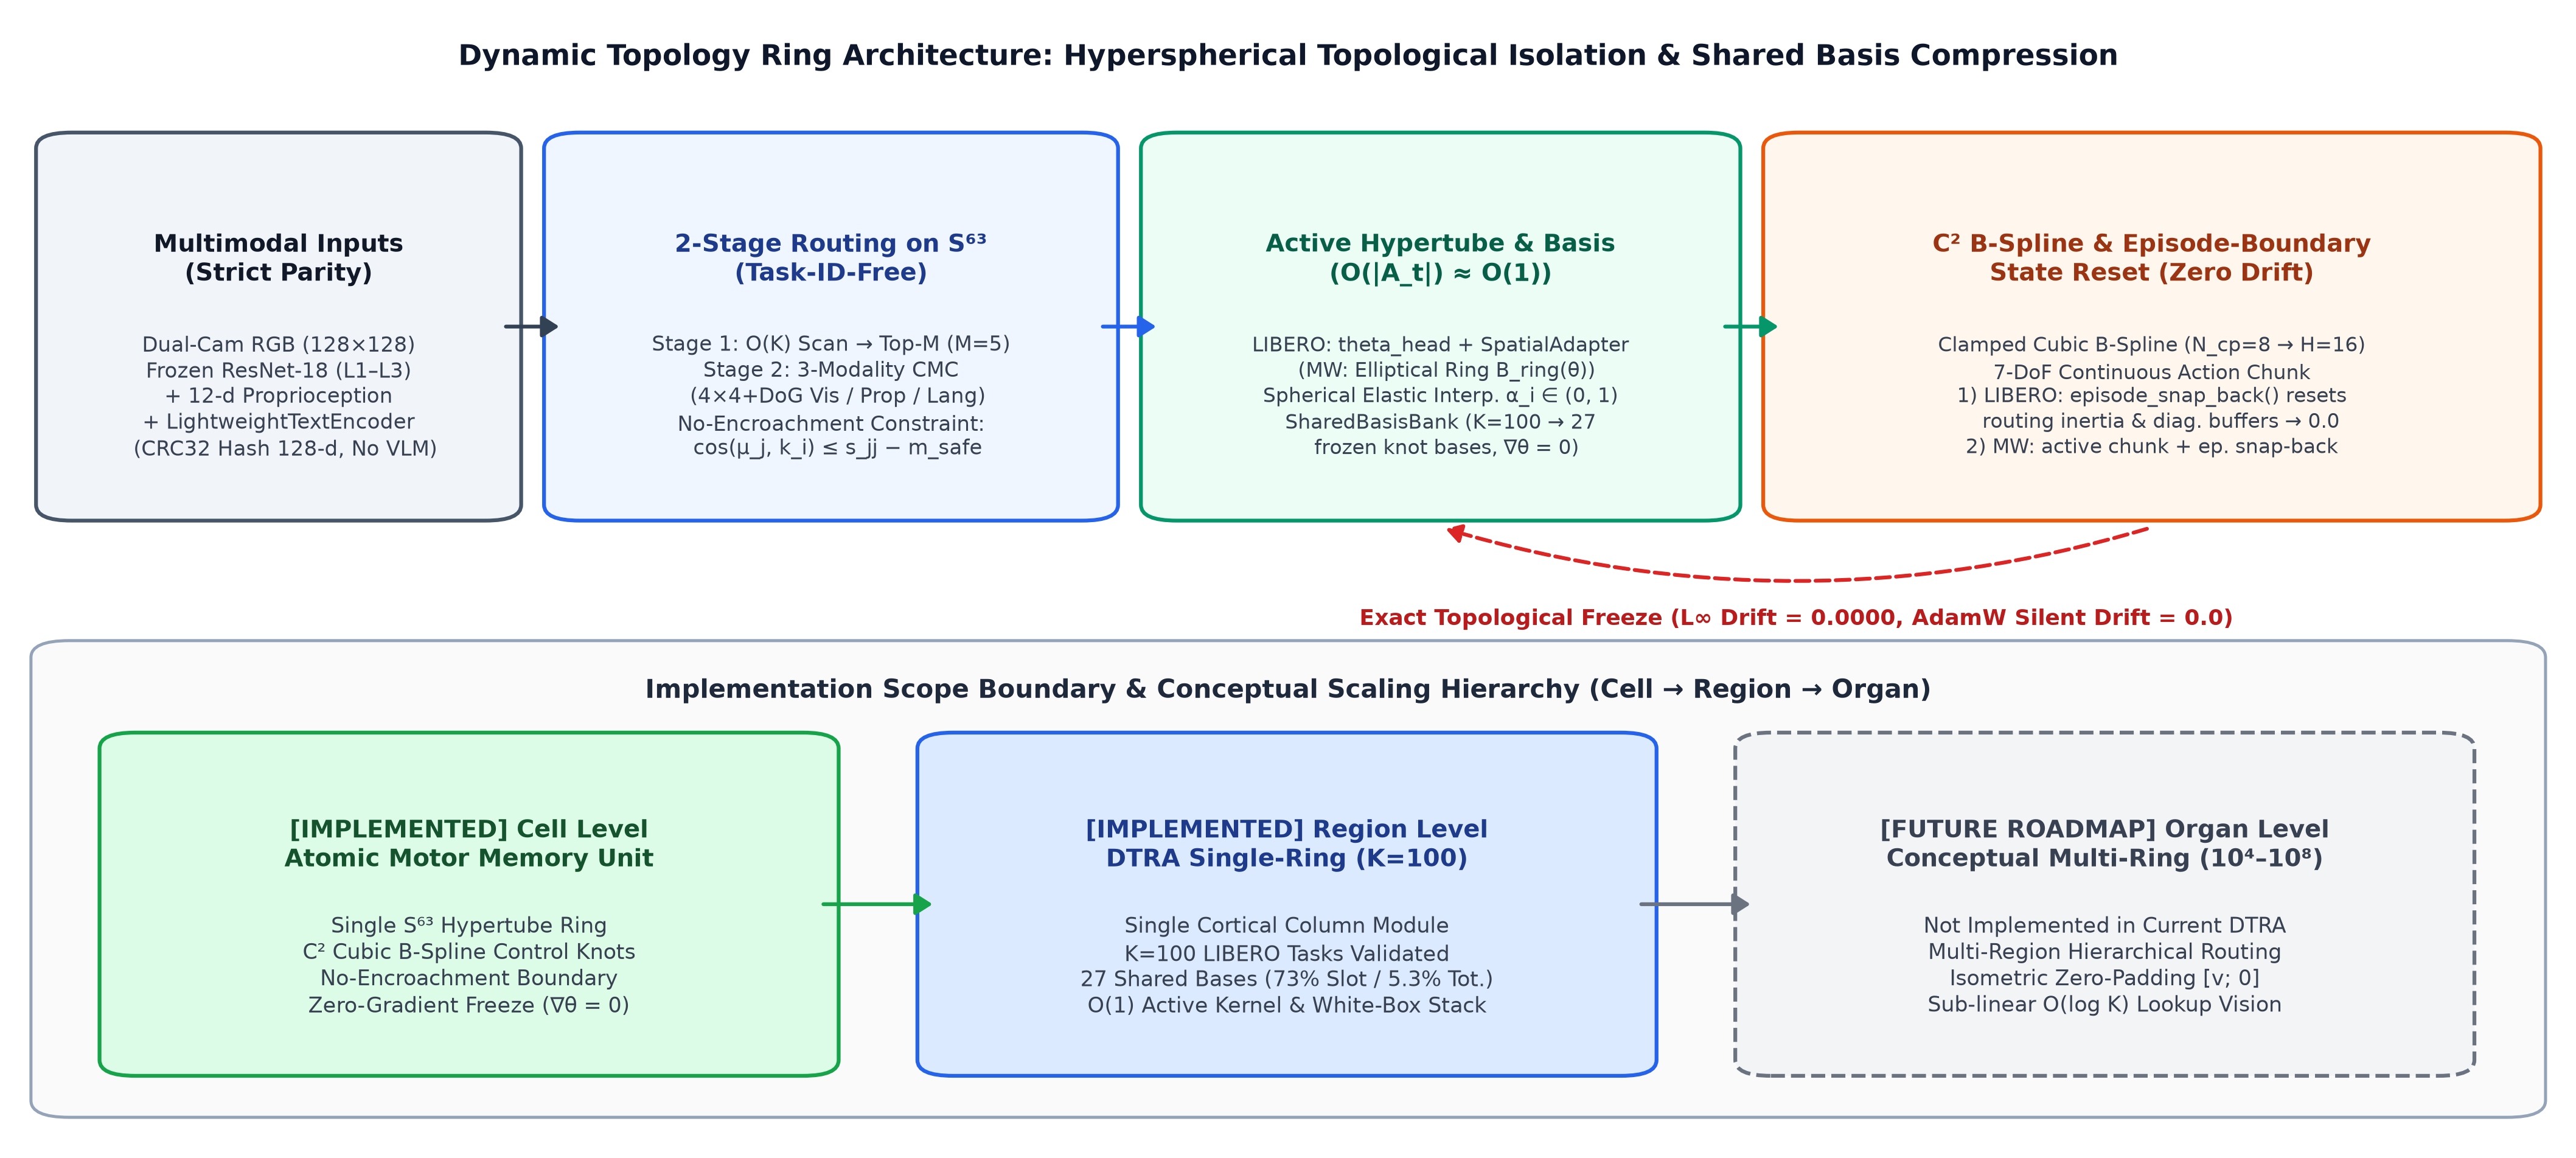
\includegraphics[width=0.78\textwidth]{../../outputs/figures/fig6_dtra_v3_architecture_schematic.png}
  \caption{\textbf{DTRA v3.0 end-to-end architecture and implementation scope boundary.} \textbf{Top:} Strict-parity multimodal perception (\texttt{Frozen ResNet-18} \texttt{L1}--\texttt{L3} + proprioception + \texttt{LightweightTextEncoder}), two-stage Top-$M$ 3-modality common-mode cancellation with No-Encroachment keys on $\mathbb{S}^{63}$, active hypertube + \texttt{SharedBasisBank} ($K=100 \to 27$ frozen bases), $C^2$ cubic B-Spline decoding, and episode-boundary state reset ($L_\infty$ optimizer drift $= 0.0$). Elliptical ring basis and active chunk snap-back apply to Meta-World; LIBERO-100 uses \texttt{theta\_head} and episode-boundary inertia reset with write-only diagnostic buffers (Sections~\ref{sec:node_arch} \&~\ref{sec:state_reset}). \textbf{Bottom:} Explicit scope separation between the implemented \emph{Cell} / single-ring \emph{Region} ($K=100$) modules validated in this paper and the conceptual \emph{Organ} ($10^4\text{--}10^8$ tasks) future work roadmap.}
  \label{fig:dtra_v3_arch}
\end{figure}

\textbf{Core Contributions (v3.0 Region Scope).}
DTRA~v3.0 addresses these challenges under matched frozen-encoder parity:
\begin{itemize}[leftmargin=*,itemsep=1.5pt,topsep=2pt]
  \item \textbf{No-Encroachment Margin Refinement:} Caches prior anchors $\mu_j$, self-similarity floors $s_{jj} = \cos(\mu_j, \mathbf{k}_j)$, and lightweight key-validation exemplars ($\le 96$ query vectors/task; no raw image/action replay) to prevent new keys from encroaching on prior Voronoi cells.
  \item \textbf{Two-Stage Top-$M$ 3-Modality CMC:} Retrieves Top-$M$ ($M=5$) candidates via $O(K)$ cosine scan, then conditionally strips candidate-local common modes across dedicated visual ($4\times 4+2\times 2+\text{DoG}$), proprioceptive, and language banks, lifting $K=100$ \texttt{Dup-Lang} routing from $41.76 \pm 2.56$\% to $\mathbf{99.68 \pm 0.55}$\%.
  \item \textbf{\texttt{SharedBasisBank} + Zero \texttt{AdamW} Silent Drift:} Compresses $100$ knot-decoder bases into \textbf{27 shared frozen bases (73\% basis-slot reduction; 5.33\% total parameter reduction)} while excluding frozen modules from \texttt{AdamW} (\texttt{requires\_grad=False}, $L_\infty$ silent drift $= 0.0$).
  \item \textbf{Empirical LIBERO-100 \& Meta-World Verification:} Establishes $\mathbf{87.00 \pm 1.06}$\% ($N=3$, $n=5$) and $\mathbf{85.20 \pm 0.43}\%$ across $12{,}000$ zero-retrain rollouts ($n=20$, held-out \texttt{init[5:20]}: $\mathbf{84.80 \pm 0.44}\%$) on LIBERO-100, alongside a 3-seed Meta-World causal ablation isolating Conv4 feature regularization.
\end{itemize}

% ==========================================================================
\section{Related Work}
\label{sec:related}
% ==========================================================================

\subsection{Continual Learning and Parameter Isolation}
Continual learning algorithms negotiate the stability--plasticity dilemma~\cite{mccloskey1989catastrophic,french1999catastrophic,parisi2019continual}. Regularization methods such as Elastic Weight Consolidation (EWC)~\cite{kirkpatrick2017ewc}, Synaptic Intelligence (SI)~\cite{zenke2017si}, Memory Aware Synapses (MAS)~\cite{aljundi2018mas}, and Riemannian Walk~\cite{chaudhry2018rwalk} penalize quadratic drift around prior optima, yet still fail when sequential gradients overwrite sensitive low-level visuomotor pathways. Rehearsal methods such as GEM~\cite{lopezpaz2017gem}, A-GEM~\cite{chaudhry2019agem}, Experience Replay (CLEAR)~\cite{rolnick2019clear}, and Dark Experience Replay (DER++)~\cite{buzzega2020der} buffer historical demonstrations, sacrificing pure replay-free autonomy and struggling when buffer capacity saturates at $K=100$. Even in continual LLM fine-tuning, recent studies show that while on-policy replay reduces short-horizon drift~\cite{chen2026opr}, composing generative replay, self-distillation, weight regularization, and merged LoRA across $100$ sequential tasks still leaves substantial long-horizon forgetting~\cite{zhang2026composecl}, motivating strict parameter isolation at $K=100$.

Parameter-isolation architectures---including Progressive Neural Networks~\cite{rusu2016pnn}, PackNet~\cite{mallya2018packnet}, and Hard Attention to the Task~\cite{serra2018hat}---prevent gradient interference structurally, yet either require ground-truth test-time Task-IDs or scale linearly in active forward compute. In lifelong robot manipulation specifically, \textbf{BUDS}~\cite{zhu2022buds} and \textbf{LOTUS}~\cite{wan2024lotus} discover hierarchical reusable skills for continual imitation learning (including real-robot validation in LOTUS), while \textbf{TAIL}~\cite{liu2024tail} isolates task-specific PEFT adapters atop large pretrained models with low per-task memory overhead. Prompt-pool approaches such as L2P~\cite{wang2022l2p}, DualPrompt~\cite{wang2022dualprompt}, and CODA-Prompt~\cite{smith2023coda} route frozen vision backbones without Task-IDs, and are evaluated alongside DER++ and O-LoRA under matched frozen-encoder parity in Section~\ref{sec:experiments}. Table~\ref{tab:paradigm_compare} contrasts these paradigms structurally against DTRA~v3.0.


\begin{table}[ht!]
  \centering
  \caption{Structural comparison of continual visuomotor control paradigms. DTRA~v3.0 combines Task-ID-free inference, zero raw-demonstration replay (retaining lightweight 96-vector key-validation exemplars per task during registration), exact parameter freezing ($\nabla_\theta = 0$), constant $O(1)$ active decoding core, and shared knot bases within a white-box routing stack.}
  \label{tab:paradigm_compare}
  \fontsize{7.7pt}{9.5pt}\selectfont
  \setlength{\tabcolsep}{1.9pt}
  \begin{tabular}{lccccccc}
    \toprule
    \textbf{Paradigm / Method} & \textbf{Task-Free} & \textbf{No Raw Rep.} & \textbf{$\nabla_\theta=0$} & \textbf{Active} & \textbf{Scaling} & \textbf{Dup-Lang} & \textbf{No VLM} \\
    \midrule
    Naive Fine-Tuning & \checkmark & \checkmark & $\times$ & $O(1)$ & Monolith & $\times$ & \checkmark \\
    EWC / RWalk~\cite{kirkpatrick2017ewc,chaudhry2018rwalk} & \checkmark & \checkmark & $\times$ & $O(1)$ & Monolith+Pen. & $\times$ & \checkmark \\
    GEM / ER / DER++~\cite{lopezpaz2017gem,rolnick2019clear,buzzega2020der} & \checkmark & $\times$ & $\times$ & $O(1)$+Buf & Monolith & $\times$ & \checkmark \\
    PNN / PackNet~\cite{rusu2016pnn,mallya2018packnet} & $\times$ & \checkmark & Masked & $O(K)$ & Linear / Mask & N/A & \checkmark \\
    BUDS / LOTUS / TAIL~\cite{zhu2022buds,wan2024lotus,liu2024tail} & Partial & Partial & Adapter & Skill/PEFT & Sub-lin./PEFT & Partial & Mixed \\
    L2P / CODA-Prompt~\cite{wang2022l2p,smith2023coda} & \checkmark & \checkmark & Backb. & Pool & Prompts & Partial & ViT/CNN \\
    O-LoRA / Seq- / KeepLoRA~\cite{wang2023olora,parsa2026seqlora,luo2026keeplora} & Depends & Mostly & Adapter & $O(r)$ & LoRA & $\times$ & VLM/MLP \\
    OrthoSkillVLA / SAMBAR~\cite{wang2026orthoskill,shrivastava2026sambar} & Depends & \checkmark & Subsp. & VLA & Subsp./Anch. & $\times$ & VLA \\
    $\text{R}^2$-WAM~\cite{fang2026r2wam} & \checkmark & Gen.Rep. & $\times$ & WAM & Video WAM & $\times$ & WAM+VLM \\
    ABK-VLA v1.1.3~\cite{son2026abkvla} & \checkmark & \checkmark & \checkmark & $O(K)$ & Linear $O(K)$ & $\times$ (DoG) & \checkmark \\
    \textbf{DTRA v3.0 (Ours)} & \textbf{\checkmark} & \textbf{\checkmark (Key Ex.)} & \textbf{\checkmark ($\bm{0}$)} & $\bm{O(1)}$ & \textbf{27b / $\bm{O(K)}$ ad.} & \textbf{\checkmark (CMC)} & \textbf{\checkmark} \\
    \bottomrule
  \end{tabular}
\end{table}


\subsection{Visuomotor Action Chunking and Continual PEFT Approaches}
Building on end-to-end deep visuomotor policies and spatial feature autoencoders~\cite{levine2016end,finn2016deep}, modern action chunking policies including ACT~\cite{zhao2023act}, Diffusion Policy~\cite{chi2023diffusion}, Octo~\cite{octo2024}, OpenVLA~\cite{kim2024openvla}, $\pi_0$~\cite{black2024pi0}, and 3D view transformers~\cite{shridhar2022peract,goyal2023rvt} stabilize closed-loop control by predicting temporally extended trajectories, whereas classical movement primitives (DMPs~\cite{ijspeert2013dmp}, ProMP~\cite{paraschos2013promp}) and spline frameworks~\cite{piegl1997nurbs,deboor1978splines} represent motions analytically. Extending ABK-VLA~\cite{son2026abkvla}, DTRA compresses chunks into smooth $C^2$-continuous cubic B-Spline knots.

In continual parameter-efficient fine-tuning (PEFT)~\cite{hu2022lora}, gradient projection memory~\cite{saha2021gpm} and orthogonal LoRA variants such as O-LoRA~\cite{wang2023olora}, InfLoRA~\cite{liang2024inflora}, residual-gradient adaptation in \textbf{KeepLoRA}~\cite{luo2026keeplora} (continual VLM and visual classification), and diffusion-domain bilevel orthogonal LoRA in \textbf{SeqLoRA}~\cite{parsa2026seqlora} (multi-concept text-to-image generation) constrain adapter updates inside shared matrices. Extending replay-free continual adaptation into robotic foundation models, \textbf{OrthoSkillVLA}~\cite{wang2026orthoskill} applies gradient-informed orthogonal subspace constraints and MoE heads to pretrained VLAs across skill-incremental LIBERO subsets; \textbf{SAMBAR}~\cite{shrivastava2026sambar} formulates replay-free VLA adaptation as constrained optimization via the method of multipliers with selective parameter anchoring; and \textbf{$\text{R}^2$-WAM}~\cite{fang2026r2wam} performs data-free continual learning in video-based World Action Models via rectified generative rollout replay with an agentic VLM evaluator. Because these methods rely on large pretrained VLA or video-generation WAM backbones evaluated under suite- or skill-incremental curricula rather than a single VLM-free $100$-task sequential stream, we discuss them structurally without direct numerical ranking, while directly benchmarking published continual learning baselines (EWC, ER, DER++, L2P, and O-LoRA) under strict matched-encoder parity.

% ==========================================================================
\section{Mathematical Preliminaries}
\label{sec:prelim}
% ==========================================================================

\subsection{Strict-Parity Multimodal Hyperspherical Embedding (\texorpdfstring{$\mathbb{S}^{63}$}{S63})}
At each control step $t$, all compared parity arms share an identical feature extractor $\mathcal{E}(\cdot)$ combining:
\begin{enumerate}[leftmargin=*,itemsep=1.5pt]
  \item \textbf{Dual-Camera Visual Encoding:} On LIBERO-100, agent-view and wrist-camera RGB frames pass through a frozen ImageNet-pretrained \texttt{ResNet-18}~\cite{he2016resnet} truncated after \texttt{layer3} (\texttt{L1}--\texttt{L3}, $256\times 8\times 8$ maps), plus 12-d proprioceptive states $\mathbf{q}_t$. Stage-1 key extraction uses \texttt{GAP}+$2\times 2$ pooled features from both cameras ($2{,}560$-d), whereas Stage-2 CMC reranking extracts centered $4\times 4$+$2\times 2$+$3\times 3$ Difference-of-Gaussians (DoG) features from agent-view plus centered $2\times 2$ wrist features ($6{,}400$-d). On Meta-World, a lightweight \texttt{Conv4} + 4-d proprioception encoder is trained on Task~0 and frozen for Tasks~1--7 alongside a fixed DoG visual key extractor.
  \item \textbf{Deterministic Text Instruction Hashing:} Instructions are encoded deterministically by \texttt{Lightweight}\allowbreak\texttt{TextEncoder} without learned LLM weights into unit vector $\ell_{\text{task}}$ (CRC32 hashing of word unigrams, bigrams, trigrams, and character 2-, 3-, and 4-grams into $128$-d on LIBERO-100; SHA-256 word unigrams + character 3-grams with fixed $512 \to 64$ QR projection on Meta-World).
\end{enumerate}
On Meta-World, 64-d QR-projected visual and language halves are concatenated on $\mathbb{S}^{127}$ and mapped via a linear layer (\texttt{proj\_topo}, learned on Task~0 and frozen thereafter) onto $\mathbb{S}^{63}$. On LIBERO-100, inspired by hyperdimensional random projections~\cite{kanerva2009hdc}, \texttt{Multimodal}\allowbreak\texttt{Magnetic}\allowbreak\texttt{KeyExtractor} maps visual, proprioceptive, and language features via three fixed Gaussian projection matrices into $\mathbb{R}^{64}$ and normalizes their weighted combination onto the unit hypersphere:
\begin{equation}
  \mathbf{c}_t = \mathrm{norm}\bigl(0.25\,\mathbf{k}_v(\mathbf{v}_t) + 0.10\,\mathbf{k}_p(\mathbf{q}_t) + 0.65\,\mathbf{k}_\ell(\ell_{\text{task}})\bigr) \in \mathbb{S}^{63}, \qquad \|\mathbf{c}_t\|_2 = 1.
\end{equation}

\subsection{Clamped \texorpdfstring{$C^2$}{C2} Cubic B-Spline Action Chunking (\texorpdfstring{$N_{\text{cp}} \in \{6,8\} \to H = 16$}{Ncp in 6,8 -> H=16})}
Rather than predicting $H \times d_a$ raw joint/delta actions directly at every control tick, DTRA encodes each chunk $\mathbf{A}_t \in \mathbb{R}^{16 \times d_a}$ in a clamped cubic B-Spline control-point subspace $\mathbf{P}_t \in \mathbb{R}^{N_{\text{cp}} \times d_a}$ via a fixed, frozen synthesis matrix $\mathbf{B}_{\text{spline}} \in \mathbb{R}^{16 \times N_{\text{cp}}}$ ($N_{\text{cp}}=8$ on 7-DoF LIBERO-100; $N_{\text{cp}}=6$ on 2D/Meta-World):
\begin{equation}
  \mathbf{A}_t = \mathbf{B}_{\text{spline}} \mathbf{P}_t, \qquad \sum_{n=0}^{N_{\text{cp}}-1} (\mathbf{B}_{\text{spline}})_{h,n} = 1 \;\; \forall h \in \{0,\dots,15\},
\end{equation}
executing the first \texttt{exec\_steps=8} steps in closed-loop receding horizon before re-querying. This parameterization yields within-chunk $C^2$ continuity and convex-hull perturbation bounds (Proposition~\ref{prop:bspline}, Appendix~\ref{app:proofs}).

\subsection{Spherical Voronoi Partitioning \& High-Density Collision Failure}
Let $\{\mathbf{k}_j\}_{j=1}^{K} \subset \mathbb{S}^{63}$ denote consolidated routing keys. Standard 1-stage cosine routing assigns $\mathbf{c}_t$ to Voronoi cell $\mathcal{V}_j = \{\mathbf{c} \in \mathbb{S}^{63} : \langle \mathbf{c}, \mathbf{k}_j \rangle \ge \langle \mathbf{c}, \mathbf{k}_i \rangle \;\forall i\}$. Unlike balanced multi-class training where prototypes naturally converge toward equiangular separation~\cite{papyan2020neural}, dense sequential $K=100$ streams contain $30$ \texttt{Dup-Lang} tasks sharing identical instructions across distinct scenes (weighted $0.65$ in $\mathbf{c}_t$). Naive contrastive repulsion during task-$k$ training can push $\langle \mu_j, \mathbf{k}_k \rangle$ past task $j$'s own anchored similarity $s_{jj} = \langle \mu_j, \mathbf{k}_j \rangle$, causing test queries $\mu_j$ to flip into cell $\mathcal{V}_k$ despite identical weight freezing on $\mathbf{k}_j$.

% ==========================================================================
\section{Method: DTRA v3.0 Architecture}
\label{sec:method}
% ==========================================================================

Algorithm~\ref{alg:dtra_v3} summarizes the complete LIBERO-100 registration and closed-loop inference pipeline, and Figure~\ref{fig:manifold_snapback} illustrates hyperspherical isolation and elastic compliance on Meta-World.

\subsection{Hypertube Node Architecture (Meta-World v2.1 vs.\ LIBERO-100 v3.0)}
\label{sec:node_arch}
Each consolidated task $i \in \{1,\dots,K\}$ owns an isolated node on $\mathbb{S}^{63}$ with unit routing anchor $\mathbf{k}_i \in \mathbb{S}^{63}$ and bounded elastic compliance $\alpha_i = \sigma(\omega_i) \in (0,1)$:
\begin{itemize}[leftmargin=*,itemsep=1.5pt]
  \item \textbf{Meta-World (\texttt{HypertubeNode}):} Allocates a Coarse/Fine tube pair per task ($8$ task pairs $= 16$ tubes) storing explicit first-order Fourier ring coefficients $\mathbf{r}_i(\theta) = \mathbf{a}_{i,0} + \mathbf{a}_{i,1}\cos\theta + \mathbf{a}_{i,2}\sin\theta$ with a closed-form first-order \texttt{atan2} phase approximation and frozen activation gate $\tau_i$.
  \item \textbf{LIBERO-100 (\texttt{LIBEROHypertubeNode}):} To scale to 7-DoF dual-camera manipulation, each node pairs a per-task \texttt{SpatialContextAdapter} ($175\,$k params) with a lightweight 2-layer MLP \texttt{theta\_head} predicting normalized phase coordinates $[1, u_1, u_2]$, followed by spherical L2-normalized elastic interpolation $\mathbf{z}_{\text{eff}} = \mathrm{norm}(\mathbf{z}_{\text{base}} + \alpha_i(\mathbf{c}_t - \mathbf{z}_{\text{base}}))$ (with $\alpha_i=0$ in \texttt{DTRA Rigid}).
\end{itemize}

\subsection{No-Encroachment Margin Refinement (With Lightweight Key Exemplars)}
When registering task $k$ after freezing prior tasks $\{1,\dots,k-1\}$, DTRA~v3.0 enforces angular margin separation~\cite{deng2019arcface} without perturbing consolidated keys by caching each prior task's query centroid $\mu_j$, verified self-similarity floor $s_{jj} = \langle \mu_j, \mathbf{k}_j \rangle$, and up to $96$ normalized multimodal query vectors (\texttt{\_val\_queries}, totaling $9{,}600$ unit vectors at $K=100$; no raw images or action demonstrations are stored). Candidate key $\mathbf{k}_k$ minimizes the one-sided hinge penalty with safety margin $m_{\text{safe}} > 0$:
\begin{equation}
  \mathcal{L}_{\text{NoEnc}}(\mathbf{k}_k) = \sum_{j < k} \max\!\Bigl(0,\; \langle \mu_j, \mathbf{k}_k \rangle - (s_{jj} - m_{\text{safe}})\Bigr)^2,
\end{equation}
while checking that validation routing accuracy over cached \texttt{\_val\_queries} does not degrade on prior tasks $j < k$ (keeping $\nabla_{\mathbf{k}_j} = 0$).

\subsection{Two-Stage Top-\texorpdfstring{$M$}{M} 3-Modality Common-Mode Cancellation (CMC)}
When tasks share identical language commands (\texttt{Dup-Lang}) across distinct scenes, raw 1-stage cosine scores suffer common-mode compression because language dominates ($0.65$ weight). DTRA~v3.0 splits LIBERO-100 retrieval into two lightweight steps:
\begin{enumerate}[leftmargin=*,itemsep=1.5pt]
  \item \textbf{Stage 1 ($O(K)$ Broad Scan):} Score all $K$ keys on $\mathbb{S}^{63}$ with temporal routing inertia ($\eta_{\text{inertia}}=0.20$) and Hebbian myelination bias ($\eta_{\text{myelin}}=0.25$, updated over each task's final three training epochs), retaining Top-$M$ ($M=5$) candidates $\mathcal{M}_t$ and scores $s_1(t, j)$.
  \item \textbf{Stage 2 (Conditional 3-Modality Differential Reranking):} Maintain separate signature banks for visual ($256$-d projection of $6{,}400$-d $4\times 4+2\times 2+\text{DoG}$ features), proprioceptive ($12$-d), and language ($128$-d) prototypes. Reranking triggers whenever $\ge 2$ candidates share exact/near-duplicate language similarity ($>0.998$ or $>0.88$ within score gap $<0.12/0.06$) or the Top-1/Top-2 margin is $<0.025$, forming candidate subset $\mathcal{C}_t \subseteq \mathcal{M}_t$. Subtracting the subset mean $\bar{\mathbf{m}}_{\text{cm}} = \frac{1}{|\mathcal{C}_t|}\sum_{j \in \mathcal{C}_t} \mathbf{m}_j$ per modality (with per-dimension z-scoring on proprioception) yields an additive residual score:
  \begin{equation}
    \tilde{\mathbf{m}}_t = \mathrm{norm}\!\bigl(\mathbf{m}_t - \bar{\mathbf{m}}_{\text{cm}}\bigr), \qquad
    i^* = \arg\max_{j \in \mathcal{C}_t} \Bigl[ s_1(t, j) + \sum_{m \in \{v,p,\ell\}} w_m \langle \tilde{\mathbf{m}}_t,\, \tilde{\mathbf{m}}_j \rangle \Bigr],
  \end{equation}
  where exact duplicate-language collisions set $(w_\ell, w_v, w_p) = (0.0, 0.25, 0.04)$ (shifting discrimination cleanly to $4\times 4+\text{DoG}$ visual and proprioceptive residuals), while near-duplicate cases use $(0.20, 0.04, 0.01)$. Note that \texttt{Frozen MLP} uses 1-stage $2\times 2$ key routing without this $4\times 4+\text{DoG}$ CMC bank (discussed in Section~\ref{sec:discussion}).
\end{enumerate}

\subsection{\texttt{SharedBasisBank} Compression \& Exact Parameter Accounting}
DTRA maintains an expandable \texttt{SharedBasisBank} $\mathcal{B} = \{\mathbf{B}_b\}_{b=1}^{B}$ of frozen B-Spline knot-decoder slots ($37{,}016$ params / $0.141\,$MB per slot; hard cap $B \le 48$). During task-$k$ registration, DTRA computes a normalized task motion signature $\mathbf{s}_k^{\text{mot}} = \mathrm{norm}([\bar{\mathbf{P}}_k, \overline{|\Delta\mathbf{P}_k|}])$ from $256$ demonstration control-point samples; if its maximum cosine similarity against stored basis signatures meets threshold $0.88$, node $k$ binds to existing basis $\mathbf{B}_{b_k}$, else a new basis is appended. Inside \texttt{LIBEROHypertubeNode}, the shared basis output blends with a per-task micro-residual ($0.55\,\mathbf{p}_{\text{basis}} + 0.45\,\mathbf{p}_{\text{micro}}$) gated onto a coarse anchor. On LIBERO-100, the bank saturates sub-linearly at $7 \to 13 \to 22 \to 24 \to \mathbf{27}$ bases across all three seeds---a \textbf{73\% reduction in basis slot count} ($3.81\,$MB vs.\ $14.12\,$MB unshared). Crucially, however, each task still instantiates an isolated \texttt{LIBEROHypertubeNode} adapter ($470\,$k params / $1.79\,$MB $\times 100 = 179.33\,$MB, $97.92\%$ of total policy memory). Thus \texttt{SharedBasisBank} yields a \textbf{5.33\% total policy-parameter reduction} ($193.45 \to 183.14\,$MB), leaving total memory $O(K)$ ($+20.75\%$ vs.\ Frozen MLP's $151.67\,$MB). Every consolidated basis and node receives \texttt{requires\_grad=False} and is excluded from downstream \texttt{AdamW} parameter groups ($L_\infty = 0.0$, Proposition~\ref{prop:zero_drift}).

\subsection{Episode-Boundary State Reset \& Diagnostic Logging}
\label{sec:state_reset}
At episode termination, \texttt{episode\_snap\_back()} resets active routing inertia (\texttt{prev\_selected}, \texttt{prev\_act\_vec}) and diagnostic deformation buffers to exact $0.0000$ (\texttt{post\_snap\_norm}) so no state leaks across episodes. On Meta-World, elastic deformation operates directly on the ring phase residual and resets after each chunk via \texttt{snap\_back()} (Figure~\ref{fig:manifold_snapback}); on LIBERO-100, \texttt{LIBEROHypertubeNode} is a 1-step Markov decoder whose \texttt{episodic\_trace} and \texttt{delta\_z\_state} buffers are write-only diagnostic tensors (logged and zeroed at chunk/episode boundaries without feeding back into \texttt{forward()}), so \texttt{chunk\_snap\_back()} does not alter LIBERO-100 control outputs.


\begin{algorithm}[ht!]
\caption{\textbf{DTRA v3.0 Training Registration \& Closed-Loop Control (LIBERO-100 Implementation)}}
\label{alg:dtra_v3}
\small
\begin{algorithmic}[1]
\Require Frozen DualCam \texttt{ResNet-18} (\texttt{L1}--\texttt{L3}) + proprioception + \texttt{LightweightTextEncoder}; frozen \texttt{SharedBasisBank} $\mathcal{B} = \{\mathbf{B}_b\}_{b=1}^{B}$ (LIBERO-100: $N_{\text{cp}}=8$ clamped cubic B-Spline knots $\to H=16$; Meta-World: $N_{\text{cp}}=6$); empty cell registry $\mathcal{C} = \emptyset$.
\Statex \textbf{Phase I: Sequential Continual Registration ($k = 1, \dots, K$, Task-ID Stored Only for Audit)}
\State Project Stage-1 visual (\texttt{GAP}+$2\times 2$), proprioceptive, and language features into normalized query $\mathbf{c}_t \in \mathbb{S}^{63}$ via fixed Gaussian projections ($0.25\mathbf{k}_v + 0.10\mathbf{k}_p + 0.65\mathbf{k}_\ell$ on LIBERO-100); compute task prototype $\mu_k$ and 3-modality Stage-2 signature prototypes $(\mathbf{v}_k^{\text{sig}}, \mathbf{p}_k^{\text{sig}}, \boldsymbol{\ell}_k^{\text{sig}})$ using $4\times 4+2\times 2+\text{DoG}$ visual features.
\State Refine routing key $\mathbf{k}_k$ against prior tasks $\{j < k\}$ subject to \textbf{No-Encroachment}: penalize $\langle \mu_j, \mathbf{k}_k \rangle > s_{jj} - m_{\text{safe}}$ and verify accuracy on cached lightweight key-validation exemplars ($\le 96$ normalized query vectors/task, \texttt{\_val\_queries}; no raw image/action replay).
\State Fit $C^2$ clamped cubic B-Spline knots ($\mathbf{P}_k \in \mathbb{R}^{8\times 7}$ on LIBERO-100; $\mathbb{R}^{6\times 4}$ on Meta-World) and compute normalized motion signature $\mathbf{s}_k^{\text{mot}} = \mathrm{norm}([\bar{\mathbf{P}}_k, \overline{|\Delta\mathbf{P}_k|}])$. If max cosine similarity to stored basis signatures is below $0.88$ (and $B < 48$), append new frozen basis $\mathbf{B}_{B+1}$; else bind to existing $\mathbf{B}_{b_k}$ and train per-task node adapter \texttt{LIBEROHypertubeNode} (spatial context + phase/residual heads) with \texttt{AdamW} (\texttt{weight\_decay=1e-4}, frozen params excluded).
\State Freeze all consolidated node and basis parameters permanently (\texttt{requires\_grad=False}, $\nabla_\theta = 0$, $L_\infty$ silent drift $= 0.0$).
\Statex \textbf{Phase II: No-Raw-Replay, Task-ID-Free Closed-Loop Evaluation (At Control Tick $t$)}
\State \textbf{Stage 1 ($O(K)$ Broad Scan):} Score all $K$ keys on $\mathbb{S}^{63}$ with temporal inertia ($\eta_{\text{inertia}}=0.20$) and Hebbian myelination bias ($\eta_{\text{myelin}}=0.25$), and retrieve Top-$M$ ($M=5$) candidates $\mathcal{M}_t$.
\State \textbf{Stage 2 (Conditional 3-Modality Common-Mode Cancellation):} When candidate language similarities collide or Top-1/Top-2 margin $< 0.025$, form subset $\mathcal{C}_t \subseteq \mathcal{M}_t$, subtract candidate-local means across visual ($256$-d), z-scored proprioceptive ($12$-d), and language ($128$-d) banks, and add weighted CMC residuals to Stage-1 scores to select $i^* = \arg\max_{j \in \mathcal{C}_t} s_{\text{comb}}(t, j)$.
\State Decode selected node $i^*$ and shared basis $\mathbf{B}_{b_{i^*}}$ via phase head (\texttt{theta\_head} on LIBERO-100; elliptical \texttt{atan2} on Meta-World) and bounded spherical interpolation $\alpha_{i^*}$ into $H=16$ chunk $\mathbf{A}_t = \mathbf{B}_{\text{spline}}\mathbf{P}_{\text{eff}}$; execute \texttt{exec\_steps=8} steps.
\State At episode termination, call \texttt{episode\_snap\_back()} to reset routing inertia (\texttt{prev\_selected}, \texttt{prev\_act\_vec}) and diagnostic buffers to exact $0.0000$.
\end{algorithmic}
\end{algorithm}


\begin{figure}[ht!]
  \centering
  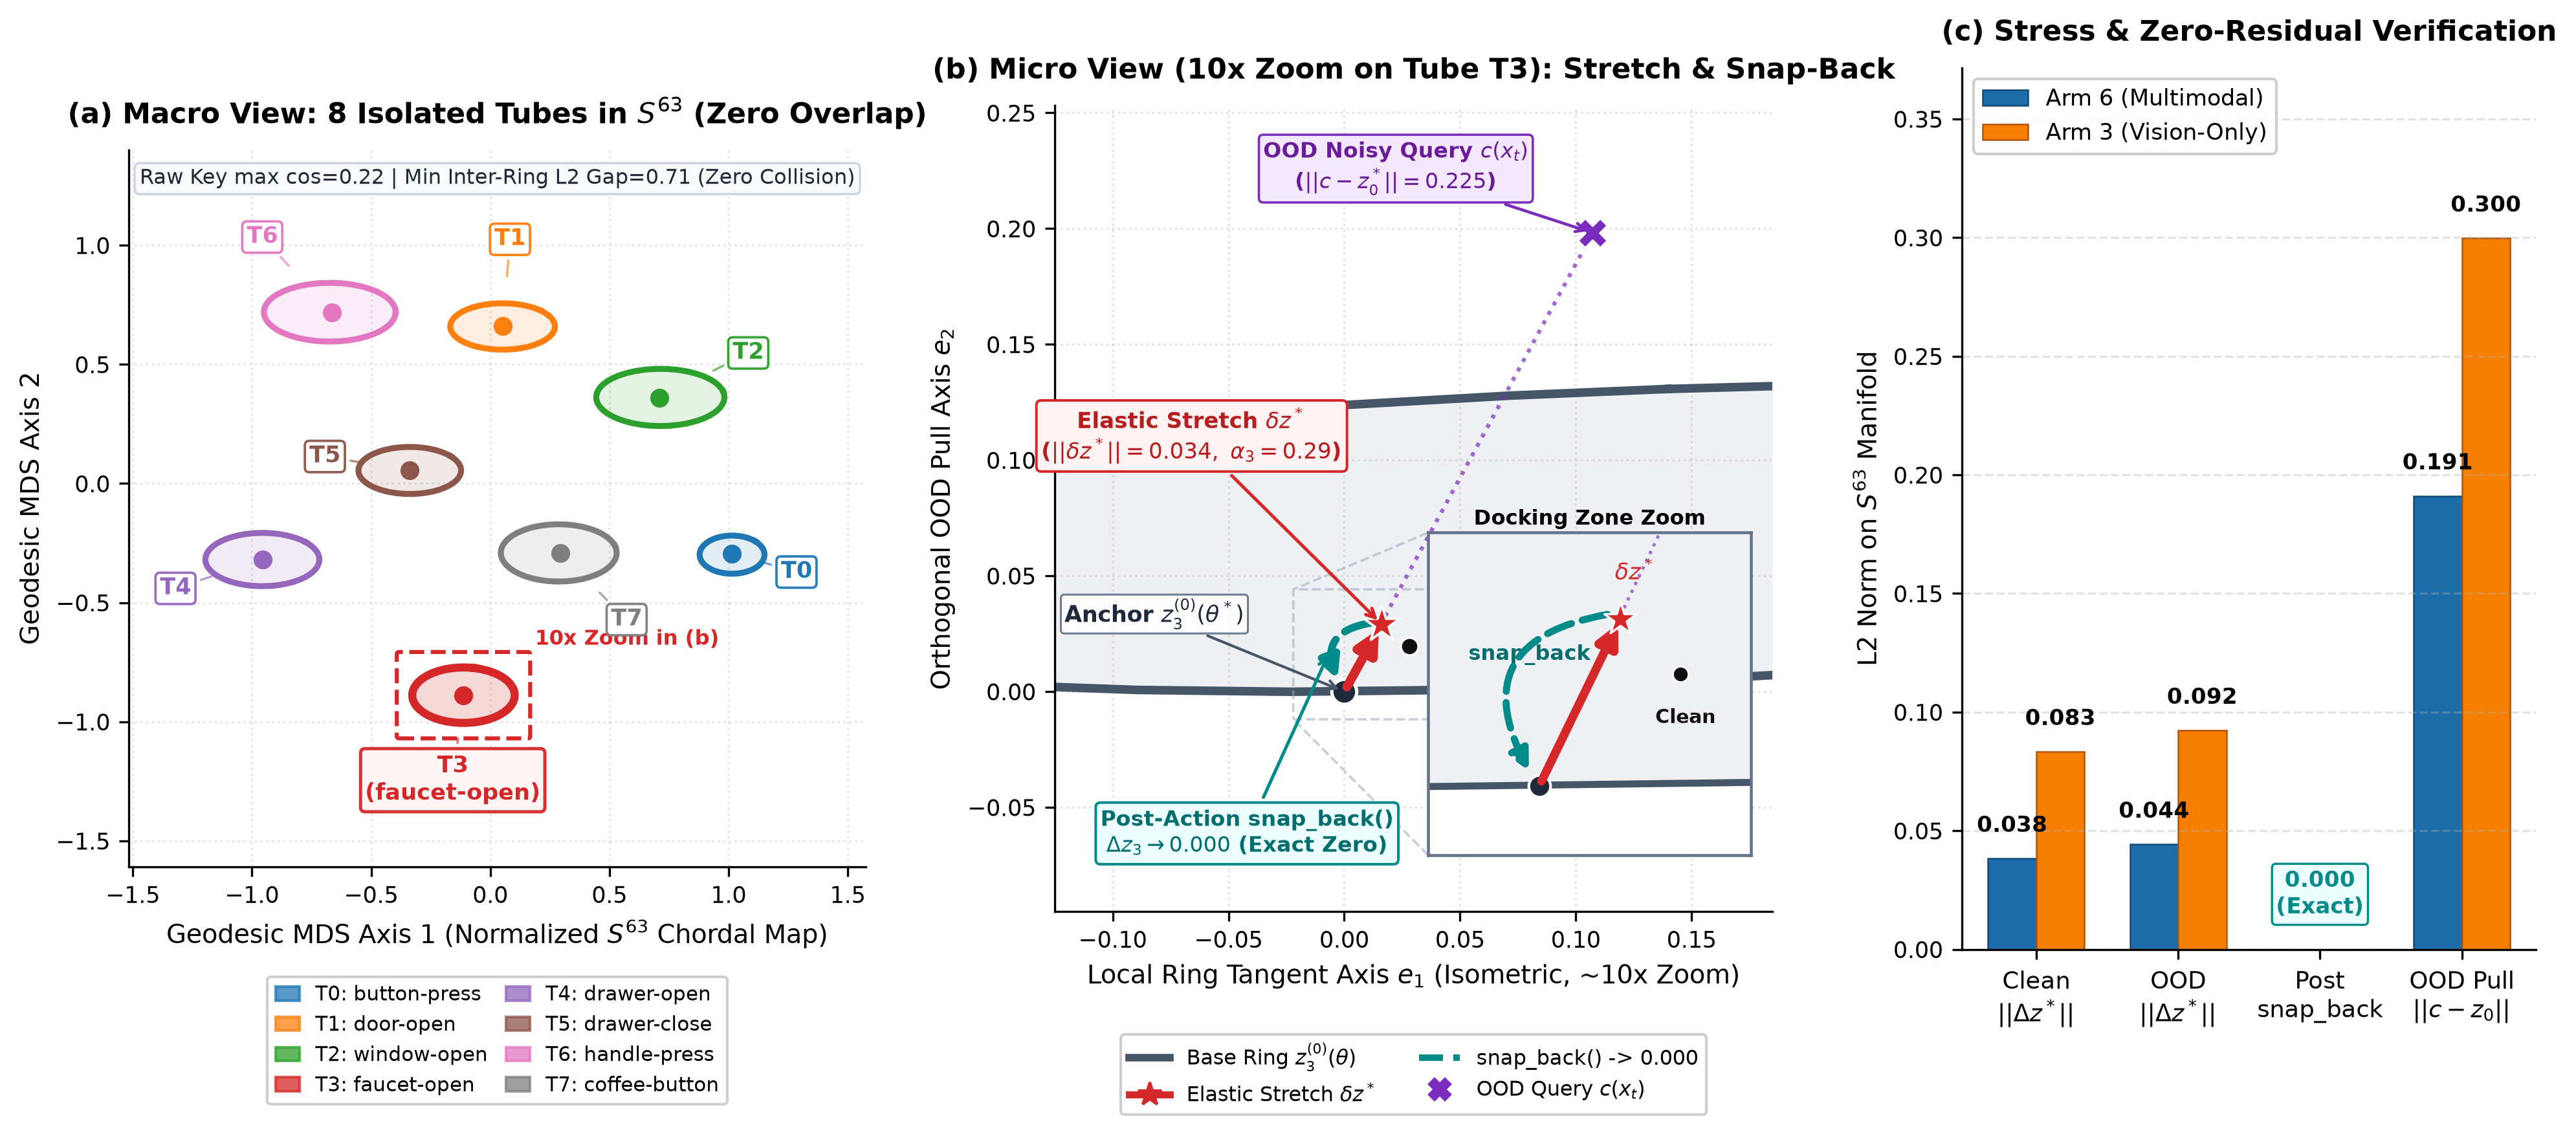
\includegraphics[width=0.80\textwidth]{../../outputs/figures/fig2_manifold_elastic_snapback.png}
  \caption{\textbf{3D Meta-World topological isolation and bounded elastic \texttt{snap\_back()} on $\mathbb{S}^{63}$ (Seed~42).} Distinct Sawyer skills ($T_0\text{--}T_7$) occupy separated elliptical hypertube rings; OOD perturbations flex active state along compliant radius $\alpha_i$ before per-chunk \texttt{snap\_back()} restores exact $0.0000$ residual drift. Panel~(c) reports Fine-tube deformation norms ($0.038$ clean / $0.044$ OOD; combined Coarse+Fine means in Appendix~Table~\ref{tab:mw_snapback}).}
  \label{fig:manifold_snapback}
\end{figure}

% ==========================================================================
\section{Experiments \& Continual Scaling Analysis}
\label{sec:experiments}
% ==========================================================================

\subsection{Strict-Parity Experimental Protocol \& Step-1 Invariants}
We evaluate all baselines and DTRA variants under strict encoder parity ($\mathcal{E}$ identical across arms, no external VLMs, full hyperparameter schedule in Appendix~Table~\ref{tab:hyperparams}; \texttt{--stream-tasks} single-task staging keeps DTRA, Frozen MLP, and O-LoRA peak VRAM $\le 2.8\,$GB on RTX~3090, while replay and prompt-pool arms require up to $6.0\,$GB, Appendix~Table~\ref{tab:libero_resources}). Prior to multi-benchmark runs, six Step-1 dynamical tests (\texttt{sim\_dtra\_}\allowbreak\texttt{tube\_dynamics.py}) and five v3.0 module tests (\texttt{test\_dtra\_}\allowbreak\texttt{v3\_modules.py}) confirm zero NaN gradients, $0.0000$ post-snap deformation, $25.0\%$ sparse active ratio ($75.0\%$ pruned), $+0.1648$ compatible recall, No-Encroachment margin retention, and exact $0.0$ \texttt{AdamW} silent drift on frozen bases.

\begin{figure}[ht!]
  \centering
  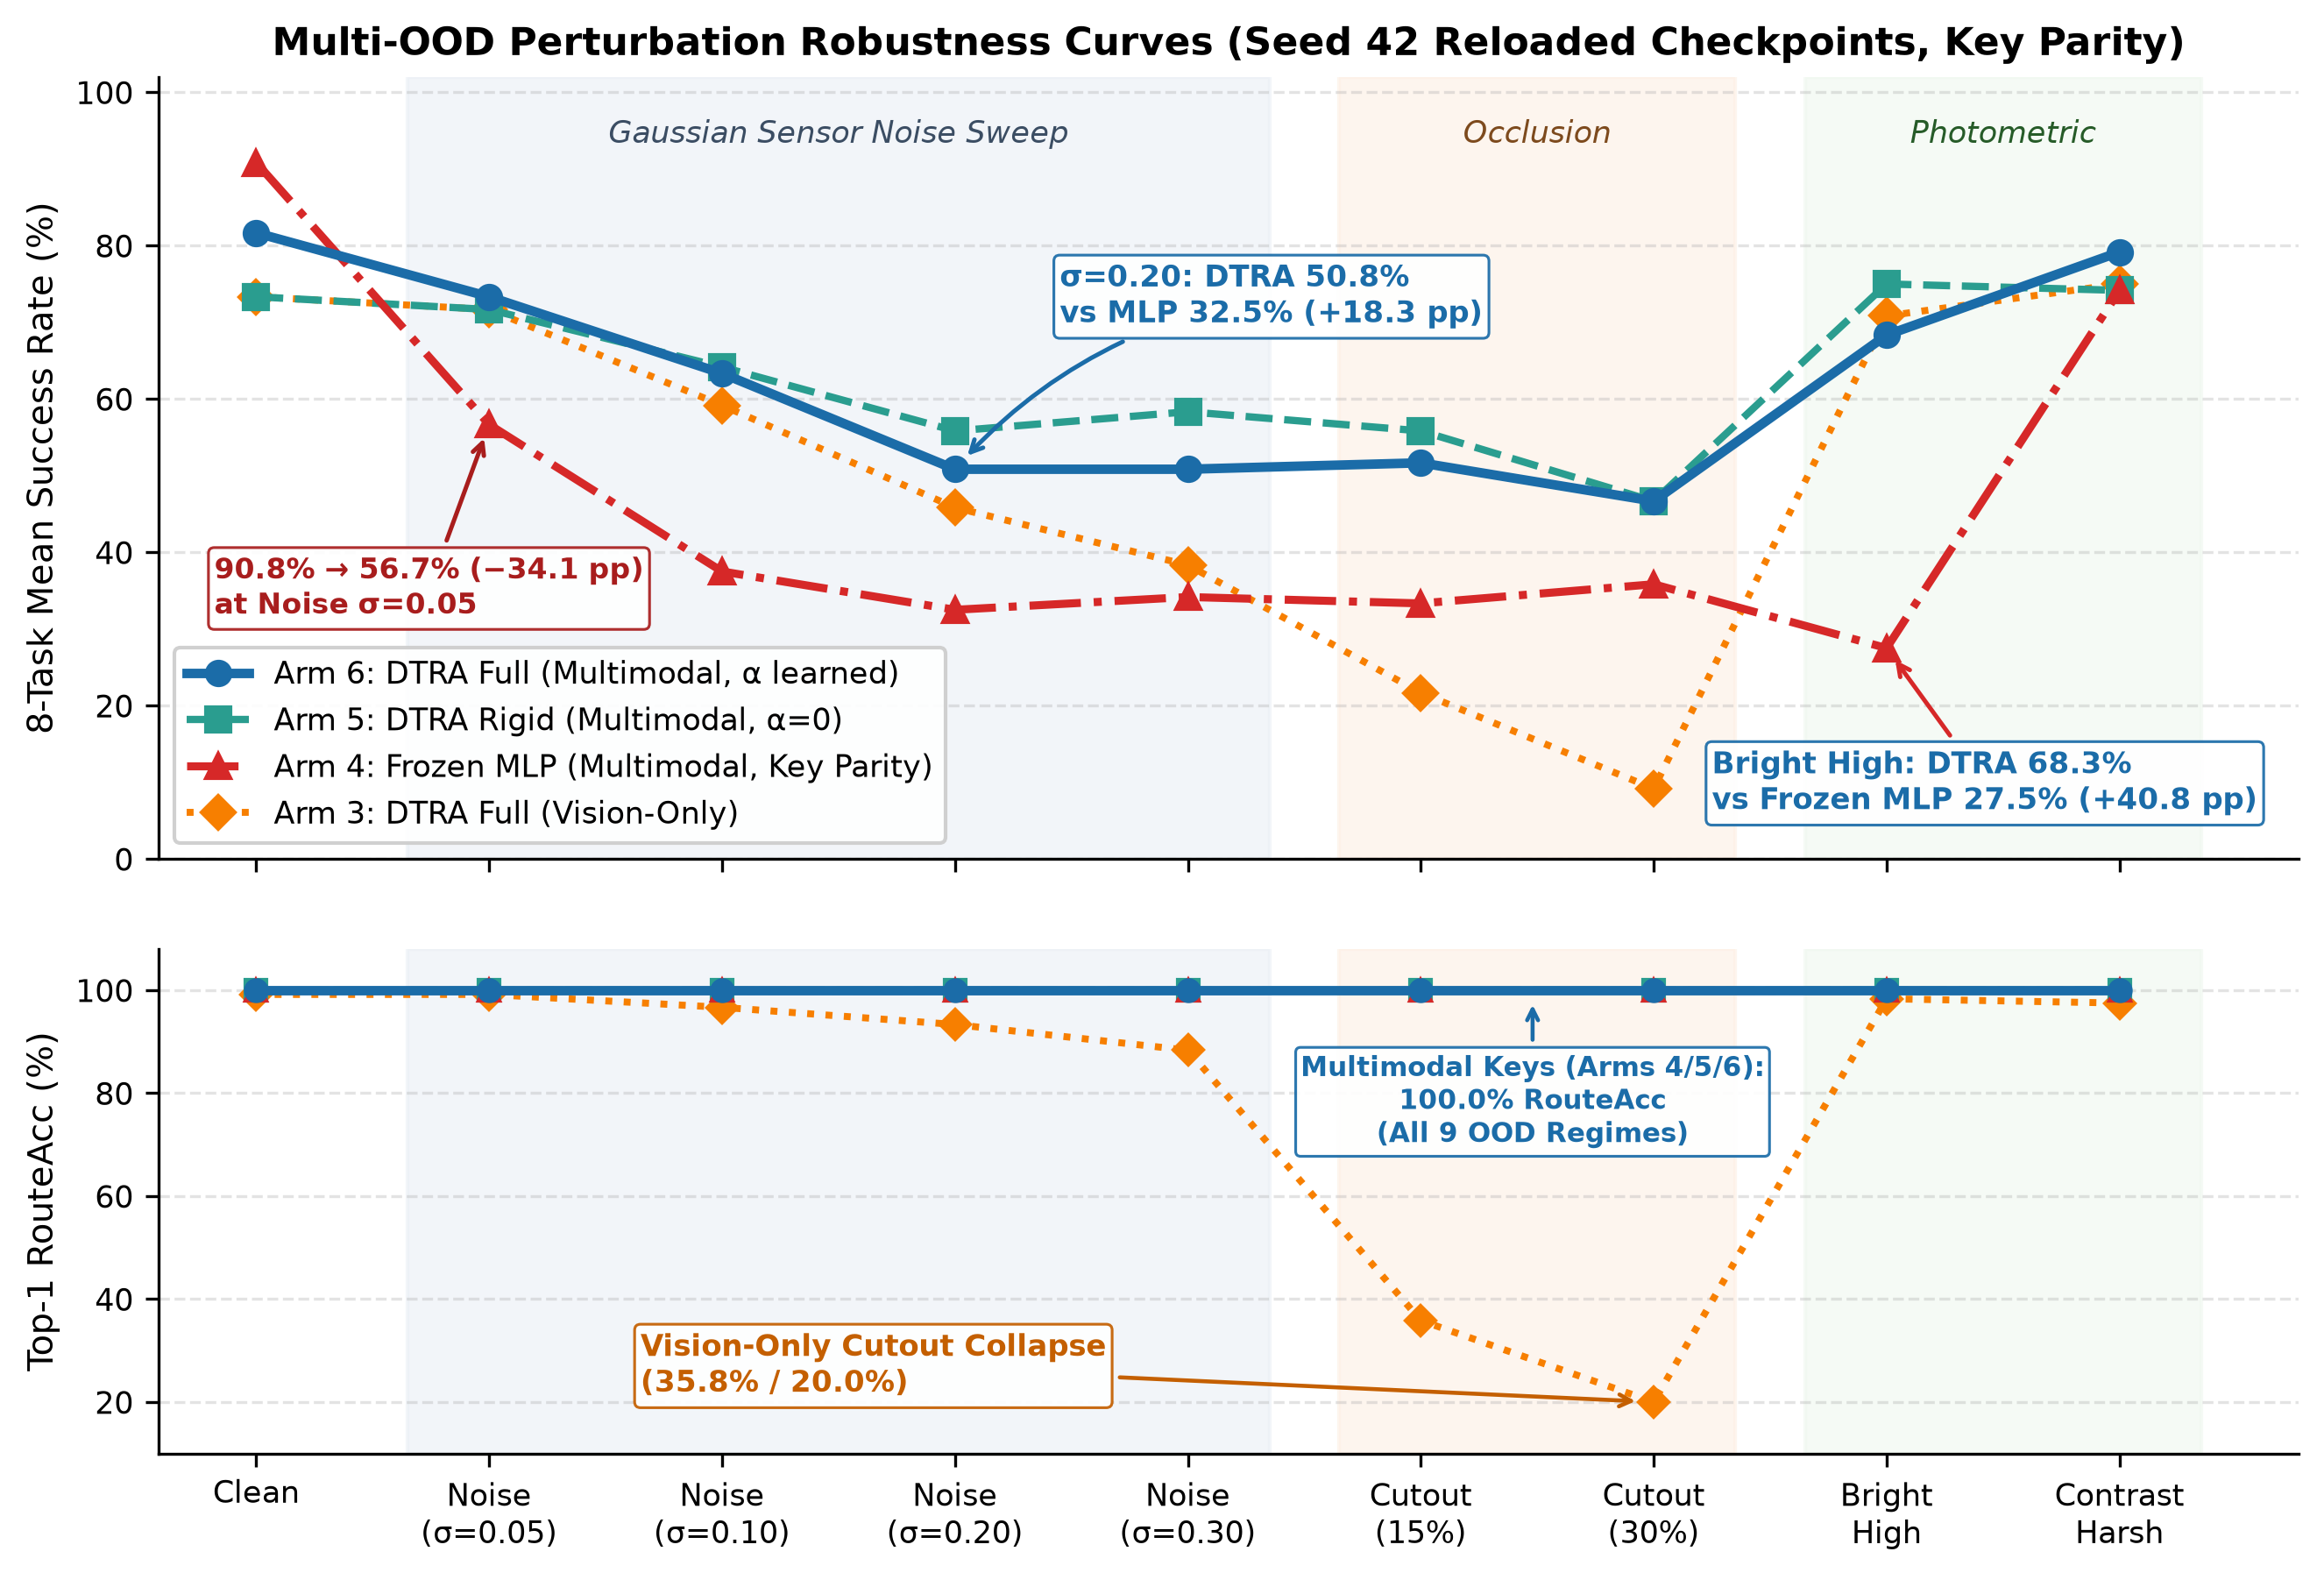
\includegraphics[width=0.78\textwidth]{../../outputs/figures/fig1_ood_perturbation_curves.png}
  \caption{\textbf{3D Meta-World 9-regime zero-shot OOD stress curves (Reloaded Seed~42 checkpoints).} Plotted curves compare DTRA Full (MM, $50.8\%$ at $\sigma=0.20$), DTRA Rigid ($55.8\%$), Frozen MLP ($32.5\%$), and DTRA Vision ($45.8\%$) across Gaussian noise ($\sigma=0.05\text{--}0.30$), $15\%/30\%$ cutout occlusion, brightness, and harsh contrast; across all 3 seeds (\texttt{ddof=1}, Table~\ref{tab:mw_3seed}), DTRA Full retains $100.0\%$ multimodal routing and $51.4 \pm 5.4\%$ severe OOD SR vs.\ $23.6 \pm 4.8\%$ for Frozen MLP.}
  \label{fig:mw_ood}
\end{figure}


\begin{table}[ht!]
  \centering
  \caption{3D Meta-World 8-Task Continual Benchmark (all rate metrics in \%; 3-Seed Mean $\pm$ Sample Std \texttt{ddof=1} over Seeds~42, 100, 2026; $n_{\text{eval}}=15$ clean / $15$ severe OOD per task, $55$ epochs/task) and CPU Active Latency ($K=1 \to 8$). Bold numbers mark the best metric per column; bold method names mark proposed DTRA variants. $^\dagger$Identical architecture/latency to DTRA Full (Feat-Reg).}
  \label{tab:mw_3seed}
  \fontsize{8.0pt}{9.8pt}\selectfont
  \setlength{\tabcolsep}{2.6pt}
  \begin{tabular}{lcccccc}
    \toprule
    \textbf{Method (Parity Arms \& External CL)} & \textbf{Clean~(\%)} & \textbf{FR~(\%)$\downarrow$} & \textbf{C.\,Rte~(\%)} & \textbf{OOD~(\%)} & \textbf{O.\,Rte~(\%)} & \textbf{CPU~(ms)} \\
    \midrule
    ABK-VLA v1.1.3 (DoG Vision) & $82.8 \pm 3.2$ & $\mathbf{0.0 \pm 0.0}$ & 99.7 & $2.2 \pm 1.3$ & 34.7 & $0.27 \to 0.83$ \\
    Frozen Slot MLP (Vision) & $45.8 \pm 4.3$ & $20.0 \pm 1.0$ & 99.2 & $25.0 \pm 3.6$ & 94.4 & $0.21 \to 0.21$ \\
    DTRA Full (Vision-Only) & $75.8 \pm 6.3$ & $\mathbf{0.0 \pm 0.0}$ & 99.2 & $52.5 \pm 12.6$ & 95.0 & $1.97 \to 1.87$ \\
    Frozen Slot MLP (Multimodal) & $\mathbf{85.6 \pm 3.8}$ & $\mathbf{0.0 \pm 0.0}$ & \textbf{100.0} & $23.6 \pm 4.8$ & \textbf{100.0} & $\mathbf{0.21 \to 0.20}$ \\
    DTRA Rigid ($\alpha=0$, MM) & $77.8 \pm 4.3$ & $\mathbf{0.0 \pm 0.0}$ & \textbf{100.0} & $\mathbf{53.6 \pm 8.3}$ & \textbf{100.0} & $1.86 \to 1.87$ \\
    \textbf{DTRA Full (Feat-Reg, Ours)} & $72.2 \pm 8.3$ & $\mathbf{0.0 \pm 0.0}$ & \textbf{100.0} & $51.4 \pm 5.4$ & \textbf{100.0} & $1.87 \to 1.87$ \\
    \textbf{DTRA Full (No Feat-Reg, Ours)} & $83.1 \pm 6.3$ & $\mathbf{0.0 \pm 0.0}$ & \textbf{100.0} & $45.0 \pm 6.6$ & \textbf{100.0} & $1.87 \to 1.87$$^\dagger$ \\
    \midrule
    DER++ (5\% Buffer + Dark Distill.) & $73.3 \pm 4.4$ & $22.9 \pm 3.3$ & --- & $13.6 \pm 8.9$ & --- & --- \\
    L2P (Prompt Pool, Replay-Free) & $16.7 \pm 4.4$ & $79.4 \pm 13.3$ & --- & $17.5 \pm 8.7$ & --- & --- \\
    O-LoRA (Ortho Subspace, Replay-Free) & $7.2 \pm 1.7$ & $63.2 \pm 6.8$ & --- & $9.4 \pm 6.3$ & --- & --- \\
    \bottomrule
  \end{tabular}
\end{table}


\subsection{3D Meta-World 8-Task Continual Ablation, Causal Decomposition \& LIBERO-Goal Pilot}
Table~\ref{tab:mw_3seed}, Appendix~\ref{app:metaworld_details} (Tables~\ref{tab:mw_pertask}--\ref{tab:mw_snapback}), and Figure~\ref{fig:mw_ood} evaluate sequential 3D manipulation on Meta-World~\cite{yu2020metaworld}, showing that shared-backbone and parameter-efficient continual baselines degrade across tasks: across three seeds (Mean $\pm$ Sample Std \texttt{ddof=1}, $\sim 5.25\,$M matched capacity), \texttt{DER++}~\cite{buzzega2020der} reaches $73.3 \pm 4.4\%$ clean SR with $22.9 \pm 3.3\%$ forgetting and $13.6 \pm 8.9\%$ severe OOD SR, while \texttt{L2P}~\cite{wang2022l2p} ($16.7 \pm 4.4\%$ clean, $79.4 \pm 13.3\%$ FR) and \texttt{O-LoRA}~\cite{wang2023olora} ($7.2 \pm 1.7\%$ clean, $63.2 \pm 6.8\%$ FR) suffer severe trajectory interference as un-isolated readout updates overwrite continuous velocity fields (alongside Seed~42 \texttt{Naive FT} $98.1\%$ FR, \texttt{EWC} $100.0\%$ FR, and \texttt{ER 5\%} $20.0\%$ FR). Furthermore, a controlled three-seed causal ablation (Appendix~Table~\ref{tab:mw_supp}) resolves the clean-versus-OOD trade-off: disabling \texttt{DenoisingFineHead}'s Conv4 feature dropout ($p=0.30$) and Gaussian feature noise ($\sigma=0.05$) lifts \textbf{DTRA Full (No Feat-Reg)} clean SR by $+10.8\,$pp (unrounded $83.06 - 72.22$) from $72.2 \pm 8.3\%$ to $\mathbf{83.1 \pm 6.3}\%$ (matching Frozen MLP's $85.6 \pm 3.8\%$) while retaining $\mathbf{45.0 \pm 6.6}\%$ severe OOD SR ($+21.4\,$pp over unregularized Frozen MLP's $23.6 \pm 4.8\%$, and $+1.7\,$pp over \texttt{DTRA Rigid No Feat-Reg} at $81.7 \pm 5.1\%$ clean / $43.3 \pm 2.2\%$ OOD). Conversely, applying identical Conv4 feature regularization to Frozen MLP yields $90.8 \pm 3.6\%$ clean and $49.2 \pm 10.1\%$ OOD SR on sparse $8$-task Meta-World, confirming that both manifold-bounded residuals and feature regularization contribute to OOD resilience, whereas DTRA's decisive structural advantage emerges at $K=100$ high-density duplicate-instruction scaling. DTRA maintains \textbf{0.0\% forgetting}, \textbf{100.0\% routing} across clean, severe OOD, and reverse ordering ($T_7 \to T_0$: $74.2\%$ clean SR, $64.2\%$ OOD SR), with flat $O(1)$ CPU active execution ($1.87 \to 1.87\,$ms from $K=1 \to 8$). On the sparse 5-task \texttt{libero\_goal} pilot (Appendix~Table~\ref{tab:libero_goal_pilot}), \texttt{arm\_frozen\_mlp} memorizes all 5 separated trajectories ($100.0\%$ SR, $0.0\%$ FR), while \texttt{arm\_dtra\_elastic} reaches $92.0\%$ SR ($5.0\%$ FR, $+0.0\%$ BWT, $100.0\%$ routing) ahead of \texttt{arm\_dtra\_rigid} ($88.0\%$, $10.0\%$ FR) and \texttt{arm\_er\_5pct} ($88.0\%$, $10.0\%$ FR).

\subsection{LIBERO-100 (\texorpdfstring{$K=10 \to 100$}{K=10 -> 100}) High-Density Scaling Benchmark}
Scaling twenty-fold to $100$ sequential 7-DoF manipulation tasks (\texttt{libero\_10} + \texttt{libero\_90}, $50$ demos/task training, $n_{\text{eval}}=5$ rollouts/task across $260$ milestone + $95$ intermediate diagonal evaluations totaling $1{,}775$ rollouts per arm, plus $n_{\text{eval}}=20$ final zero-retrain verification totaling $12{,}000$ rollouts) reverses the sparse baseline advantage completely (Tables~\ref{tab:libero100_traj}, \ref{tab:libero100_final}, and~\ref{tab:libero100_neval20}, Appendix~\ref{app:libero_details}, Figure~\ref{fig:libero100_scaling}):
\begin{enumerate}[leftmargin=*,itemsep=1.5pt,topsep=2pt]
  \item \textbf{Baseline Voronoi Collapse vs.\ DTRA Routing Preservation:} Starting from $100.0\%$ routing at $K=10$, \texttt{arm\_frozen\_mlp} collapses steadily under key interference to $\mathbf{41.76 \pm 2.56}$\% \texttt{Dup-Lang} routing at $K=100$, dragging Mean SR down to $\mathbf{70.33 \pm 1.45}$\%. DTRA's No-Encroachment refinement and 3-modality Top-$M$ CMC sustain $100.0\%$ routing through $K=70$ and $\mathbf{99.90 \pm 0.16}$\% overall / $\mathbf{99.68 \pm 0.55}$\% \texttt{Dup-Lang} at $K=100$ (\textbf{$+57.93$\,pp} over Frozen MLP).
  \item \textbf{Full $N=3$ Retention (Elastic $\approx$ Rigid):} Across all three training seeds (3-seed \texttt{\_locked.json} Mean $\pm$ Sample Std across Seeds~[42, 100, 2026], \texttt{ddof=1}), \texttt{arm\_dtra\_elastic} reaches $\mathbf{87.00 \pm 1.06}$\% Mean Final SR (\textbf{$+16.67$\,pp} over Frozen MLP) and \texttt{arm\_dtra\_rigid} reaches $\mathbf{86.67 \pm 0.81}$\% ($N=3$, $2.56 \pm 1.11$\% FR). Elastic and Rigid are statistically comparable ($+0.33\,$pp, with Rigid higher on Seed~2026: $87.6\%$ vs.\ $85.8\%$), confirming that the main LIBERO-100 gain comes from routing stability and parameter isolation rather than elastic compliance alone.
  \item \textbf{External CL Baselines at $K=100$ (Capacity \& Adaptation Caveats) \& Basis Sharing:} Under identical frozen ResNet-18 perception (Seed~42), \texttt{DER++}~\cite{buzzega2020der} ($1.70\,$MB monolithic head, 5\% buffer + distillation) declines from $68.00\%$ ($K=10$) to $38.40\%$ at $K=100$ ($29.70\%$ FR; $12.00\%$ on earliest tasks \texttt{libero\_10}), alongside \texttt{arm\_er\_5pct} ($39.47 \pm 1.81$\%, $26.33 \pm 4.24$\% FR). Naive continuous-control adaptations of \texttt{L2P}~\cite{wang2022l2p} ($1.20\%$, $51.72\%$ FR) and \texttt{O-LoRA}~\cite{wang2023olora} ($1.00\%$, $42.63\%$ FR) collapse severely; as detailed in Section~\ref{sec:discussion}, these single-network baselines operate at $88{\times}\text{--}108{\times}$ smaller parameter capacity than DTRA ($183.14\,$MB vs.\ $1.70\text{--}2.09\,$MB) and face non-transformer adaptation constraints. Meanwhile, \texttt{SharedBasisBank} saturates at \textbf{27 frozen knot bases} ($3.81\,$MB, $73\%$ basis-slot reduction / $5.33\%$ total parameter reduction).
  \item \textbf{Zero-Retrain Extended $n_{\text{eval}}=20$ Verification ($12{,}000$ Rollouts):} Evaluating all three saved $K=100$ checkpoints across $20$ initial states/task ($6{,}000$ rollouts/arm, Table~\ref{tab:libero100_neval20}) confirms zero overfitting to \texttt{init[0:5]}: \texttt{arm\_dtra\_elastic} sustains $\mathbf{85.20 \pm 0.43}\%$ overall (descriptive pooled binomial 95\% Wilson CI $[84.3, 86.1]\%$) and $\mathbf{84.80 \pm 0.44}\%$ on $15$ unseen initial states \texttt{init[5:20]} ($[83.7, 85.8]\%$), outperforming \texttt{arm\_frozen\_mlp} ($69.12 \pm 0.90\%$ overall; $68.82 \pm 0.91\%$ held-out) by $\mathbf{+16.08}\,$\textbf{pp} overall and $\mathbf{+52.72}\,$\textbf{pp} on \texttt{Dup-Lang} ($89.06\%$ vs.\ $36.33\%$; $99.94\%$ vs.\ $41.80\%$ routing), while matching on \texttt{Unique-Lang} ($83.55\%$ vs.\ $83.17\%$, $+0.38\,$pp).
\end{enumerate}

\begin{figure}[ht!]
  \centering
  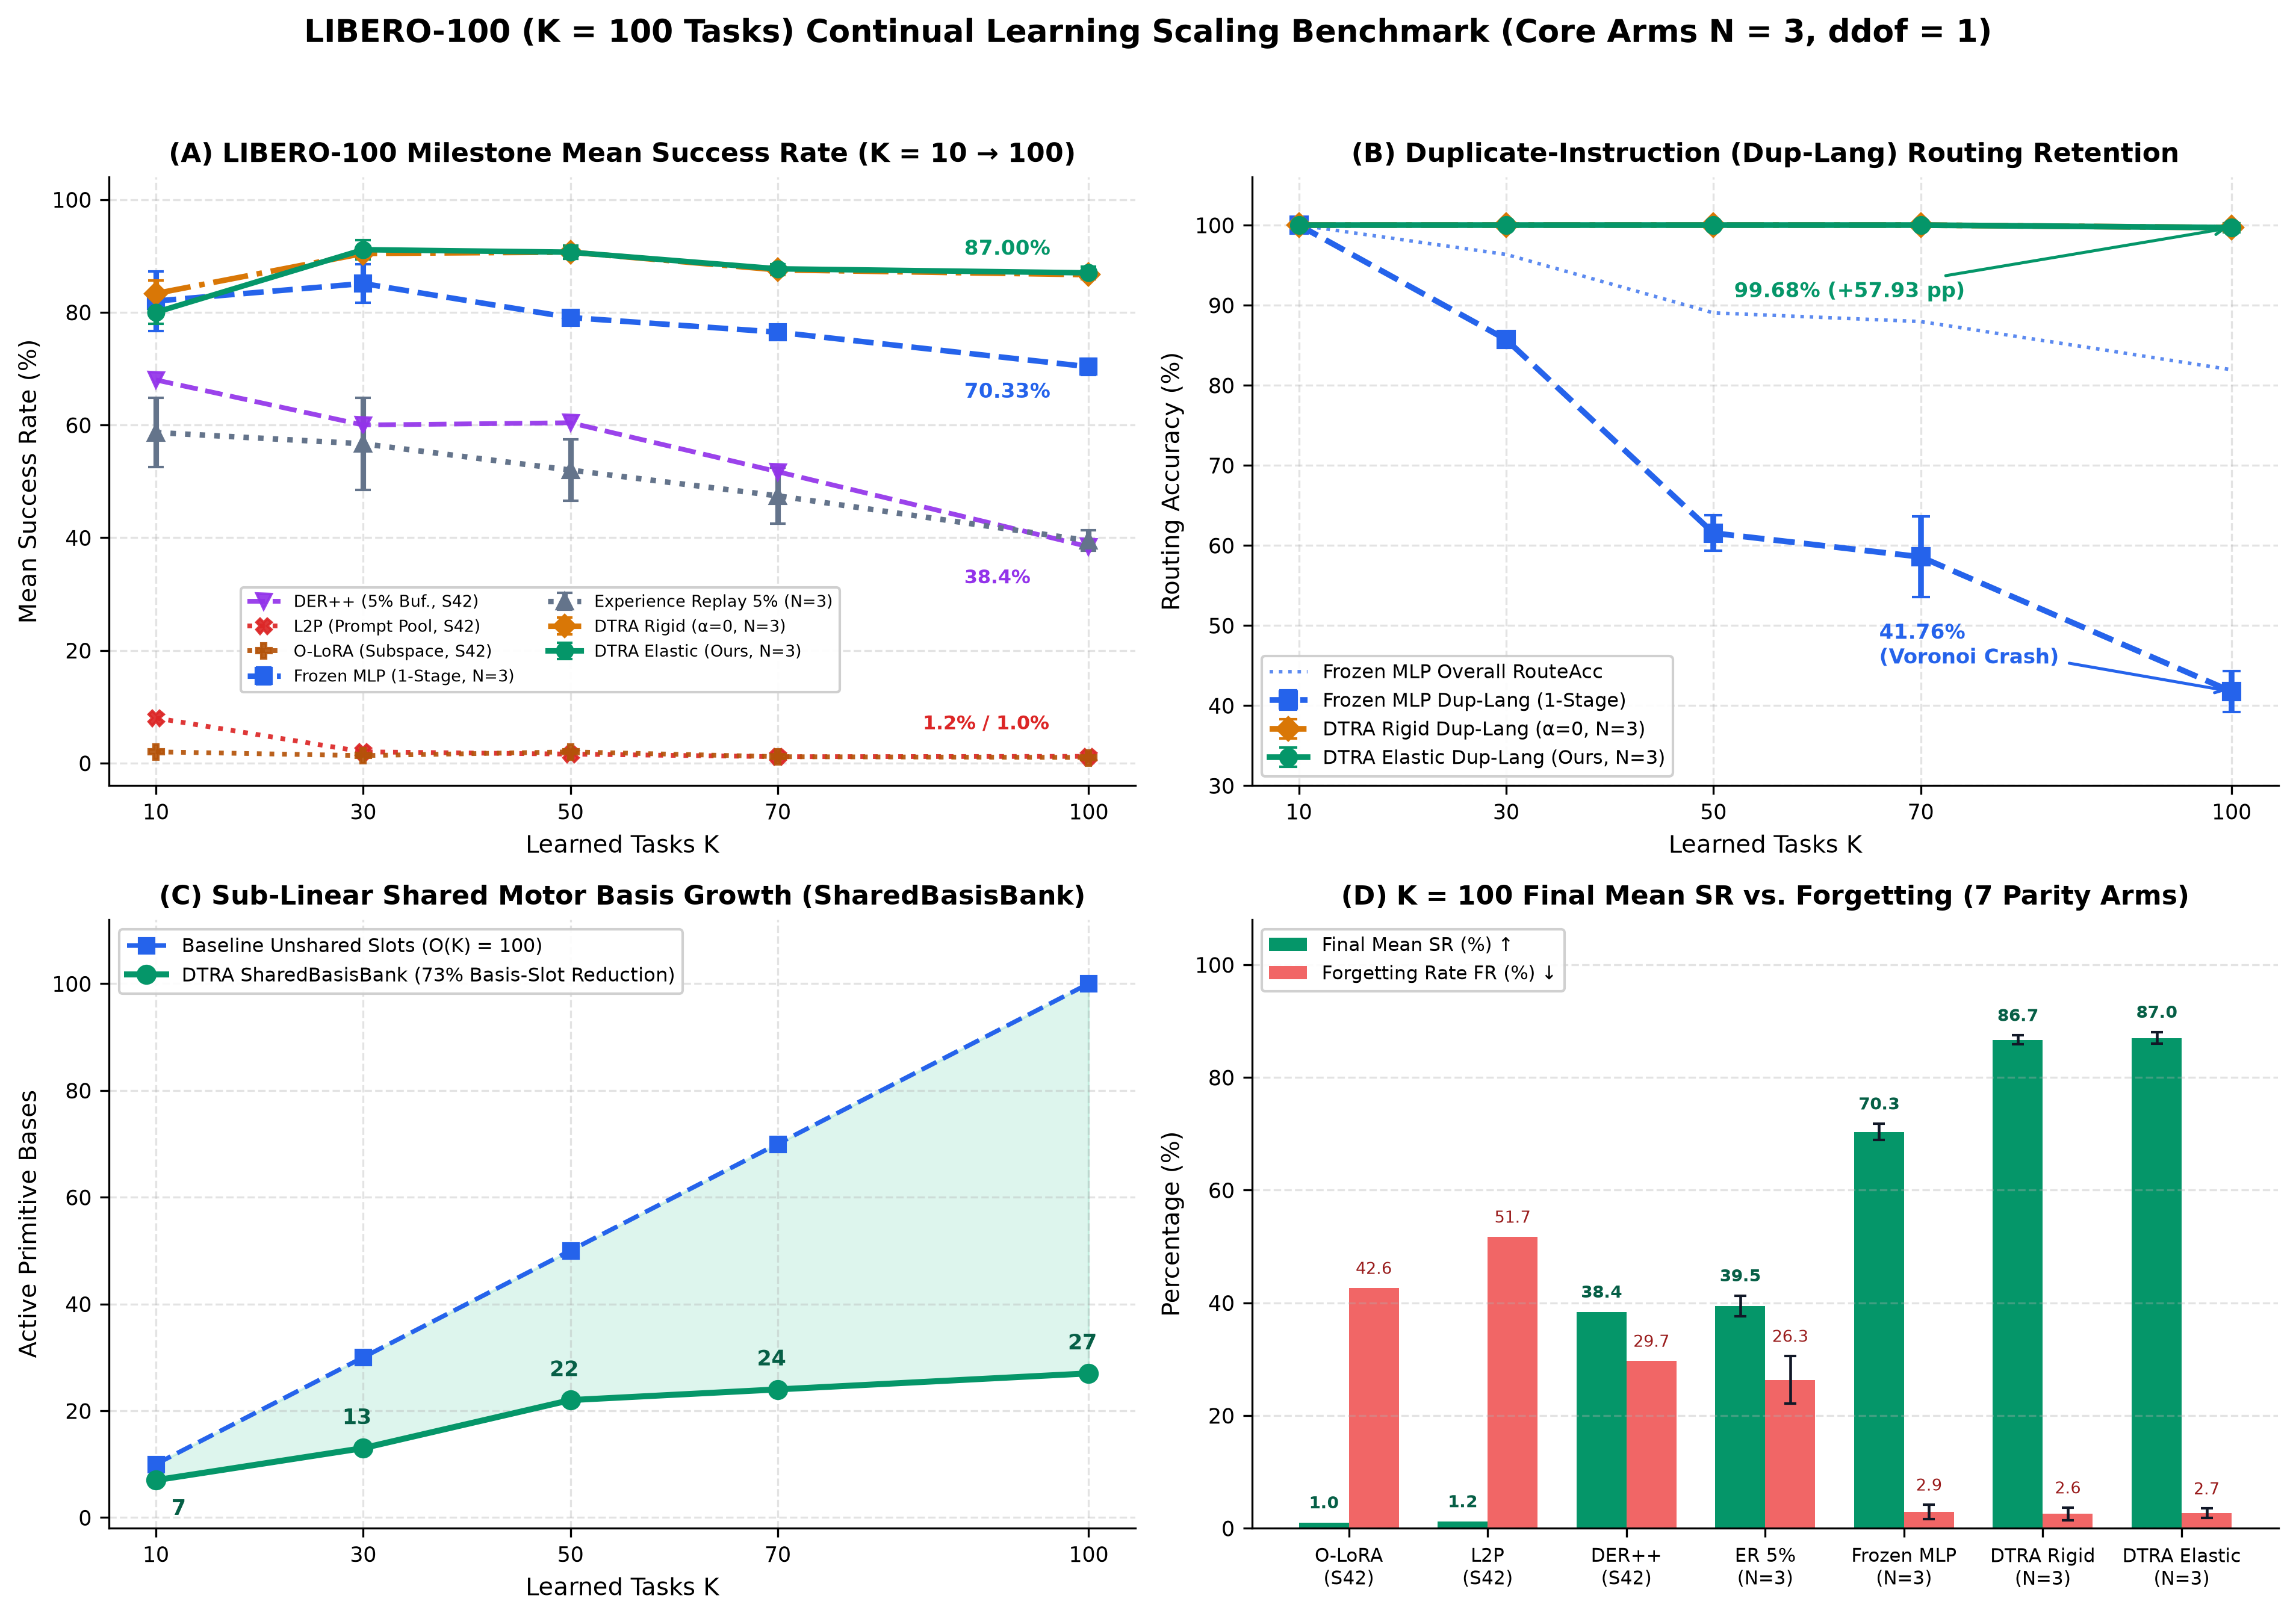
\includegraphics[width=0.86\textwidth]{../../outputs/figures/fig7_libero100_scaling_curves.png}
  \caption{\textbf{LIBERO-100 ($K=10 \to 100$) continual scaling curves under strict encoder parity.} \textbf{(A)} Milestone Mean Success Rate across all 7 parity arms ($K=10\text{--}100$), contrasting DTRA against Frozen MLP, ER~5\%, DER++, L2P, and O-LoRA. \textbf{(B)} Duplicate-Instruction (\texttt{Dup-Lang}) routing retention vs.\ Frozen MLP Voronoi collapse. \textbf{(C)} \texttt{SharedBasisBank} sub-linear saturation ($100 \to 27$ bases, $73\%$ basis-slot reduction). \textbf{(D)} Final $K=100$ Mean SR vs.\ Forgetting Rate across all 7 parity arms (error bars show sample std \texttt{ddof=1} on $N=3$ core arms).}
  \label{fig:libero100_scaling}
\end{figure}


\begin{table}[ht!]
  \centering
  \caption{LIBERO-100 ($K=10 \to 100$, \texttt{libero\_10 + libero\_90}) Continual Scaling SR Trajectory under Strict Encoder Parity ($N=3$ across Seeds~[42, 100, 2026] for all four core arms; Seed~42 for external baselines DER++, L2P, O-LoRA; full multi-metric milestones in Appendix~Table~\ref{tab:libero100_milestones}). Bold marks the highest SR per milestone.}
  \label{tab:libero100_traj}
  \small
  \setlength{\tabcolsep}{3.5pt}
  \begin{tabular}{lccccc}
    \toprule
    \textbf{Arm (Strict Parity)} & \textbf{$K=10$ SR} & \textbf{$K=30$ SR} & \textbf{$K=50$ SR} & \textbf{$K=70$ SR} & \textbf{$K=100$ Final} \\
    \midrule
    Frozen MLP & $82.00 \pm 5.29$\% & $85.11 \pm 3.42$\% & $79.07 \pm 0.61$\% & $76.48 \pm 1.19$\% & $70.33 \pm 1.45$\% \\
    ER 5\% (Replay) & $58.67 \pm 6.11$\% & $56.67 \pm 8.19$\% & $52.00 \pm 5.41$\% & $47.43 \pm 4.98$\% & $39.47 \pm 1.81$\% \\
    DTRA Rigid ($\alpha=0$) & $\mathbf{83.33 \pm 2.31}$\% & $90.44 \pm 1.02$\% & $\mathbf{90.67 \pm 1.15}$\% & $87.52 \pm 0.87$\% & $86.67 \pm 0.81$\% \\
    \textbf{DTRA Elastic (Ours)} & $80.00 \pm 2.00$\% & $\mathbf{91.11 \pm 1.68}$\% & $\mathbf{90.67 \pm 1.22}$\% & $\mathbf{87.71 \pm 0.86}$\% & $\mathbf{87.00 \pm 1.06}$\% \\
    \midrule
    DER++ (5\% Buffer) & 68.00\% & 60.00\% & 60.40\% & 51.71\% & 38.40\% \\
    L2P (Prompt Pool) & 8.00\% & 2.00\% & 1.60\% & 1.14\% & 1.20\% \\
    O-LoRA (Ortho LoRA) & 2.00\% & 1.33\% & 2.00\% & 1.14\% & 1.00\% \\
    \bottomrule
  \end{tabular}
\end{table}

\begin{table}[ht!]
  \centering
  \caption{LIBERO-100 Final $K=100$ Cross-Seed Summary (all rate metrics in \%; Mean $\pm$ Sample Std \texttt{ddof=1}; $N=3$ across Seeds~[42, 100, 2026] for all four core arms; Seed~42 for external baselines DER++, L2P, O-LoRA). Bold numbers mark the best core-arm metric per column (lowest isolated basis count for Bases).}
  \label{tab:libero100_final}
  \fontsize{7.8pt}{9.6pt}\selectfont
  \setlength{\tabcolsep}{2.6pt}
  \begin{tabular}{lcccccccc}
    \toprule
    \textbf{Method} & \textbf{42/100/2026} & \textbf{SR (\%)} & \textbf{FR (\%)$\downarrow$} & \textbf{BWT (\%)$\uparrow$} & \textbf{Rte (\%)$\uparrow$} & \textbf{Dup (\%)} & \textbf{Bases} & \textbf{Lat.(ms)} \\
    \midrule
    Frozen MLP & 72.0/69.6/69.4 & $70.33 \pm 1.45$ & $2.90 \pm 1.28$ & $+0.20 \pm 2.81$ & $81.94 \pm 0.29$ & $41.76 \pm 2.56$ & 100 & $6.46 \pm 0.70$ \\
    ER 5\% (Replay) & 40.2/40.8/37.4 & $39.47 \pm 1.81$ & $26.33 \pm 4.24$ & $-20.00 \pm 3.17$ & --- & --- & 1 & $\mathbf{4.93 \pm 0.72}$ \\
    DTRA Rigid ($\alpha=0$) & 86.2/86.2/87.6 & $86.67 \pm 0.81$ & $\mathbf{2.56 \pm 1.11}$ & $\mathbf{+0.67 \pm 1.35}$ & $\mathbf{99.91 \pm 0.16}$ & $\mathbf{99.68 \pm 0.55}$ & \textbf{27} & $8.70 \pm 1.14$ \\
    \textbf{DTRA Elastic (Ours)} & 87.8/87.4/85.8 & $\mathbf{87.00 \pm 1.06}$ & $2.69 \pm 0.82$ & $+0.20 \pm 0.88$ & $99.90 \pm 0.16$ & $\mathbf{99.68 \pm 0.55}$ & \textbf{27} & $9.55 \pm 0.24$ \\
    \midrule
    DER++ (5\% Buf.) & 38.4/---/--- & 38.40 & 29.70 & $-16.16$ & --- & --- & 1 & 5.49 \\
    L2P (Prompts) & 1.2/---/--- & 1.20 & 51.72 & $-51.72$ & --- & --- & 32 & 7.79 \\
    O-LoRA (Subsp.) & 1.0/---/--- & 1.00 & 42.63 & $-42.63$ & --- & --- & 100 & 7.05 \\
    \bottomrule
  \end{tabular}
\end{table}

\begin{table}[ht!]
  \centering
  \caption{Zero-Retrain Extended Initial-State Verification on Saved $K=100$ LIBERO-100 Checkpoints ($n_{\text{eval}}=20$ initial states/task $\times 100$ tasks $\times 3$ training seeds $= 6{,}000$ rollouts/arm, $12{,}000$ total; Mean $\pm$ Sample Std \texttt{ddof=1}). Brackets show descriptive pooled binomial 95\% Wilson CIs (ignoring task/seed clustering); \texttt{init[5:20]} tests $15$ unseen initial states never evaluated during continual streaming.}
  \label{tab:libero100_neval20}
  \fontsize{7.8pt}{9.6pt}\selectfont
  \setlength{\tabcolsep}{2.6pt}
  \begin{tabular}{lccccc}
    \toprule
    \textbf{Policy ($n=20$)} & \textbf{\texttt{init[0:5]}} & \textbf{Held-Out \texttt{[5:20]} [CI95]} & \textbf{All \texttt{[0:20]} [CI95]} & \textbf{Dup SR (Rte)} & \textbf{Uniq SR} \\
    \midrule
    Frozen MLP & $70.00 \pm 0.92$\% & $68.82 \pm 0.91$\% [67.5, 70.2] & $69.12 \pm 0.90$\% [67.9, 70.3] & 36.33\% (41.80\%) & 83.17\% \\
    \textbf{DTRA Elastic} & $\mathbf{86.40 \pm 1.06}$\% & $\mathbf{84.80 \pm 0.44}$\% \textbf{[83.7, 85.8]} & $\mathbf{85.20 \pm 0.43}$\% \textbf{[84.3, 86.1]} & \textbf{89.06\% (99.94\%)} & \textbf{83.55\%} \\
    \midrule
    \textbf{$\Delta$ (DTRA $-$ MLP)} & \textbf{$+16.40$\,pp} & \textbf{$+15.98$\,pp} & \textbf{$+16.08$\,pp} & \textbf{$+52.72$\,pp ($+58.14$\,pp)} & $+0.38$\,pp \\
    \bottomrule
  \end{tabular}
\end{table}


\textbf{Interpreting Milestone FR/BWT \& Structural Density Crossover.}
At evaluation checkpoints $K \in \{10, 30, 50, 70, 100\}$, Frozen MLP records $70.33 \pm 1.45$\% Mean SR, $41.76 \pm 2.56$\% \texttt{Dup-Lang} routing, and $2.90 \pm 1.28$\% FR. Exact parameter freezing ($\nabla_\theta=0$) is distinct from empirical success-rate retention. Likewise, \texttt{post\_snap\_norm} measures episode-boundary state reset, not parameter drift. DTRA Elastic exhibits an empirical FR of $2.69 \pm 0.82$\% and BWT of $+0.20 \pm 0.88$\%. Notice that on \texttt{Unique-Lang} ($70$ tasks), DTRA Elastic ($83.55\%$) and Frozen MLP ($83.17\%$) are virtually identical; nearly the entire $+16.08\,$pp gain arises from resolving \texttt{Dup-Lang} routing collapse ($89.06\%$ vs.\ $36.33\%$).

% ==========================================================================
\section{Discussion, Scope Boundaries \& Limitations}
\label{sec:discussion}
% ==========================================================================

\subsection{Implementation Scope Boundary: Cell \texorpdfstring{$\to$}{->} Region (v3.0) vs.\ Organ (Future Work / v4.0)}
\textbf{Strict Scope Isolation:} Only the \textbf{Cell} (isolated node with $C^2$ cubic B-Spline knots, No-Encroachment bounds, and $\nabla_\theta=0$ freeze) and single-ring \textbf{Region} ($K=100$ module sharing $27$ primitive bases in \texttt{SharedBasisBank}) are implemented and empirically validated in DTRA~v3.0. All multi-ring \textbf{Organ} scaling architectures, isometric dimension expansion, and object-centric sim/hardware coordinate transport belong strictly to subsequent \textbf{DTRA~v4.0 / Future Work}:
\begin{itemize}[leftmargin=*,itemsep=1.5pt,topsep=2pt]
  \item \textbf{Organ Multi-Ring Coordination (Conceptual / v4.0 Track, $10^4\text{--}10^8$ Tasks):} Coordinating specialized Region rings under hierarchical routing theoretically indexes $100^4 = 10^8$ skills with $O(\log K)$ comparisons ($400$ inner products) and modular portability without saturating one $\mathbb{S}^{63}$ manifold.
  \item \textbf{Isometric Zero-Padding (Proposition~\ref{prop:isometry}, Appendix~\ref{app:proofs}):} Embedding $\mathbf{v} \in \mathbb{S}^{d-1}$ as $[\mathbf{v}; \mathbf{0}] \in \mathbb{S}^{2d-1}$ preserves pairwise inner products and Voronoi boundaries exactly upon future capacity expansion (conceptual property, not implemented in v3.0).
  \item \textbf{Object-Centric Coordinate Transport, Long-Horizon Benchmarks \& Physical Robots (Future Work / v4.0):} Because single-ring Region trajectories use egocentric tabletop frames, extreme object spawn shifts and long-horizon chained manipulation benchmarks such as CALVIN~\cite{mees2022calvin} motivate coupling frozen DTRA bases with object-centric visual anchors (e.g., RGB-D deprojection) and physical robot hardware in future work.
\end{itemize}

\subsection{Structural White-Box Interpretability \& Execution Cost}
DTRA exposes the selected node, shared basis index, routing margin, and episode reset state for inspection (Appendix~\ref{app:whitebox_viz}). Continual registration optimizes newly introduced modules and is distinct from control-time inference. At inference, broad key retrieval scans $K$ entries, followed by conditional 3-modality candidate reranking and decoding of the selected node and basis. The selected decoding core has $O(1)$ cost, while the broad routing scan remains $O(K)$. The measured GPU policy-inference latency is $9.55 \pm 0.24$\,ms at $K=100$; the $1.87\,$ms CPU active-core result concerns the separate $K=1 \to 8$ Meta-World experiment (Figure~\ref{fig:o1_latency}). These timings exclude environment stepping and do not measure registration time.

\subsection{Limitations \& Honest Methodological Caveats}
We highlight six important limitations and methodological caveats verified directly against our implementation:
\begin{enumerate}[leftmargin=*,itemsep=1.5pt,topsep=2pt]
  \item \textbf{Parameter Capacity Ratio ($88{\times}\text{--}108{\times}$) \& Linear $O(K)$ Node Growth:} Although \texttt{SharedBasisBank} reduces knot-basis slots by $73\%$ ($100 \to 27$, $3.81\,$MB), per-task \texttt{LIBEROHypertubeNode} adapters occupy $179.33\,$MB ($97.92\%$ of total policy memory), yielding only a $5.33\%$ total parameter reduction ($183.14\,$MB vs.\ Frozen MLP $151.67\,$MB and monolithic ER/DER++/L2P/O-LoRA heads at $1.70\text{--}2.09\,$MB; Appendix~Table~\ref{tab:libero_resources}; non-parameter buffers add $\sim 9.2\,$MB for DTRA projections/exemplars and $\sim 3.1\,$MB for O-LoRA frozen subspace buffers). True sub-linear total memory requires sharing spatial adapters across tasks (e.g., PackNet or TAIL-style lightweight adapters) in future work.
  \item \textbf{Routing Feature Asymmetry \& Missing \texttt{Frozen MLP + CMC} Ablation:} On LIBERO-100, DTRA's Stage-2 CMC uses a dedicated $6{,}400$-d $4\times 4+2\times 2+\text{DoG}$ visual signature bank plus $\le 96$ cached key-validation exemplars/task (\texttt{\_val\_queries}, $9{,}600$ unit vectors at $K=100$; no raw images/actions), whereas \texttt{Frozen MLP} used 1-stage $2\times 2$ key routing. Because \texttt{Unique-Lang} performance is nearly identical ($83.55\%$ vs.\ $83.17\%$), isolating \texttt{Frozen MLP + No-Encroachment + CMC} remains a key future ablation to decouple router gains from node architecture.
  \item \textbf{External CL Adaptation Caveats (\texttt{L2P} / \texttt{O-LoRA} / \texttt{DER++}):} Our matched-encoder LIBERO-100 external baselines evaluate Seed~42 (complemented by 3-seed Meta-World and an independent A6000 O-LoRA run at $0.40\%$) and represent straightforward non-transformer adaptations rather than upper bounds of those methods: \texttt{L2P} updates its shared MLP head without freezing across tasks (degrading toward naive fine-tuning), \texttt{O-LoRA} freezes its \texttt{SpatialContextAdapter} after Task~0 and saturates the $256$-d orthogonal subspace ($99 \times 8 = 792 > 256$), and \texttt{DER++} uses untuned $\alpha=\beta=0.5$ with $1.70\,$MB capacity (and exhibited cross-run variance of $68.3\text{--}84.2\%$ across separate Meta-World runs). Direct comparison against LIBERO-native \texttt{PackNet}, \texttt{LOTUS}, and \texttt{TAIL} at matched parameter budgets remains future work.
  \item \textbf{Meta-World Clean-vs-OOD Trade-Off, Paraphrase \& Official Test Split:} Our 3-seed Meta-World causal ablation (\texttt{ddof=1}) confirms that disabling Conv4 feature-noise regularization ($p=0,\sigma=0$) lifts DTRA Full from $72.2 \pm 8.3\%$ to $83.1 \pm 6.3\%$ clean SR while preserving $45.0 \pm 6.6\%$ severe OOD SR (whereas adding identical regularization to Frozen MLP yields $90.8 \pm 3.6\%$ clean / $49.2 \pm 10.1\%$ OOD on sparse $K=8$ tasks). Hashed text encoding severely limits free-form paraphrase generalization (3-seed Meta-World paraphrase SR: $26.1 \pm 5.1\%$ for DTRA Full vs.\ $61.1 \pm 5.5\%$ for Frozen MLP), and on the official \texttt{ml1.test\_tasks} split Frozen MLP outperforms DTRA Full ($87.5\%$ vs.\ $75.0\%$).
  \item \textbf{Statistical \& Evaluation Boundaries:} Mid-stream LIBERO-100 checkpoints use $n_{\text{eval}}=5$; final $K=100$ generalization is verified at $n_{\text{eval}}=20$ ($12{,}000$ rollouts, Table~\ref{tab:libero100_neval20}), though pooled Wilson CIs are descriptive binomial intervals that ignore task/seed clustering. \texttt{DTRA Rigid} ($86.67\%$) and \texttt{DTRA Elastic} ($87.00\%$) are statistically indistinguishable at $K=100$.
  \item \textbf{Simulation Scope \& Deterministic Regression:} All experiments run in MuJoCo simulation with distinct-scene \texttt{Dup-Lang} pairs; intra-scene duplicate-instruction disambiguation, multimodal action distributions (where diffusion/CVAE policies excel), and real-world physical robot validation remain essential future work.
\end{enumerate}

% ==========================================================================
\section{Conclusion}
\label{sec:conclusion}
% ==========================================================================

We presented \textbf{DTRA}, a Task-ID-free parameter-isolation framework for continual visuomotor control without raw-demonstration replay. Combining No-Encroachment key refinement (with lightweight 96-vector key-validation exemplars/task), Two-Stage Top-$M$ 3-modality CMC, \texttt{SharedBasisBank} ($100 \to 27$ shared knot bases, $73\%$ basis-slot / $5.33\%$ total parameter reduction), and strict \texttt{AdamW} freeze exclusion ($\nabla_\theta=0$), DTRA Elastic achieves $\mathbf{87.00 \pm 1.06}$\% \textbf{Mean Final SR} (DTRA Rigid: $86.67 \pm 0.81$\%) and $\mathbf{99.68 \pm 0.55}$\% \textbf{Dup-Lang routing} on LIBERO-100 across three seeds---verified at $\mathbf{85.20 \pm 0.43}\%$ ($84.80 \pm 0.44\%$ on $15$ unseen initial states) across $12{,}000$ zero-retrain rollouts ($n_{\text{eval}}=20$)---alongside $0.0\%$ forgetting and $83.1 \pm 6.3\%$ clean / $45.0 \pm 6.6\%$ OOD SR (without feature-noise regularization) on three-seed Meta-World. Transparently reporting both these gains and our architectural/capacity boundaries (linear per-task node memory, routing-feature asymmetry, and hashed-language limits) provides a concrete foundation for future scalable lifelong manipulation.

\clearpage

\begin{thebibliography}{57}
\small
\raggedright
\setlength{\itemsep}{1.1pt}
\setlength{\parskip}{0pt}

\bibitem{vaswani2017attention}
A.~Vaswani, N.~Shazeer, N.~Parmar, J.~Uszkoreit, L.~Jones, A.~N.~Gomez, {\L}.~Kaiser, and I.~Polosukhin, ``Attention is all you need,'' in \emph{Adv.\ Neural Inf.\ Process.\ Syst.\ (NeurIPS)}, vol.~30, 2017.

\bibitem{bommasani2021foundation}
R.~Bommasani et~al., ``On the opportunities and risks of foundation models,'' \texttt{arXiv:2108.07258}, 2021.

\bibitem{brohan2023rt1}
A.~Brohan et~al., ``RT-1: Robotics transformer for real-world control at scale,'' in \emph{Proc.\ Robot.:\ Sci.\ Syst.\ (RSS)}, 2023.

\bibitem{brohan2023rt2}
A.~Brohan et~al., ``RT-2: Vision-language-action models transfer web knowledge to robotic control,'' in \emph{Proc.\ Conf.\ Robot Learn.\ (CoRL)}, 2023.

\bibitem{octo2024}
Octo Model Team, D.~Ghosh, H.~Walke, K.~Pertsch, et~al., ``Octo: An open-source generalist robot policy,'' in \emph{Proc.\ Robot.:\ Sci.\ Syst.\ (RSS)}, 2024.

\bibitem{kim2024openvla}
M.~J.~Kim, K.~Pertsch, S.~Karamcheti, et~al., ``OpenVLA: An open-source vision-language-action model,'' \texttt{arXiv:2406.09246}, 2024.

\bibitem{black2024pi0}
K.~Black et~al., ``$\pi_0$: A vision-language-action flow model for general robot control,'' \texttt{arXiv:2410.24164}, 2024.

\bibitem{zhao2023act}
T.~Z.~Zhao, V.~Kumar, S.~Levine, and C.~Finn, ``Learning fine-grained bimanual manipulation with low-cost hardware,'' in \emph{Proc.\ Robot.:\ Sci.\ Syst.\ (RSS)}, 2023.

\bibitem{chi2023diffusion}
C.~Chi, S.~Feng, Y.~Du, Z.~Xu, E.~Cousineau, B.~Burchfiel, and S.~Song, ``Diffusion policy: Visuomotor policy learning via action diffusion,'' in \emph{Proc.\ Robot.:\ Sci.\ Syst.\ (RSS)}, 2023.

\bibitem{shridhar2022peract}
M.~Shridhar, L.~Manuelli, and D.~Fox, ``Perceiver-Actor: A multi-task transformer for robotic manipulation,'' in \emph{Proc.\ Conf.\ Robot Learn.\ (CoRL)}, 2022.

\bibitem{goyal2023rvt}
A.~Goyal, J.~Xu, Y.~Guo, V.~Blukis, Y.-W.~Chao, and D.~Fox, ``RVT: Robotic view transformer for 3D object manipulation,'' in \emph{Proc.\ Int.\ Conf.\ Mach.\ Learn.\ (ICML)}, 2023.

\bibitem{levine2016end}
S.~Levine, C.~Finn, T.~Darrell, and P.~Abbeel, ``End-to-end training of deep visuomotor policies,'' \emph{J.\ Mach.\ Learn.\ Res.\ (JMLR)}, vol.~17, no.~39, pp.~1--40, 2016.

\bibitem{finn2016deep}
C.~Finn, X.~Y.~Tan, Y.~Duan, T.~Darrell, S.~Levine, and P.~Abbeel, ``Deep spatial autoencoders for visuomotor learning,'' in \emph{Proc.\ IEEE Int.\ Conf.\ Robot.\ Autom.\ (ICRA)}, 2016.

\bibitem{he2016resnet}
K.~He, X.~Zhang, S.~Ren, and J.~Sun, ``Deep residual learning for image recognition,'' in \emph{Proc.\ IEEE/CVF Conf.\ Comput.\ Vis.\ Pattern Recognit.\ (CVPR)}, 2016.

\bibitem{yu2020metaworld}
T.~Yu, D.~Quillen, Z.~He, R.~Julian, A.~Narayan, H.~Shively, A.~Bellathur, K.~Hausman, C.~Finn, and S.~Levine, ``Meta-World: A benchmark and evaluation for multi-task and meta reinforcement learning,'' in \emph{Proc.\ Conf.\ Robot Learn.\ (CoRL)}, 2020.

\bibitem{wolczyk2021continual}
M.~Wo{\l}czyk, M.~Zaj{\k{a}}c, R.~Pascanu, {\L}.~Kuci{\'n}ski, and P.~Mi{\l}o{\'s}, ``Continual World: A robotic benchmark for continual reinforcement learning,'' in \emph{Adv.\ Neural Inf.\ Process.\ Syst.\ (NeurIPS)}, vol.~34, 2021.

\bibitem{liu2023libero}
B.~Liu, Y.~Zhu, C.~Gao, Y.~Feng, Q.~Liu, Y.~Zhu, and P.~Stone, ``LIBERO: Benchmarking knowledge transfer for lifelong robot learning,'' in \emph{Adv.\ Neural Inf.\ Process.\ Syst.\ (NeurIPS Datasets and Benchmarks Track)}, 2023.

\bibitem{mees2022calvin}
O.~Mees, L.~Hermann, E.~Rosete-Beas, and W.~Burgard, ``CALVIN: A benchmark for language-conditioned policy learning for long-horizon robot manipulation tasks,'' \emph{IEEE Robot.\ Autom.\ Lett.\ (RA-L)}, vol.~7, no.~3, pp.~7327--7334, 2022.

\bibitem{mccloskey1989catastrophic}
M.~McCloskey and N.~J.~Cohen, ``Catastrophic interference in connectionist networks: The sequential learning problem,'' \emph{Psychol.\ Learn.\ Motiv.}, vol.~24, pp.~109--165, 1989.

\bibitem{french1999catastrophic}
R.~M.~French, ``Catastrophic forgetting in connectionist networks,'' \emph{Trends Cogn.\ Sci.}, vol.~3, no.~4, pp.~128--135, 1999.

\bibitem{parisi2019continual}
G.~I.~Parisi, R.~Kemker, J.~L.~Part, C.~Kanan, and S.~Wermter, ``Continual lifelong learning with neural networks: A review,'' \emph{Neural Netw.}, vol.~113, pp.~54--71, 2019.

\bibitem{kirkpatrick2017ewc}
J.~Kirkpatrick et~al., ``Overcoming catastrophic forgetting in neural networks,'' \emph{Proc.\ Natl.\ Acad.\ Sci.\ (PNAS)}, vol.~114, no.~13, pp.~3521--3526, 2017.

\bibitem{zenke2017si}
F.~Zenke, B.~Poole, and S.~Ganguli, ``Continual learning through synaptic intelligence,'' in \emph{Proc.\ Int.\ Conf.\ Mach.\ Learn.\ (ICML)}, 2017.

\bibitem{aljundi2018mas}
R.~Aljundi, F.~Babiloni, M.~Elhoseiny, M.~Rohrbach, and T.~Tuytelaars, ``Memory aware synapses: Learning what (not) to forget,'' in \emph{Proc.\ Eur.\ Conf.\ Comput.\ Vis.\ (ECCV)}, 2018.

\bibitem{chaudhry2018rwalk}
A.~Chaudhry, P.~K.~Dokania, T.~Ajanthan, and P.~H.~S.~Torr, ``Riemannian walk for incremental learning: Understanding forgetting and intransigence,'' in \emph{Proc.\ Eur.\ Conf.\ Comput.\ Vis.\ (ECCV)}, 2018.

\bibitem{lopezpaz2017gem}
D.~Lopez-Paz and M.~Ranzato, ``Gradient episodic memory for continual learning,'' in \emph{Adv.\ Neural Inf.\ Process.\ Syst.\ (NeurIPS)}, 2017.

\bibitem{chaudhry2019agem}
A.~Chaudhry, M.~Ranzato, M.~Rohrbach, and M.~Elhoseiny, ``Efficient lifelong learning with A-GEM,'' in \emph{Proc.\ Int.\ Conf.\ Learn.\ Represent.\ (ICLR)}, 2019.

\bibitem{rolnick2019clear}
D.~Rolnick, A.~Ahuja, J.~Schwarz, T.~P.~Lillicrap, and G.~Wayne, ``Experience replay for continual learning,'' in \emph{Adv.\ Neural Inf.\ Process.\ Syst.\ (NeurIPS)}, 2019.

\bibitem{buzzega2020der}
P.~Buzzega, M.~Boschini, A.~Porrello, D.~Abati, and S.~Calderara, ``Dark experience for general continual learning: a strong, simple baseline,'' in \emph{Adv.\ Neural Inf.\ Process.\ Syst.\ (NeurIPS)}, 2020.

\bibitem{rusu2016pnn}
A.~A.~Rusu, N.~C.~Rabinowitz, G.~Desjardins, H.~Soyer, J.~Kirkpatrick, K.~Kavukcuoglu, R.~Pascanu, and R.~Hadsell, ``Progressive neural networks,'' \texttt{arXiv:1606.04671}, 2016.

\bibitem{mallya2018packnet}
A.~Mallya and S.~Lazebnik, ``PackNet: Adding multiple tasks to a single network by iterative pruning,'' in \emph{Proc.\ IEEE/CVF Conf.\ Comput.\ Vis.\ Pattern Recognit.\ (CVPR)}, 2018.

\bibitem{serra2018hat}
J.~Serr{\`a}, D.~Sur{\'\i}s, M.~Miron, and A.~Karatzoglou, ``Overcoming catastrophic forgetting with hard attention to the task,'' in \emph{Proc.\ Int.\ Conf.\ Mach.\ Learn.\ (ICML)}, 2018.

\bibitem{wang2022l2p}
Z.~Wang et~al., ``Learning to prompt for continual learning,'' in \emph{Proc.\ IEEE/CVF Conf.\ Comput.\ Vis.\ Pattern Recognit.\ (CVPR)}, 2022.

\bibitem{wang2022dualprompt}
Z.~Wang, Z.~Zhang, S.~Ebrahimi, R.~Sun, H.~Zhang, C.-Y.~Lee, X.~Ren, G.~Su, V.~Perot, J.~Dy, and T.~Pfister, ``DualPrompt: Complementary prompting for rehearsal-free continual learning,'' in \emph{Proc.\ Eur.\ Conf.\ Comput.\ Vis.\ (ECCV)}, 2022.

\bibitem{smith2023coda}
J.~S.~Smith, L.~Karlinsky, V.~Gutta, P.~Cascante-Bonilla, D.~Kim, A.~Arbelle, R.~Panda, R.~Feris, and Z.~Kira, ``CODA-Prompt: COntinual Decomposed Attention-based Prompting for rehearsal-free continual learning,'' in \emph{Proc.\ IEEE/CVF Conf.\ Comput.\ Vis.\ Pattern Recognit.\ (CVPR)}, 2023.

\bibitem{hu2022lora}
E.~J.~Hu, Y.~Shen, P.~Wallis, Z.~Allen-Zhu, Y.~Li, S.~Wang, L.~Wang, and W.~Chen, ``LoRA: Low-rank adaptation of large language models,'' in \emph{Proc.\ Int.\ Conf.\ Learn.\ Represent.\ (ICLR)}, 2022.

\bibitem{saha2021gpm}
G.~Saha, I.~Garg, and K.~Roy, ``Gradient projection memory for continual learning,'' in \emph{Proc.\ Int.\ Conf.\ Learn.\ Represent.\ (ICLR)}, 2021.

\bibitem{wang2023olora}
X.~Wang, T.~Chen, Q.~Ge, H.~Xia, R.~Bao, R.~Zheng, Q.~Zhang, T.~Gui, and X.~Huang, ``Orthogonal subspace learning for language model continual learning,'' in \emph{Findings of EMNLP}, 2023.

\bibitem{liang2024inflora}
Y.-S.~Liang and W.-J.~Li, ``InfLoRA: Interference-free low-rank adaptation for continual learning,'' in \emph{Proc.\ IEEE/CVF Conf.\ Comput.\ Vis.\ Pattern Recognit.\ (CVPR)}, 2024.

\bibitem{parsa2026seqlora}
J.~Parsa, E.~Simsar, A.~Joudaki, T.~Hofmann, and A.~M.~H.~Teixeira, ``SeqLoRA: Bilevel orthogonal adaptation for continual multi-concept generation,'' \texttt{arXiv:2605.22743}, 2026.

\bibitem{luo2026keeplora}
M.-L.~Luo, Z.-H.~Zhou, Y.-L.~Zhang, Y.~Wan, M.-L.~Zhang, and T.~Wei, ``KeepLoRA: Continual learning with residual gradient adaptation,'' in \emph{Proc.\ Int.\ Conf.\ Learn.\ Represent.\ (ICLR)} (\texttt{arXiv:2601.19659}), 2026.

\bibitem{wang2026orthoskill}
J.~Wang, Z.~Fang, Q.~Shi, and Y.~Zhou, ``OrthoSkillVLA: Continual skill learning via gradient-informed skill subspace adaptation,'' \texttt{arXiv:2608.19589}, 2026.

\bibitem{shrivastava2026sambar}
A.~Shrivastava, X.~Zhou, H.~Zhao, Z.~Chen, and N.~Mehr, ``SAMBAR: Selective anchoring via method of multipliers for balanced knowledge acquisition and retention in vision-language-action models,'' \texttt{arXiv:2609.32108}, 2026.

\bibitem{fang2026r2wam}
K.~Fang, H.~Liu, C.~Shi, Y.~Zhou, H.~Zhu, M.~Guo, J.~Song, and L.~Gao, ``Data-free continual learning for world action model with rectified generative replay,'' \texttt{arXiv:2610.18038}, 2026.

\bibitem{chen2026opr}
Y.~Chen, T.~Zhu, M.~Zhang, X.~Chen, J.~Huang, D.~Xu, and Y.~Wang, ``On-policy replay for continual supervised fine-tuning,'' \texttt{arXiv:2605.29495}, 2026.

\bibitem{zhang2026composecl}
Z.~Zhang, A.~Zhang, D.~Khashabi, and T.~Shu, ``Continual learning mechanisms compose for long-horizon memorization,'' \texttt{arXiv:2609.06986}, 2026.

\bibitem{ijspeert2013dmp}
A.~J.~Ijspeert, J.~Nakanishi, H.~Hoffmann, P.~Pastor, and S.~Schaal, ``Dynamical movement primitives: Learning attractor models for motor behaviors,'' \emph{Neural Comput.}, vol.~25, no.~2, pp.~328--373, 2013.

\bibitem{paraschos2013promp}
A.~Paraschos, C.~Daniel, J.~Peters, and G.~Neumann, ``Probabilistic movement primitives,'' in \emph{Adv.\ Neural Inf.\ Process.\ Syst.\ (NeurIPS)}, vol.~26, 2013.

\bibitem{piegl1997nurbs}
L.~Piegl and W.~Tiller, \emph{The NURBS Book}, 2nd~ed.\hskip 1em plus 0.5em minus 0.4em\relax Springer, 1997.

\bibitem{deboor1978splines}
C.~de~Boor, \emph{A Practical Guide to Splines}.\hskip 1em plus 0.5em minus 0.4em\relax Springer-Verlag, 1978.

\bibitem{deng2019arcface}
J.~Deng, J.~Guo, N.~Xue, and S.~Zafeiriou, ``ArcFace: Additive angular margin loss for deep face recognition,'' in \emph{Proc.\ IEEE/CVF Conf.\ Comput.\ Vis.\ Pattern Recognit.\ (CVPR)}, 2019.

\bibitem{kanerva2009hdc}
P.~Kanerva, ``Hyperdimensional computing: An introduction to computing in distributed representation with high-dimensional random vectors,'' \emph{Cogn.\ Comput.}, vol.~1, no.~2, pp.~139--159, 2009.

\bibitem{papyan2020neural}
V.~Papyan, X.~Y.~Han, and D.~L.~Donoho, ``Prevalence of neural collapse during the terminal phase of deep learning training,'' \emph{Proc.\ Natl.\ Acad.\ Sci.\ (PNAS)}, vol.~117, no.~40, pp.~24652--24663, 2020.

\bibitem{zhu2022buds}
Y.~Zhu, P.~Stone, and Y.~Zhu, ``Bottom-up skill discovery from unsegmented demonstrations for long-horizon robot manipulation,'' \emph{IEEE Robot.\ Autom.\ Lett.\ (RA-L)}, vol.~7, no.~2, pp.~4126--4133, 2022.

\bibitem{wan2024lotus}
W.~Wan, Y.~Zhu, R.~Shah, and Y.~Zhu, ``LOTUS: Continual imitation learning for robot manipulation through unsupervised skill discovery,'' in \emph{Proc.\ IEEE Int.\ Conf.\ Robot.\ Autom.\ (ICRA)}, 2024.

\bibitem{liu2024tail}
Z.~Liu, J.~Zhang, K.~Asadi, Y.~Liu, D.~Zhao, S.~Sabach, and R.~Fakoor, ``TAIL: Task-specific adapters for imitation learning with large pretrained models,'' in \emph{Proc.\ Int.\ Conf.\ Learn.\ Represent.\ (ICLR)}, 2024.

\bibitem{son2026abkvla}
S.~Son, ``ABK-VLA: Task-ID-free continual visuomotor policy learning via autonomous B-Spline knot compression and visual prototype routing,'' \emph{Zenodo Preprint}, v1.1.3 DOI: \texttt{10.5281/zenodo.24212130} (Concept DOI: \texttt{10.5281/zenodo.24208544}), Nov.\ 2026. Repository: \url{https://github.com/5Color/abk-vla}.

\end{thebibliography}


\clearpage
\appendix

\section{Implementation Invariants \& Geometric Properties}
\label{app:proofs}

This appendix records three verification properties underlying the mechanisms in Sections~\ref{sec:method} and~\ref{sec:discussion}: exact zero optimizer drift under \texttt{AdamW} parameter-group exclusion (Proposition~\ref{prop:zero_drift}), standard clamped cubic B-Spline within-chunk continuity and output perturbation bounds (Proposition~\ref{prop:bspline}), and the conceptual isometric zero-padding property noted for future capacity expansion (Proposition~\ref{prop:isometry}). We frame these explicitly as implementation invariants and standard mathematical properties rather than novel theorems.

\subsection{Zero Optimizer Drift Under Consolidated Parameter Exclusion}
\begin{proposition}[Exact Zero Optimizer Drift \& Episode State Reset]
\label{prop:zero_drift}
Let $\Theta_{\text{frozen}}^{(k)} = \{\mathbf{k}_j, \mathbf{B}_{b_j}, \mathbf{W}_{\text{node},j}\}_{j=1}^{k}$ denote consolidated keys, shared motor bases in \texttt{SharedBasisBank}, and prior node weights after mastering task $T_k$. Under DTRA registration:
\begin{enumerate}[leftmargin=*,itemsep=2pt]
  \item \textbf{Zero Optimizer Drift ($L_\infty = 0.0$):} For any subsequent task curriculum $T_{k+1}, \dots, T_K$ trained with decoupled weight decay \texttt{AdamW} ($\lambda > 0$), $\|\Theta_{\text{frozen}}^{(k)}(T_K) - \Theta_{\text{frozen}}^{(k)}(T_k)\|_\infty = 0.0$ holds identically.
  \item \textbf{Deterministic Episode-Boundary Reset:} Calling \texttt{episode\_snap\_back()} prior to $t=0$ clears active routing inertia (\texttt{prev\_selected}, \texttt{prev\_act\_vec}) and diagnostic deformation buffers to exact $0.0000$, preventing inter-episode state carryover.
\end{enumerate}
\end{proposition}

\begin{proof}
(1) Standard \texttt{AdamW} updates obey $\theta_{s+1} = (1 - \eta\lambda)\theta_s - \eta \hat{m}_s / (\sqrt{\hat{v}_s} + \epsilon)$. Even when $\nabla_\theta\mathcal{L} = \mathbf{0}$, retaining $\theta_s$ inside an optimizer parameter group applies silent exponential decay $(1 - \eta\lambda)^S \theta_0 \neq \theta_0$. DTRA sets \texttt{requires\_grad=False} on $\Theta_{\text{frozen}}^{(k)}$ and instantiates each task's \texttt{AdamW} optimizer exclusively over newly created active parameters ($\Theta_{\text{frozen}}^{(k)} \cap \text{param\_groups}(\texttt{AdamW}) = \emptyset$), so $\theta_{s+1} = \theta_s$ identically in IEEE-754 arithmetic. (2) Explicit zero-reinitialization of routing inertia and diagnostic buffers at episode reset guarantees identical initial internal state at every $t=0$. Note that parameter stability (1) is distinct from empirical closed-loop success-rate forgetting, which can still be non-zero due to routing boundary changes or rollout stochasticity.
\end{proof}

\subsection{Clamped \texorpdfstring{$C^2$}{C2} Cubic B-Spline Continuity \& Perturbation Bound}
\begin{proposition}[Within-Chunk $C^2$ Continuity and Convex-Hull Perturbation Bound]
\label{prop:bspline}
Let the clamped uniform degree $p=3$ knot vector $U = \{0, 0, 0, 0, u_4, \dots, u_{N_{\text{cp}}-1}, 1, 1, 1, 1\}$ have $N_{\text{cp}}$ control points $\mathbf{P} \in \mathbb{R}^{N_{\text{cp}} \times d_a}$ ($N_{\text{cp}}=8$ on LIBERO-100; $N_{\text{cp}}=6$ on Meta-World), evaluated at $\tau_h = h / (H-1)$ for $h = 0, \dots, H-1$ ($H=16$). By standard spline properties~\cite{deboor1978splines,piegl1997nurbs}:
\begin{enumerate}[leftmargin=*,itemsep=2pt]
  \item Every synthesized chunk $\mathbf{a}(\tau) = \sum_{n=0}^{N_{\text{cp}}-1} B_{n,3}(\tau)\,\mathbf{p}_n$ satisfies endpoint clamping ($\mathbf{a}(0) = \mathbf{p}_0$, $\mathbf{a}(1) = \mathbf{p}_{N_{\text{cp}}-1}$) and $C^2$ continuity at all interior knots.
  \item By non-negativity ($B_{n,3}(\tau) \ge 0$) and partition of unity ($\sum_{n=0}^{N_{\text{cp}}-1} B_{n,3}(\tau) \equiv 1$), any knot perturbation $\|\delta\mathbf{P}\|_\infty \le \epsilon$ obeys $\sup_{\tau \in [0,1]} \|\delta\mathbf{a}(\tau)\|_\infty \le \epsilon$ within a single chunk.
\end{enumerate}
\end{proposition}

\begin{proof}
By Cox--de~Boor recursion with multiplicity-$4$ boundary knots and simple interior knots ($m_j=1$), $\mathbf{a}(\tau)$ is $C^{p-m_j}=C^2$ across interior transitions and satisfies $B_{n,3}(\tau) \ge 0$, $\sum_{n=0}^{N_{\text{cp}}-1} B_{n,3}(\tau) = 1$. H\"older's inequality immediately yields $\left\| \sum_{n} B_{n,3}(\tau)\, \delta\mathbf{p}_n \right\|_\infty \le (\sum_n |B_{n,3}(\tau)|)\max_n \|\delta\mathbf{p}_n\|_\infty = \|\delta\mathbf{P}\|_\infty \le \epsilon$. Replanning-boundary smoothness across consecutive chunks and physical actuator torque limits are outside this single-chunk bound.
\end{proof}

\subsection{Conceptual Isometric Zero-Padding Property (Future Work)}
\begin{proposition}[Isometric Zero-Padding Inner-Product Preservation]
\label{prop:isometry}
For unit vectors $\{\mu_j, \mathbf{k}_j\}_{j=1}^K \subset \mathbb{S}^{d-1}$, the zero-padding map $\Phi_d^{D}(\mathbf{v}) = [\mathbf{v}; \mathbf{0}_{D-d}] \in \mathbb{S}^{D-1}$ ($D > d$) preserves all norms and pairwise inner products identically ($\langle \Phi_d^D(\mathbf{u}), \Phi_d^D(\mathbf{v}) \rangle = \langle \mathbf{u}, \mathbf{v} \rangle$), thereby preserving existing spherical Voronoi partitions and No-Encroachment margins $\langle \mu_j, \mathbf{k}_i \rangle \le s_{jj} - m_{\text{safe}}$ without distortion. This property is noted solely as a conceptual design primitive for future capacity expansion and is not implemented in DTRA~v3.0.
\end{proposition}


\subsection{Asymptotic Dispatch Complexity \& \texorpdfstring{$O(1)$}{O(1)} Active Core Scaling}
Because inactive cells and unreferenced motor bases remain idle behind gated Top-$M$ retrieval, active action decoding evaluates strictly one selected cell and its bound primitive slot $\mathbf{B}_{b^*}$ regardless of historical task count $K$. As verified empirically in Figure~\ref{fig:o1_latency}, single-thread CPU active execution stays flat at $1.87\,$ms across $K=1 \to 8$, whereas naive residual chaining grows monotonically with depth.

\begin{figure}[ht!]
  \centering
  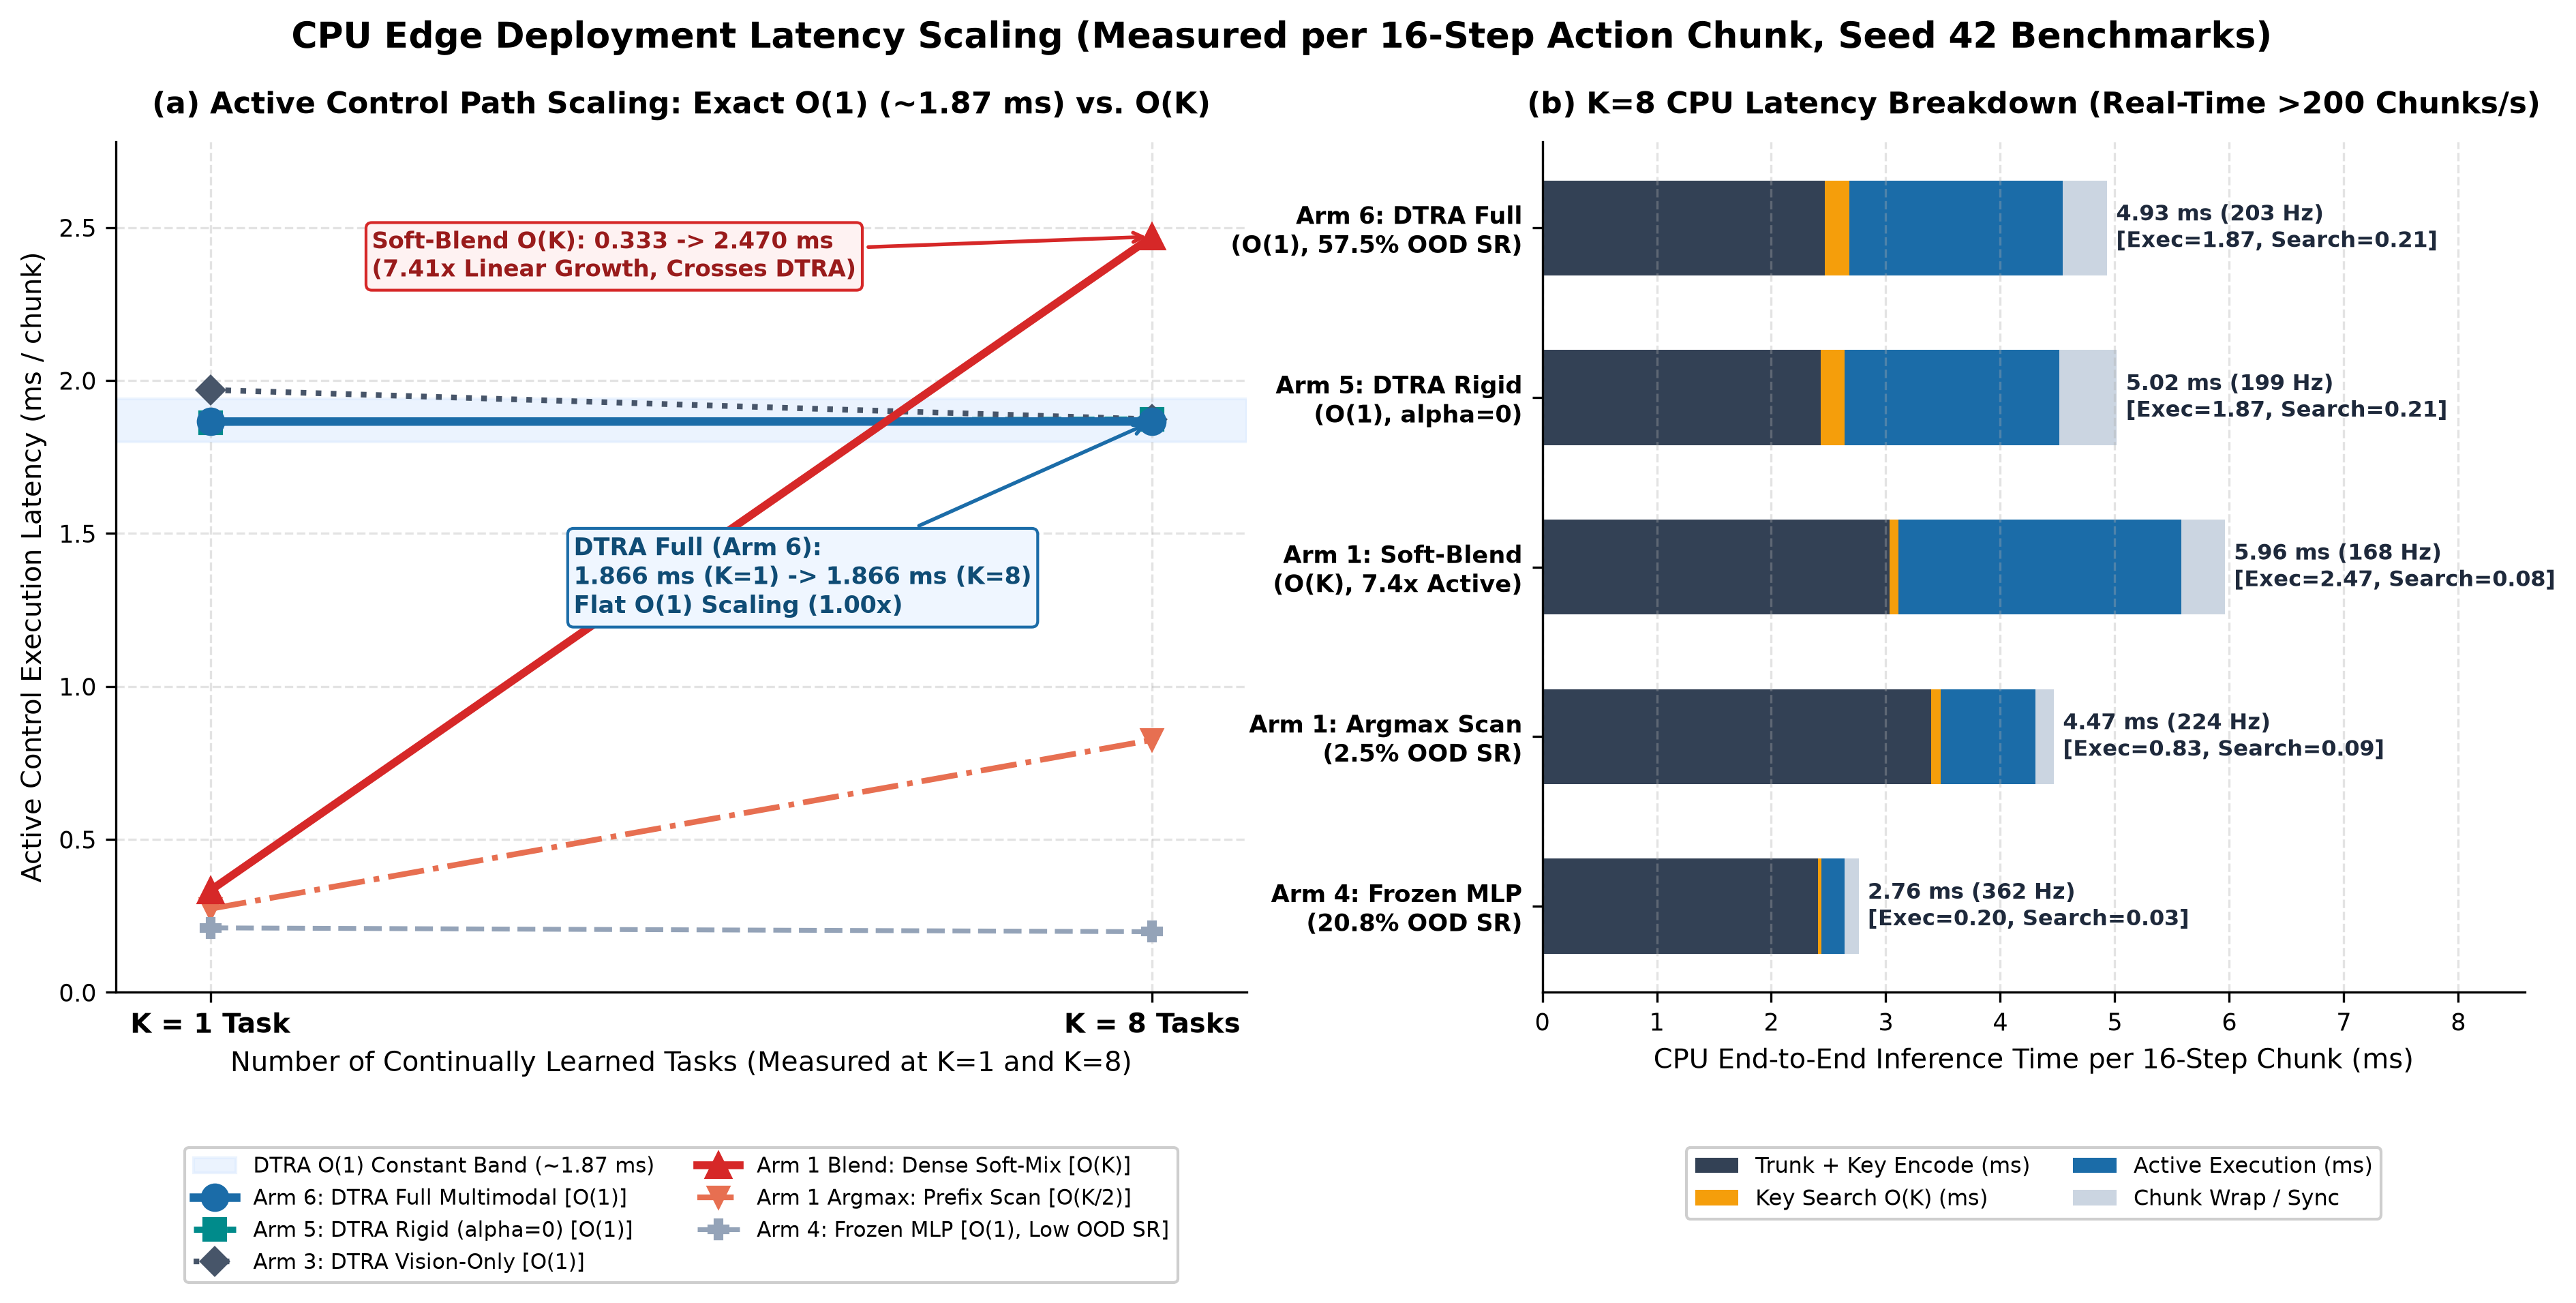
\includegraphics[width=0.82\textwidth]{../../outputs/figures/fig5_o1_latency_scaling.png}
  \caption{\textbf{Constant $O(1)$ Active Core Execution Latency vs.\ $O(K)$ Residual Chaining (Meta-World, Seed~42).} Active DTRA computation remains invariant across increasing library size ($1.87\,$ms on CPU from $K=1 \to 8$), avoiding linear latency degradation.}
  \label{fig:o1_latency}
\end{figure}


\clearpage
\section{LIBERO-100 Detailed Milestone Splits, Stratified Scenes \& Reproducibility}
\label{app:libero_details}

Table~\ref{tab:seed_registry} documents the exact provenance of every LIBERO-100 ($K=100$) JSON artifact bound to this manuscript, and Table~\ref{tab:libero100_milestones} provides the complete five-checkpoint evaluation trajectory across all parity arms and external continual baselines. All summary tables strictly parse finalized JSON artifacts ($N=3$ across Seeds~[42, 100, 2026] for all four core arms; Seed~42 for external baselines \texttt{DER++}, \texttt{L2P}, and \texttt{O-LoRA}; plus $12{,}000$-rollout $n_{\text{eval}}=20$ zero-retrain verification on saved $K=100$ checkpoints).

\begin{table}[ht!]
  \centering
  \caption{Provenance and verification registry of LIBERO-100 ($K=100$) multi-seed, external baseline, and $n_{\text{eval}}=20$ artifacts.}
  \label{tab:seed_registry}
  \tblfont
  \setlength{\tabcolsep}{3.5pt}
  \begin{tabular}{>{\raggedright\arraybackslash}p{0.11\textwidth}>{\raggedright\arraybackslash}p{0.16\textwidth}>{\raggedright\arraybackslash}p{0.29\textwidth}>{\raggedright\arraybackslash}p{0.37\textwidth}}
    \toprule
    \textbf{Artifact} & \textbf{Status} & \textbf{Completed Coverage} & \textbf{Verified Local Artifact Path} \\
    \midrule
    Seed~42 & Verified (\texttt{COMPLETED}) & 4 Arms (\texttt{arm\_\allowbreak frozen\_\allowbreak mlp, arm\_\allowbreak dtra\_\allowbreak elastic, arm\_\allowbreak dtra\_\allowbreak rigid, arm\_\allowbreak er\_\allowbreak 5pct}) & \texttt{benchmark\_\allowbreak dtra\_\allowbreak libero\_\allowbreak 10\_\allowbreak libero\_\allowbreak 90\_\allowbreak k100\_\allowbreak seed42\_\allowbreak locked.json} \\
    Seed~100 & Verified (\texttt{COMPLETED}) & 4 Arms (\texttt{arm\_\allowbreak frozen\_\allowbreak mlp, arm\_\allowbreak dtra\_\allowbreak elastic, arm\_\allowbreak dtra\_\allowbreak rigid, arm\_\allowbreak er\_\allowbreak 5pct}) & \texttt{benchmark\_\allowbreak dtra\_\allowbreak libero\_\allowbreak 10\_\allowbreak libero\_\allowbreak 90\_\allowbreak k100\_\allowbreak seed100\_\allowbreak locked.json} \\
    Seed~2026 & Verified (\texttt{COMPLETED}) & 4 Arms (\texttt{arm\_\allowbreak frozen\_\allowbreak mlp, arm\_\allowbreak dtra\_\allowbreak elastic, arm\_\allowbreak dtra\_\allowbreak rigid, arm\_\allowbreak er\_\allowbreak 5pct}) & \texttt{benchmark\_\allowbreak dtra\_\allowbreak libero\_\allowbreak 10\_\allowbreak libero\_\allowbreak 90\_\allowbreak k100\_\allowbreak seed2026\_\allowbreak locked.json + benchmark\_\allowbreak dtra\_\allowbreak libero\_\allowbreak k100\_\allowbreak seed2026\_\allowbreak rigid.json + benchmark\_\allowbreak dtra\_\allowbreak libero\_\allowbreak k100\_\allowbreak seed2026\_\allowbreak er5.json} \\
    Ext.~CL (S42) & Verified (\texttt{COMPLETED}) & 3 Arms (\texttt{arm\_\allowbreak derpp, arm\_\allowbreak l2p, arm\_\allowbreak olora}) & \texttt{benchmark\_\allowbreak dtra\_\allowbreak libero\_\allowbreak v31\_\allowbreak ext\_\allowbreak cl\_\allowbreak k100\_\allowbreak seed42.json} \\
    Ext.~$n=20$ & Verified (\texttt{COMPLETED}) & 6 Runs ($12{,}000$ rollouts, 3 seeds $\times$ 2 arms) & \texttt{eval\_\allowbreak libero100\_\allowbreak extended\_\allowbreak neval20.json} \\
    \bottomrule
  \end{tabular}
\end{table}


\begin{table}[ht!]
  \centering
  \caption{Full LIBERO-100 ($K=10 \to 100$) Multi-Metric Continual Milestones under Strict Encoder Parity ($N=3$ across Seeds~[42, 100, 2026] for all four core arms; Seed~42 for external baselines DER++, L2P, O-LoRA).}
  \label{tab:libero100_milestones}
  \fontsize{8.0pt}{9.8pt}\selectfont
  \setlength{\tabcolsep}{2.5pt}
  \begin{tabular}{llcccccc}
    \toprule
    \textbf{$K$} & \textbf{Arm (Strict Parity)} & \textbf{Mean SR $\uparrow$} & \textbf{FR $\downarrow$} & \textbf{BWT $\uparrow$} & \textbf{Route $\uparrow$} & \textbf{Dup-Lang $\uparrow$} & \textbf{Bases} \\
    \midrule
    $K=10$ & Frozen MLP & $82.00 \pm 5.29$\% & $2.96 \pm 3.39$\% & $-2.96 \pm 3.39$\% & $\mathbf{100.00 \pm 0.00}$\% & $\mathbf{100.00 \pm 0.00}$\% & 10 \\
     & ER 5\% (Replay) & $58.67 \pm 6.11$\% & $25.19 \pm 8.41$\% & $-25.19 \pm 8.41$\% & --- & --- & 1 \\
     & DTRA Rigid ($\alpha=0$) & $\mathbf{83.33 \pm 2.31}$\% & $2.96 \pm 1.28$\% & $+0.74 \pm 3.39$\% & $\mathbf{100.00 \pm 0.00}$\% & $\mathbf{100.00 \pm 0.00}$\% & 7 \\
     & \textbf{DTRA Elastic (Ours)} & $80.00 \pm 2.00$\% & $2.96 \pm 1.28$\% & $-1.48 \pm 3.39$\% & $\mathbf{100.00 \pm 0.00}$\% & $\mathbf{100.00 \pm 0.00}$\% & 7 \\
    & DER++ (5\% Buf., S42) & 68.00\% & 28.89\% & $-28.89$\% & --- & --- & 1 \\
    & L2P (Prompts, S42) & 8.00\% & 80.00\% & $-80.00$\% & --- & --- & 32 \\
    & O-LoRA (Subsp., S42) & 2.00\% & 31.11\% & $-31.11$\% & --- & --- & 10 \\
    \midrule
    $K=30$ & Frozen MLP & $85.11 \pm 3.42$\% & $2.99 \pm 2.79$\% & $-1.84 \pm 2.11$\% & $96.34 \pm 0.57$\% & $85.71 \pm 0.00$\% & 30 \\
     & ER 5\% (Replay) & $56.67 \pm 8.19$\% & $26.21 \pm 2.76$\% & $-24.14 \pm 4.14$\% & --- & --- & 1 \\
     & DTRA Rigid ($\alpha=0$) & $90.44 \pm 1.02$\% & $1.84 \pm 0.80$\% & $+1.38 \pm 1.38$\% & $\mathbf{100.00 \pm 0.00}$\% & $\mathbf{100.00 \pm 0.00}$\% & 13 \\
     & \textbf{DTRA Elastic (Ours)} & $\mathbf{91.11 \pm 1.68}$\% & $1.15 \pm 1.05$\% & $+1.84 \pm 2.79$\% & $\mathbf{100.00 \pm 0.00}$\% & $\mathbf{100.00 \pm 0.00}$\% & 13 \\
    & DER++ (5\% Buf., S42) & 60.00\% & 22.07\% & $-13.10$\% & --- & --- & 1 \\
    & L2P (Prompts, S42) & 2.00\% & 73.10\% & $-73.10$\% & --- & --- & 32 \\
    & O-LoRA (Subsp., S42) & 1.33\% & 44.83\% & $-44.83$\% & --- & --- & 30 \\
    \midrule
    $K=50$ & Frozen MLP & $79.07 \pm 0.61$\% & $2.31 \pm 2.72$\% & $-0.95 \pm 2.01$\% & $89.04 \pm 0.92$\% & $61.54 \pm 2.23$\% & 50 \\
     & ER 5\% (Replay) & $52.00 \pm 5.41$\% & $25.85 \pm 0.62$\% & $-22.04 \pm 1.87$\% & --- & --- & 1 \\
     & DTRA Rigid ($\alpha=0$) & $\mathbf{90.67 \pm 1.15}$\% & $2.31 \pm 0.62$\% & $+0.54 \pm 1.25$\% & $\mathbf{100.00 \pm 0.00}$\% & $\mathbf{100.00 \pm 0.00}$\% & 22 \\
     & \textbf{DTRA Elastic (Ours)} & $\mathbf{90.67 \pm 1.22}$\% & $2.45 \pm 1.22$\% & $+0.54 \pm 1.55$\% & $\mathbf{100.00 \pm 0.00}$\% & $\mathbf{100.00 \pm 0.00}$\% & 22 \\
    & DER++ (5\% Buf., S42) & 60.40\% & 21.22\% & $-7.76$\% & --- & --- & 1 \\
    & L2P (Prompts, S42) & 1.60\% & 68.57\% & $-68.57$\% & --- & --- & 32 \\
    & O-LoRA (Subsp., S42) & 2.00\% & 46.53\% & $-46.53$\% & --- & --- & 50 \\
    \midrule
    $K=70$ & Frozen MLP & $76.48 \pm 1.19$\% & $3.19 \pm 1.76$\% & $-0.19 \pm 2.93$\% & $87.96 \pm 1.11$\% & $58.57 \pm 5.02$\% & 70 \\
     & ER 5\% (Replay) & $47.43 \pm 4.98$\% & $27.83 \pm 2.19$\% & $-22.90 \pm 3.29$\% & --- & --- & 1 \\
     & DTRA Rigid ($\alpha=0$) & $87.52 \pm 0.87$\% & $3.00 \pm 0.93$\% & $+0.10 \pm 0.60$\% & $\mathbf{100.00 \pm 0.00}$\% & $\mathbf{100.00 \pm 0.00}$\% & 24 \\
     & \textbf{DTRA Elastic (Ours)} & $\mathbf{87.71 \pm 0.86}$\% & $2.42 \pm 0.33$\% & $+0.68 \pm 0.44$\% & $\mathbf{100.00 \pm 0.00}$\% & $\mathbf{100.00 \pm 0.00}$\% & 24 \\
    & DER++ (5\% Buf., S42) & 51.71\% & 29.28\% & $-14.49$\% & --- & --- & 1 \\
    & L2P (Prompts, S42) & 1.14\% & 61.16\% & $-61.16$\% & --- & --- & 32 \\
    & O-LoRA (Subsp., S42) & 1.14\% & 46.96\% & $-46.96$\% & --- & --- & 70 \\
    \midrule
    $K=100$ & Frozen MLP & $70.33 \pm 1.45$\% & $2.90 \pm 1.28$\% & $+0.20 \pm 2.81$\% & $81.94 \pm 0.29$\% & $41.76 \pm 2.56$\% & 100 \\
     & ER 5\% (Replay) & $39.47 \pm 1.81$\% & $26.33 \pm 4.24$\% & $-20.00 \pm 3.17$\% & --- & --- & 1 \\
     & DTRA Rigid ($\alpha=0$) & $86.67 \pm 0.81$\% & $2.56 \pm 1.11$\% & $+0.67 \pm 1.35$\% & $\mathbf{99.91 \pm 0.16}$\% & $\mathbf{99.68 \pm 0.55}$\% & 27 \\
     & \textbf{DTRA Elastic (Ours)} & $\mathbf{87.00 \pm 1.06}$\% & $2.69 \pm 0.82$\% & $+0.20 \pm 0.88$\% & $99.90 \pm 0.16$\% & $\mathbf{99.68 \pm 0.55}$\% & 27 \\
    & DER++ (5\% Buf., S42) & 38.40\% & 29.70\% & $-16.16$\% & --- & --- & 1 \\
    & L2P (Prompts, S42) & 1.20\% & 51.72\% & $-51.72$\% & --- & --- & 32 \\
    & O-LoRA (Subsp., S42) & 1.00\% & 42.63\% & $-42.63$\% & --- & --- & 100 \\
    \bottomrule
  \end{tabular}
\end{table}



\begin{table}[ht!]
  \centering
  \caption{LIBERO-Goal 5-Task 7-DoF Pilot Benchmark (Seed~42, $n_{\text{eval}}=5$, Peak VRAM $\le 3.7$\,GB).}
  \label{tab:libero_goal_pilot}
  \small
  \setlength{\tabcolsep}{5pt}
  \begin{tabular}{lccccc}
    \toprule
    \textbf{Method (4 Parity Arms)} & \textbf{Mean SR $\uparrow$} & \textbf{FR $\downarrow$} & \textbf{BWT $\uparrow$} & \textbf{Route $\uparrow$} & \textbf{Peak VRAM} \\
    \midrule
    Frozen Slot MLP (Baseline) & \textbf{100.0\%} & \textbf{0.0\%} & $\mathbf{+15.0}$\% & 100.0\% & 3695\,MB \\
    Experience Replay (5\%) & 88.0\% & 10.0\% & $-5.0$\% & --- & 3298\,MB \\
    DTRA Rigid ($\alpha=0$) & 88.0\% & 10.0\% & $-5.0$\% & 100.0\% & 3696\,MB \\
    \textbf{DTRA v3.0 Elastic (Ours)} & 92.0\% & 5.0\% & $+0.0$\% & 100.0\% & 3696\,MB \\
    \bottomrule
  \end{tabular}
\end{table}


\subsection{Long-Horizon (\texttt{libero\_10}) vs.\ High-Density (\texttt{libero\_90}) Crossover Split}
Splitting the 100-task continual stream at $K=100$ exposes the density-driven crossover inside one curriculum (Table~\ref{tab:libero_split}). On the initial 10 long-horizon tasks (\texttt{libero\_10}), unconstrained MLPs memorize sparse skills cleanly while replay/prompt/LoRA baselines forget early skills severely (\texttt{DER++} drops to $12.00\%$ on \texttt{libero\_10}, while \texttt{L2P} and \texttt{O-LoRA} fall to $0.00\%$), whereas across the high-density 90-task suffix (\texttt{libero\_90}), DTRA sustains near-perfect routing and lifts Success Rate dramatically. Table~\ref{tab:libero_resources} reports relative parameter capacity ratio, policy parameter footprint, peak CUDA VRAM, and GPU active latency.

\begin{table}[ht!]
  \centering
  \caption{LIBERO-100 Final $K=100$ Suite Split: Initial 10 Long-Horizon Tasks vs.\ High-Density 90-Task Suffix ($N=3$ across Seeds~[42, 100, 2026] for all four core arms; Seed~42 for DER++/L2P/O-LoRA).}
  \label{tab:libero_split}
  \tblfont
  \setlength{\tabcolsep}{3.0pt}
  \begin{tabular}{lccccc}
    \toprule
    \textbf{Method} & \textbf{\texttt{libero\_10} SR} & \textbf{\texttt{libero\_10} Route} & \textbf{\texttt{libero\_90} SR} & \textbf{\texttt{libero\_90} Route} & \textbf{$\Delta$ (\texttt{L90}$-$\texttt{L10})} \\
    \midrule
    Frozen MLP & $86.00 \pm 5.29$\% & $100.00 \pm 0.00$\% & $68.59 \pm 1.26$\% & $79.93 \pm 0.32$\% & $-17.41$\,pp \\
    ER 5\% & $32.00 \pm 3.46$\% & --- & $40.30 \pm 2.28$\% & --- & $+8.30$\,pp \\
    DTRA Rigid ($\alpha=0$) & $84.67 \pm 1.15$\% & $100.00 \pm 0.00$\% & $86.89 \pm 0.77$\% & $99.89 \pm 0.18$\% & $+2.22$\,pp \\
    \textbf{DTRA Elastic} & $81.33 \pm 3.06$\% & $100.00 \pm 0.00$\% & $87.63 \pm 0.84$\% & $99.89 \pm 0.18$\% & $+6.30$\,pp \\
    \midrule
    DER++ (5\% Buf., S42) & 12.00\% & --- & 41.33\% & --- & $+29.33$\,pp \\
    L2P (Prompts, S42) & 0.00\% & --- & 1.33\% & --- & $+1.33$\,pp \\
    O-LoRA (Subsp., S42) & 0.00\% & --- & 1.11\% & --- & $+1.11$\,pp \\
    \bottomrule
  \end{tabular}
\end{table}

\begin{table}[ht!]
  \centering
  \caption{LIBERO-100 Resource Footprint, Relative Parameter Capacity Ratio (vs.\ monolithic $1.70$\,MB ER/DER++ head), Peak VRAM, and GPU Control Latency at $K=100$ ($N=3$ across Seeds~[42, 100, 2026] for all four core arms; Seed~42 for DER++/L2P/O-LoRA). Note: DTRA and Frozen MLP allocate per-task isolated nodes ($89{\times}\text{--}108{\times}$ vs.\ $1.70$\,MB ER/DER++; $88{\times}\text{--}108{\times}$ for DTRA vs.\ $1.70\text{--}2.09$\,MB monolithic heads). Policy Params counts \texttt{named\_parameters()} excluding the shared frozen backbone and non-parameter buffers ($\sim 9.2$\,MB projection/validation buffers for DTRA; $\sim 3.1$\,MB frozen subspace buffers for O-LoRA); FWT is omitted because single-task scratch baselines were not logged.}
  \label{tab:libero_resources}
  \tblfont
  \setlength{\tabcolsep}{4.2pt}
  \begin{tabular}{lcccc}
    \toprule
    \textbf{Method} & \textbf{Rel.\ Capacity} & \textbf{Policy Params (MB)} & \textbf{Peak CUDA VRAM} & \textbf{Active Latency} \\
    \midrule
    Frozen MLP & $89.3{\times}$ & 151.67\,MB & 2602\,MB & $6.46 \pm 0.70$\,ms \\
    ER 5\% & $1.0{\times}$ & 1.70\,MB & $3915 \pm 1483$\,MB & $4.93 \pm 0.72$\,ms \\
    DTRA Rigid ($\alpha=0$) & $107.9{\times}$ & 183.14\,MB & $2735 \pm 113$\,MB & $8.70 \pm 1.14$\,ms \\
    \textbf{DTRA Elastic} & $107.9{\times}$ & 183.14\,MB & $2713 \pm 94$\,MB & $9.55 \pm 0.24$\,ms \\
    \midrule
    DER++ (5\% Buf., S42) & $1.0{\times}$ & 1.70\,MB & 4924\,MB & 5.49\,ms \\
    L2P (Prompts, S42) & $1.2{\times}$ & 2.09\,MB & 5996\,MB & 7.79\,ms \\
    O-LoRA (Subsp., S42) & $1.0{\times}$ & 1.70\,MB & 2214\,MB & 7.05\,ms \\
    \bottomrule
  \end{tabular}
\end{table}

\begin{table}[ht!]
  \centering
  \caption{Strict-Parity Experimental Protocol \& Architectural Hyperparameter Schedule (LIBERO-100 \& Meta-World, verified against code).}
  \label{tab:hyperparams}
  \tblfont
  \setlength{\tabcolsep}{3.6pt}
  \begin{tabular}{>{\raggedright\arraybackslash}p{0.14\textwidth}>{\raggedright\arraybackslash}p{0.25\textwidth}>{\raggedright\arraybackslash}p{0.305\textwidth}>{\raggedright\arraybackslash}p{0.235\textwidth}}
    \toprule
    \textbf{Subsystem} & \textbf{Parameter / Mechanism} & \textbf{LIBERO-100 Value} & \textbf{Meta-World v3 Value} \\
    \midrule
    Optimizer & AdamW lr / decay / batch / ep. & \texttt{5e-4} / \texttt{1e-4} (no frz.) / 128 / 25 & \texttt{1e-3} / \texttt{1e-4} (no frz.) / 64 / 55 \\
    Memory Staging & Task streaming (\texttt{--stream-tasks}) & On-demand HDF5 ($\le 2.8$\,GB DTRA/MLP) & Single-session cache \\
    Perception & Backbone + grids + DoG + Text & ResNet-18 (L1--L3) + $2{\times}2$/$4{\times}4$+DoG+Hash & Conv4 (frz.\ T1--7) + DoG + Hash \\
    Manifold Key & Projection into $\mathbb{S}^{63}$ & 3-mod.\ Gaussian ($0.25/0.10/0.65$) & QR halves + learned $128 \to \mathbb{S}^{63}$ (frz.\ T0) \\
    Action Chunk & Clamped $C^2$ cubic B-Spline & $N_{\text{cp}}=8 \to H=16$, exec~$8$ & $N_{\text{cp}}=6 \to H=16$, exec~$8$ \\
    Anti-Encroach. & Constraint + Stage-2 Top-$M$ CMC & $\mu_j, s_{jj}$ + $96$ key ex./task; cond.\ CMC & Key orthog./repul.\ ($m=0.08$); gate $\tau_i$ \\
    Basis \& Reset & SharedBasisBank + Reset & $27$ bases ($3.81$\,MB, $-5.3\%$ tot.); inertia reset & 8 task pairs (16 tubes); chunk+ep.\ snap \\
    Evaluation & Rollouts ($n_{\text{eval}}$) / Checkpoints & $5$ stream; $20$ final ($12{,}000$ rollouts) & $15$ clean / $15$ severe OOD \\
    \bottomrule
  \end{tabular}
\end{table}

\subsection{Duplicate-Language Stratification, Scene Groups \& Per-Task \texttt{libero\_10} Profile}
To verify that gains are uniform across kitchen, living-room, and study manipulation environments rather than confined to a single scene, Table~\ref{tab:libero_stratified} disaggregates final $K=100$ evaluation vectors into Duplicate-Instruction tasks ($30$ tasks across $13$ ambiguous instruction groups), Unique-Instruction tasks ($70$ tasks), and the three \texttt{libero\_90} scene domains. Table~\ref{tab:libero10_pertask} reports individual long-horizon \texttt{libero\_10} task outcomes (\texttt{T00}--\texttt{T09}) alongside chunk counts and B-Spline reconstruction RMSE.

\begin{table}[ht!]
  \centering
  \caption{LIBERO-100 ($K=100$) Stratified Final Mean SR (and Routing Accuracy) by Instruction Ambiguity \& \texttt{libero\_90} Scene Domain ($N=3$ across Seeds~[42, 100, 2026] for all four core arms; Seed~42 for DER++/L2P/O-LoRA).}
  \label{tab:libero_stratified}
  \fontsize{8.0pt}{9.8pt}\selectfont
  \setlength{\tabcolsep}{2.6pt}
  \begin{tabular}{lccccc}
    \toprule
    \textbf{Method} & \textbf{Dup-Lang (30)} & \textbf{Unique-Lang (70)} & \textbf{Kitchen (L90)} & \textbf{Living Rm (L90)} & \textbf{Study (L90)} \\
    \midrule
    Frozen MLP & $35.8 \pm 0.4$\% ($41.8 \pm 2.6$\%) & $85.1 \pm 2.0$\% ($99.2 \pm 0.7$\%) & $79.0 \pm 0.7$\% & $69.6 \pm 3.9$\% & $38.8 \pm 2.4$\% \\
    ER 5\% & $36.4 \pm 2.3$\% (---) & $40.8 \pm 2.7$\% (---) & $48.1 \pm 5.2$\% & $44.4 \pm 3.4$\% & $12.5 \pm 2.7$\% \\
    DTRA Rigid ($\alpha=0$) & $89.3 \pm 2.4$\% ($99.7 \pm 0.5$\%) & $85.5 \pm 0.3$\% ($100.0 \pm 0.0$\%) & $93.5 \pm 0.8$\% & $74.6 \pm 1.1$\% & $88.6 \pm 2.4$\% \\
    \textbf{DTRA Elastic} & $90.7 \pm 1.8$\% ($99.7 \pm 0.5$\%) & $85.4 \pm 0.9$\% ($100.0 \pm 0.0$\%) & $93.5 \pm 0.9$\% & $75.6 \pm 1.3$\% & $91.0 \pm 4.5$\% \\
    \midrule
    DER++ (S42) & 40.0\% (---) & 37.7\% (---) & 50.9\% & 44.4\% & 10.6\% \\
    L2P (S42) & 0.0\% (---) & 1.7\% (---) & 1.7\% & 0.0\% & 2.4\% \\
    O-LoRA (S42) & 0.7\% (---) & 1.1\% (---) & 0.9\% & 0.7\% & 2.4\% \\
    \bottomrule
  \end{tabular}
\end{table}

\begin{table}[ht!]
  \centering
  \caption{Individual Long-Horizon \texttt{libero\_10} Task Breakdown (\texttt{T00}--\texttt{T09}): Chunks, $C^2$ B-Spline RMSE, and $K=100$ Final SR (\%, $N=3$ across Seeds~[42, 100, 2026]; bold marks the highest SR per task).}
  \label{tab:libero10_pertask}
  \tblfont
  \setlength{\tabcolsep}{2.6pt}
  \begin{tabular}{l>{\raggedright\arraybackslash}p{0.33\textwidth}ccccc}
    \toprule
    \textbf{ID} & \textbf{LIBERO-10 Task Identifier} & \textbf{Ch.} & \textbf{RMSE} & \textbf{Frozen MLP} & \textbf{DTRA Rigid} & \textbf{DTRA Elastic} \\
    \midrule
    \texttt{T00} & \texttt{LR\_S2\_put\_both\_the\_alphabet\_soup\_...} & 14600 & 0.0479 & $\mathbf{80.0 \pm 20.0}$\% & $73.3 \pm 11.5$\% & $66.7 \pm 11.5$\% \\
    \texttt{T01} & \texttt{LR\_S2\_put\_both\_the\_cream\_cheese\_b...} & 12921 & 0.0504 & $73.3 \pm 11.5$\% & $\mathbf{80.0 \pm 0.0}$\% & $\mathbf{80.0 \pm 0.0}$\% \\
    \texttt{T02} & \texttt{KT\_S3\_turn\_on\_the\_stove\_and\_put\_t...} & 13198 & 0.0490 & $\mathbf{100.0 \pm 0.0}$\% & $\mathbf{100.0 \pm 0.0}$\% & $\mathbf{100.0 \pm 0.0}$\% \\
    \texttt{T03} & \texttt{KT\_S4\_put\_the\_black\_bowl\_in\_the\_b...} & 12334 & 0.0360 & $\mathbf{100.0 \pm 0.0}$\% & $93.3 \pm 11.5$\% & $93.3 \pm 11.5$\% \\
    \texttt{T04} & \texttt{LR\_S5\_put\_the\_white\_mug\_on\_the\_le...} & 12809 & 0.0501 & $\mathbf{86.7 \pm 11.5}$\% & $\mathbf{86.7 \pm 11.5}$\% & $\mathbf{86.7 \pm 11.5}$\% \\
    \texttt{T05} & \texttt{ST\_S1\_pick\_up\_the\_book\_and\_place\_...} & 9370 & 0.0311 & $80.0 \pm 0.0$\% & $\mathbf{100.0 \pm 0.0}$\% & $\mathbf{100.0 \pm 0.0}$\% \\
    \texttt{T06} & \texttt{LR\_S6\_put\_the\_white\_mug\_on\_the\_pl...} & 12656 & 0.0485 & $\mathbf{60.0 \pm 20.0}$\% & $53.3 \pm 11.5$\% & $40.0 \pm 0.0$\% \\
    \texttt{T07} & \texttt{LR\_S1\_put\_both\_the\_alphabet\_soup\_...} & 13376 & 0.0494 & $80.0 \pm 20.0$\% & $\mathbf{100.0 \pm 0.0}$\% & $86.7 \pm 11.5$\% \\
    \texttt{T08} & \texttt{KT\_S8\_put\_both\_moka\_pots\_on\_the\_s...} & 20694 & 0.0391 & $\mathbf{100.0 \pm 0.0}$\% & $60.0 \pm 20.0$\% & $73.3 \pm 30.6$\% \\
    \texttt{T09} & \texttt{KT\_S6\_put\_the\_yellow\_and\_white\_mu...} & 15132 & 0.0345 & $\mathbf{100.0 \pm 0.0}$\% & $\mathbf{100.0 \pm 0.0}$\% & $86.7 \pm 11.5$\% \\
    \bottomrule
  \end{tabular}
\end{table}

\clearpage
\section{3D Meta-World Detailed Per-Task Analysis \& 9-Regime OOD Curves}
\label{app:metaworld_details}

Table~\ref{tab:mw_pertask} reports per-task Clean vs.\ Severe Gaussian OOD ($\sigma=0.20$) success rates averaged across all 3 seeds (42, 100, 2026) over the 8 sequential Meta-World v3 manipulation tasks, while Table~\ref{tab:mw_supp} summarizes Seed~42 traditional continual learning baselines (Naive FT, EWC, ER~5\%), 3-seed external CL baselines, causal regularization ablations, and reverse task ordering ($T_7 \to T_0$) invariance. Table~\ref{tab:mw_ood9} details the 9-regime visual perturbation curves measured on reloaded Seed-42 checkpoints in \texttt{ablate\_dtra\_supplemental\_results.json} (independent stochastic rollouts, hence slightly differing from the live Seed-42 training-run evaluation plotted in Figure~\ref{fig:mw_cl_heatmap}, e.g., $81.7\%/50.8\%$ vs.\ $80.8\%/57.5\%$ for DTRA Full). Table~\ref{tab:mw_snapback} verifies post-chunk buffer reset to exact $0.0000$, and Figure~\ref{fig:mw_cl_heatmap} compares the $8\times 8$ continual retention matrices.

\begin{table}[ht!]
  \centering
  \caption{3D Meta-World 8-Task 3-Seed Mean Clean / Severe OOD ($\sigma=0.20$) Success Rates (\%) per Task. Bold marks the highest Clean and OOD SR per task.}
  \label{tab:mw_pertask}
  \tblfont
  \setlength{\tabcolsep}{2.8pt}
  \begin{tabular}{lcccc}
    \toprule
    \textbf{Meta-World Task ($T_0 \to T_7$)} & \textbf{ABK-VLA DoG} & \textbf{Frozen MLP (MM)} & \textbf{DTRA Rigid} & \textbf{DTRA Full (MM)} \\
    \midrule
    \texttt{button-press-v3} & \textbf{95.6} / 2.2 & 84.4 / 40.0 & 93.3 / 53.3 & 93.3 / \textbf{62.2} \\
    \texttt{door-open-v3} & \textbf{86.7} / 0.0 & 71.1 / 0.0 & \textbf{86.7} / 33.3 & 57.8 / \textbf{46.7} \\
    \texttt{window-open-v3} & \textbf{68.9} / 0.0 & 62.2 / 0.0 & 44.4 / \textbf{35.6} & 37.8 / 31.1 \\
    \texttt{faucet-open-v3} & 97.8 / 0.0 & \textbf{100.0} / 0.0 & 88.9 / 48.9 & 95.6 / \textbf{71.1} \\
    \texttt{drawer-open-v3} & 64.4 / 0.0 & \textbf{91.1} / 0.0 & 71.1 / \textbf{51.1} & 66.7 / 35.6 \\
    \texttt{drawer-close-v3} & 93.3 / 6.7 & 93.3 / 57.8 & \textbf{100.0} / \textbf{93.3} & \textbf{100.0} / 53.3 \\
    \texttt{handle-press-v3} & \textbf{97.8} / 0.0 & 91.1 / \textbf{68.9} & 68.9 / 62.2 & 73.3 / 64.4 \\
    \texttt{coffee-button-v3} & 57.8 / 8.9 & \textbf{91.1} / 22.2 & 68.9 / \textbf{51.1} & 53.3 / 46.7 \\
    \bottomrule
  \end{tabular}
\end{table}


\begin{table}[ht!]
  \centering
  \caption{Supplemental 3D Meta-World External Baselines, 3-Seed Causal Feature-Regularization Decomposition (Mean $\pm$ Sample Std \texttt{ddof=1}), and Reverse Task Ordering ($T_7 \to T_0$) Verification. Bold numbers mark the best value per column.}
  \label{tab:mw_supp}
  \tblfont
  \setlength{\tabcolsep}{5pt}
  \begin{tabular}{lccc}
    \toprule
    \textbf{Method / Causal Ablation / Ordering} & \textbf{Clean SR $\uparrow$} & \textbf{FR $\downarrow$} & \textbf{Severe OOD SR $\uparrow$} \\
    \midrule
    Naive Fine-Tuning (Seed 42) & $12.5$\% & $98.1$\% & $5.8$\% \\
    EWC ($\lambda=500$, Seed 42) & $11.7$\% & $100.0$\% & $18.3$\% \\
    Experience Replay (5\%, Seed 42) & $77.5$\% & $20.0$\% & $25.0$\% \\
    DER++ (3-Seed Mean $\pm$ Std) & $73.3 \pm 4.4$\% & $22.9 \pm 3.3$\% & $13.6 \pm 8.9$\% \\
    L2P Prompt Pool (3-Seed Mean $\pm$ Std) & $16.7 \pm 4.4$\% & $79.4 \pm 13.3$\% & $17.5 \pm 8.7$\% \\
    O-LoRA Subspace (3-Seed Mean $\pm$ Std) & $7.2 \pm 1.7$\% & $63.2 \pm 6.8$\% & $9.4 \pm 6.3$\% \\
    \midrule
    Frozen MLP + Conv4 Feat-Reg ($p=0.30,\sigma=0.05$, 3-Seed) & $\mathbf{90.8 \pm 3.6}$\% & $\mathbf{0.0 \pm 0.0}$\% & $49.2 \pm 10.1$\% \\
    DTRA Rigid ($\alpha=0$, No Feat-Reg $p=0,\sigma=0$, 3-Seed) & $81.7 \pm 5.1$\% & $\mathbf{0.0 \pm 0.0}$\% & $43.3 \pm 2.2$\% \\
    \textbf{DTRA Full (No Feat-Reg $p=0,\sigma=0$, 3-Seed)} & $83.1 \pm 6.3$\% & $\mathbf{0.0 \pm 0.0}$\% & $45.0 \pm 6.6$\% \\
    DTRA Rigid (Mild Feat-Reg $p=0.15,\sigma=0.025,r=0.75$, 3-Seed) & $78.1 \pm 4.6$\% & $\mathbf{0.0 \pm 0.0}$\% & $48.3 \pm 2.2$\% \\
    \textbf{DTRA Reverse ($T_7 \to T_0$, Seed 42, Ours)} & $74.2$\% & $\mathbf{0.0}$\% & $\mathbf{64.2}$\% \\
    \bottomrule
  \end{tabular}
\end{table}


\begin{table}[ht!]
  \centering
  \caption{9-Regime Zero-Shot Visual OOD Stress Evaluation (Reloaded Seed~42, Mean SR (\%) and Routing Accuracy in Parentheses; bold marks highest SR per regime).}
  \label{tab:mw_ood9}
  \tblfont
  \setlength{\tabcolsep}{2.8pt}
  \begin{tabular}{lcccc}
    \toprule
    \textbf{Perturbation Regime} & \textbf{DTRA Vision} & \textbf{Frozen MLP} & \textbf{DTRA Rigid} & \textbf{DTRA Full (MM)} \\
    \midrule
    Clean Nominal (No Perturb.) & 73.3\% (99\%) & \textbf{90.8\% (100\%)} & 73.3\% (100\%) & 81.7\% (100\%) \\
    Gaussian Noise ($\sigma=0.05$) & 71.7\% (99\%) & 56.7\% (100\%) & 71.7\% (100\%) & \textbf{73.3\% (100\%)} \\
    Gaussian Noise ($\sigma=0.10$) & 59.2\% (97\%) & 37.5\% (100\%) & \textbf{64.2\% (100\%)} & 63.3\% (100\%) \\
    Gaussian Noise ($\sigma=0.20$) & 45.8\% (93\%) & 32.5\% (100\%) & \textbf{55.8\% (100\%)} & 50.8\% (100\%) \\
    Severe Gaussian ($\sigma=0.30$) & 38.3\% (88\%) & 34.2\% (100\%) & \textbf{58.3\% (100\%)} & 50.8\% (100\%) \\
    Spatial Cutout ($15\%$) & 21.7\% (36\%) & 33.3\% (100\%) & \textbf{55.8\% (100\%)} & 51.7\% (100\%) \\
    Severe Cutout ($30\%$) & 9.2\% (20\%) & 35.8\% (100\%) & \textbf{46.7\% (100\%)} & \textbf{46.7\% (100\%)} \\
    High Brightness Shift & 70.8\% (98\%) & 27.5\% (100\%) & \textbf{75.0\% (100\%)} & 68.3\% (100\%) \\
    Harsh Contrast Distortion & 75.0\% (98\%) & 74.2\% (100\%) & 74.2\% (100\%) & \textbf{79.2\% (100\%)} \\
    \bottomrule
  \end{tabular}
\end{table}

\begin{table}[ht!]
  \centering
  \caption{Meta-World Two-Timescale Snap-Back Ephemeral Deformation Telemetry (Seed~42): Active compliance adapts during rollouts before resetting to exact $0.0000$.}
  \label{tab:mw_snapback}
  \tblfont
  \setlength{\tabcolsep}{4.2pt}
  \begin{tabular}{lcccc}
    \toprule
    \textbf{Regime} & \textbf{Mean $\|\Delta\mathbf{z}^*\|_2$} & \textbf{Max $\|\Delta\mathbf{z}^*\|_2$} & \textbf{Coarse / Fine Mean} & \textbf{Post-Snap Abs Max} \\
    \midrule
    Meta-World Clean Nominal (Seed~42) & 0.1649 & 0.3277 & 0.2956 / 0.0389 & \textbf{0.0000} \\
    Meta-World Severe OOD $\sigma=0.20$ (Seed~42) & 0.1697 & 0.3399 & 0.2997 / 0.0460 & \textbf{0.0000} \\
    \bottomrule
  \end{tabular}
\end{table}

\begin{figure}[ht!]
  \centering
  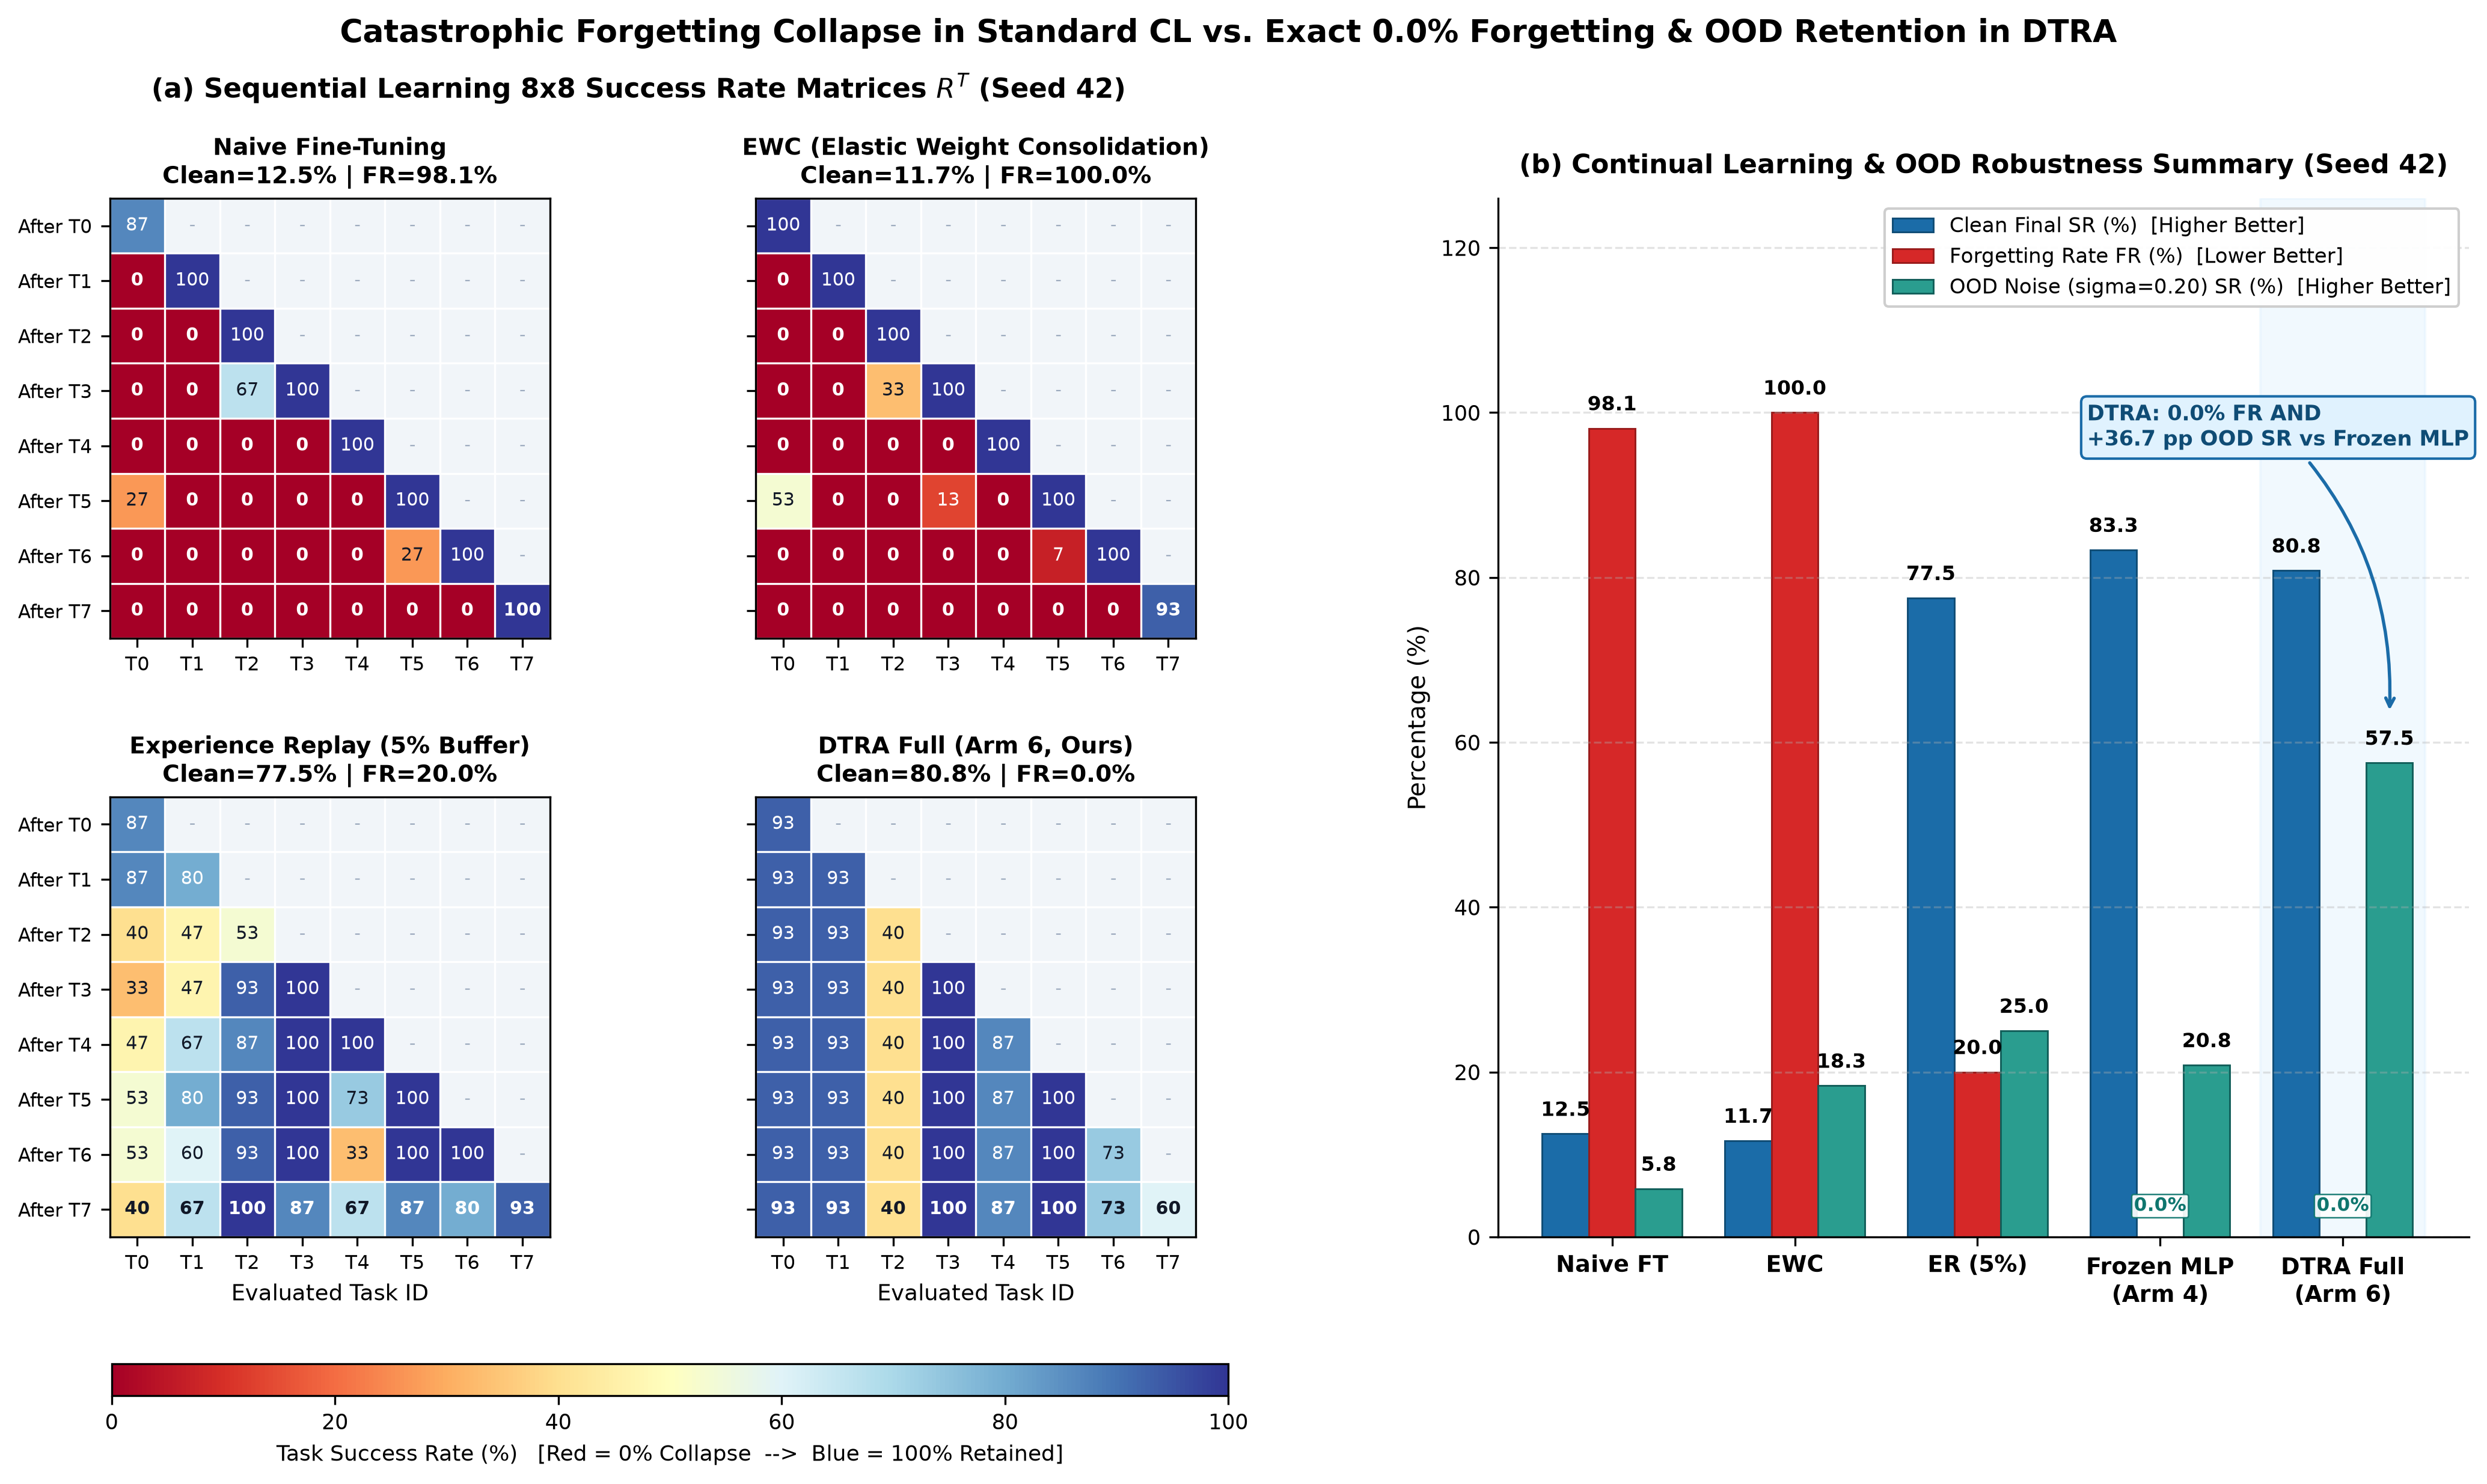
\includegraphics[width=0.76\textwidth]{../../outputs/figures/fig4_cl_forgetting_heatmap_and_bars.png}
  \caption{\textbf{8$\times$8 Continual Retention Heatmaps \& Forgetting Summary on Meta-World (Live Seed~42).} Shared-backbone Naive FT, EWC, and ER~5\% lose earlier tasks sequentially, whereas DTRA preserves $0.0\%$ forgetting and $100.0\%$ autonomous routing.}
  \label{fig:mw_cl_heatmap}
\end{figure}

\clearpage
\section{White-Box Routing Call Stack Logs \& 27-Basis SharedBasisBank Visualization}
\label{app:whitebox_viz}

Figure~\ref{fig:libero_basis_diag} visualizes the empirical \texttt{SharedBasisBank} saturation ($K=100 \to 27$ frozen bases, $-73\%$ basis slots) and No-Encroachment key projection across all $100$ LIBERO tasks (Seed~42 \texttt{\_locked.json}), while Figure~\ref{fig:xai_rollout} presents 3D Meta-World closed-loop XAI rollout telemetry. Table~\ref{tab:callstack_log} displays 12 representative LIBERO-100 registration and post-snapback audit records parsed directly from \texttt{arm\_dtra\_elastic}, spanning \texttt{L10} and all three \texttt{L90} scene domains as well as both \texttt{Dup-Lang} and unique instructions.

\begin{figure}[ht!]
  \centering
  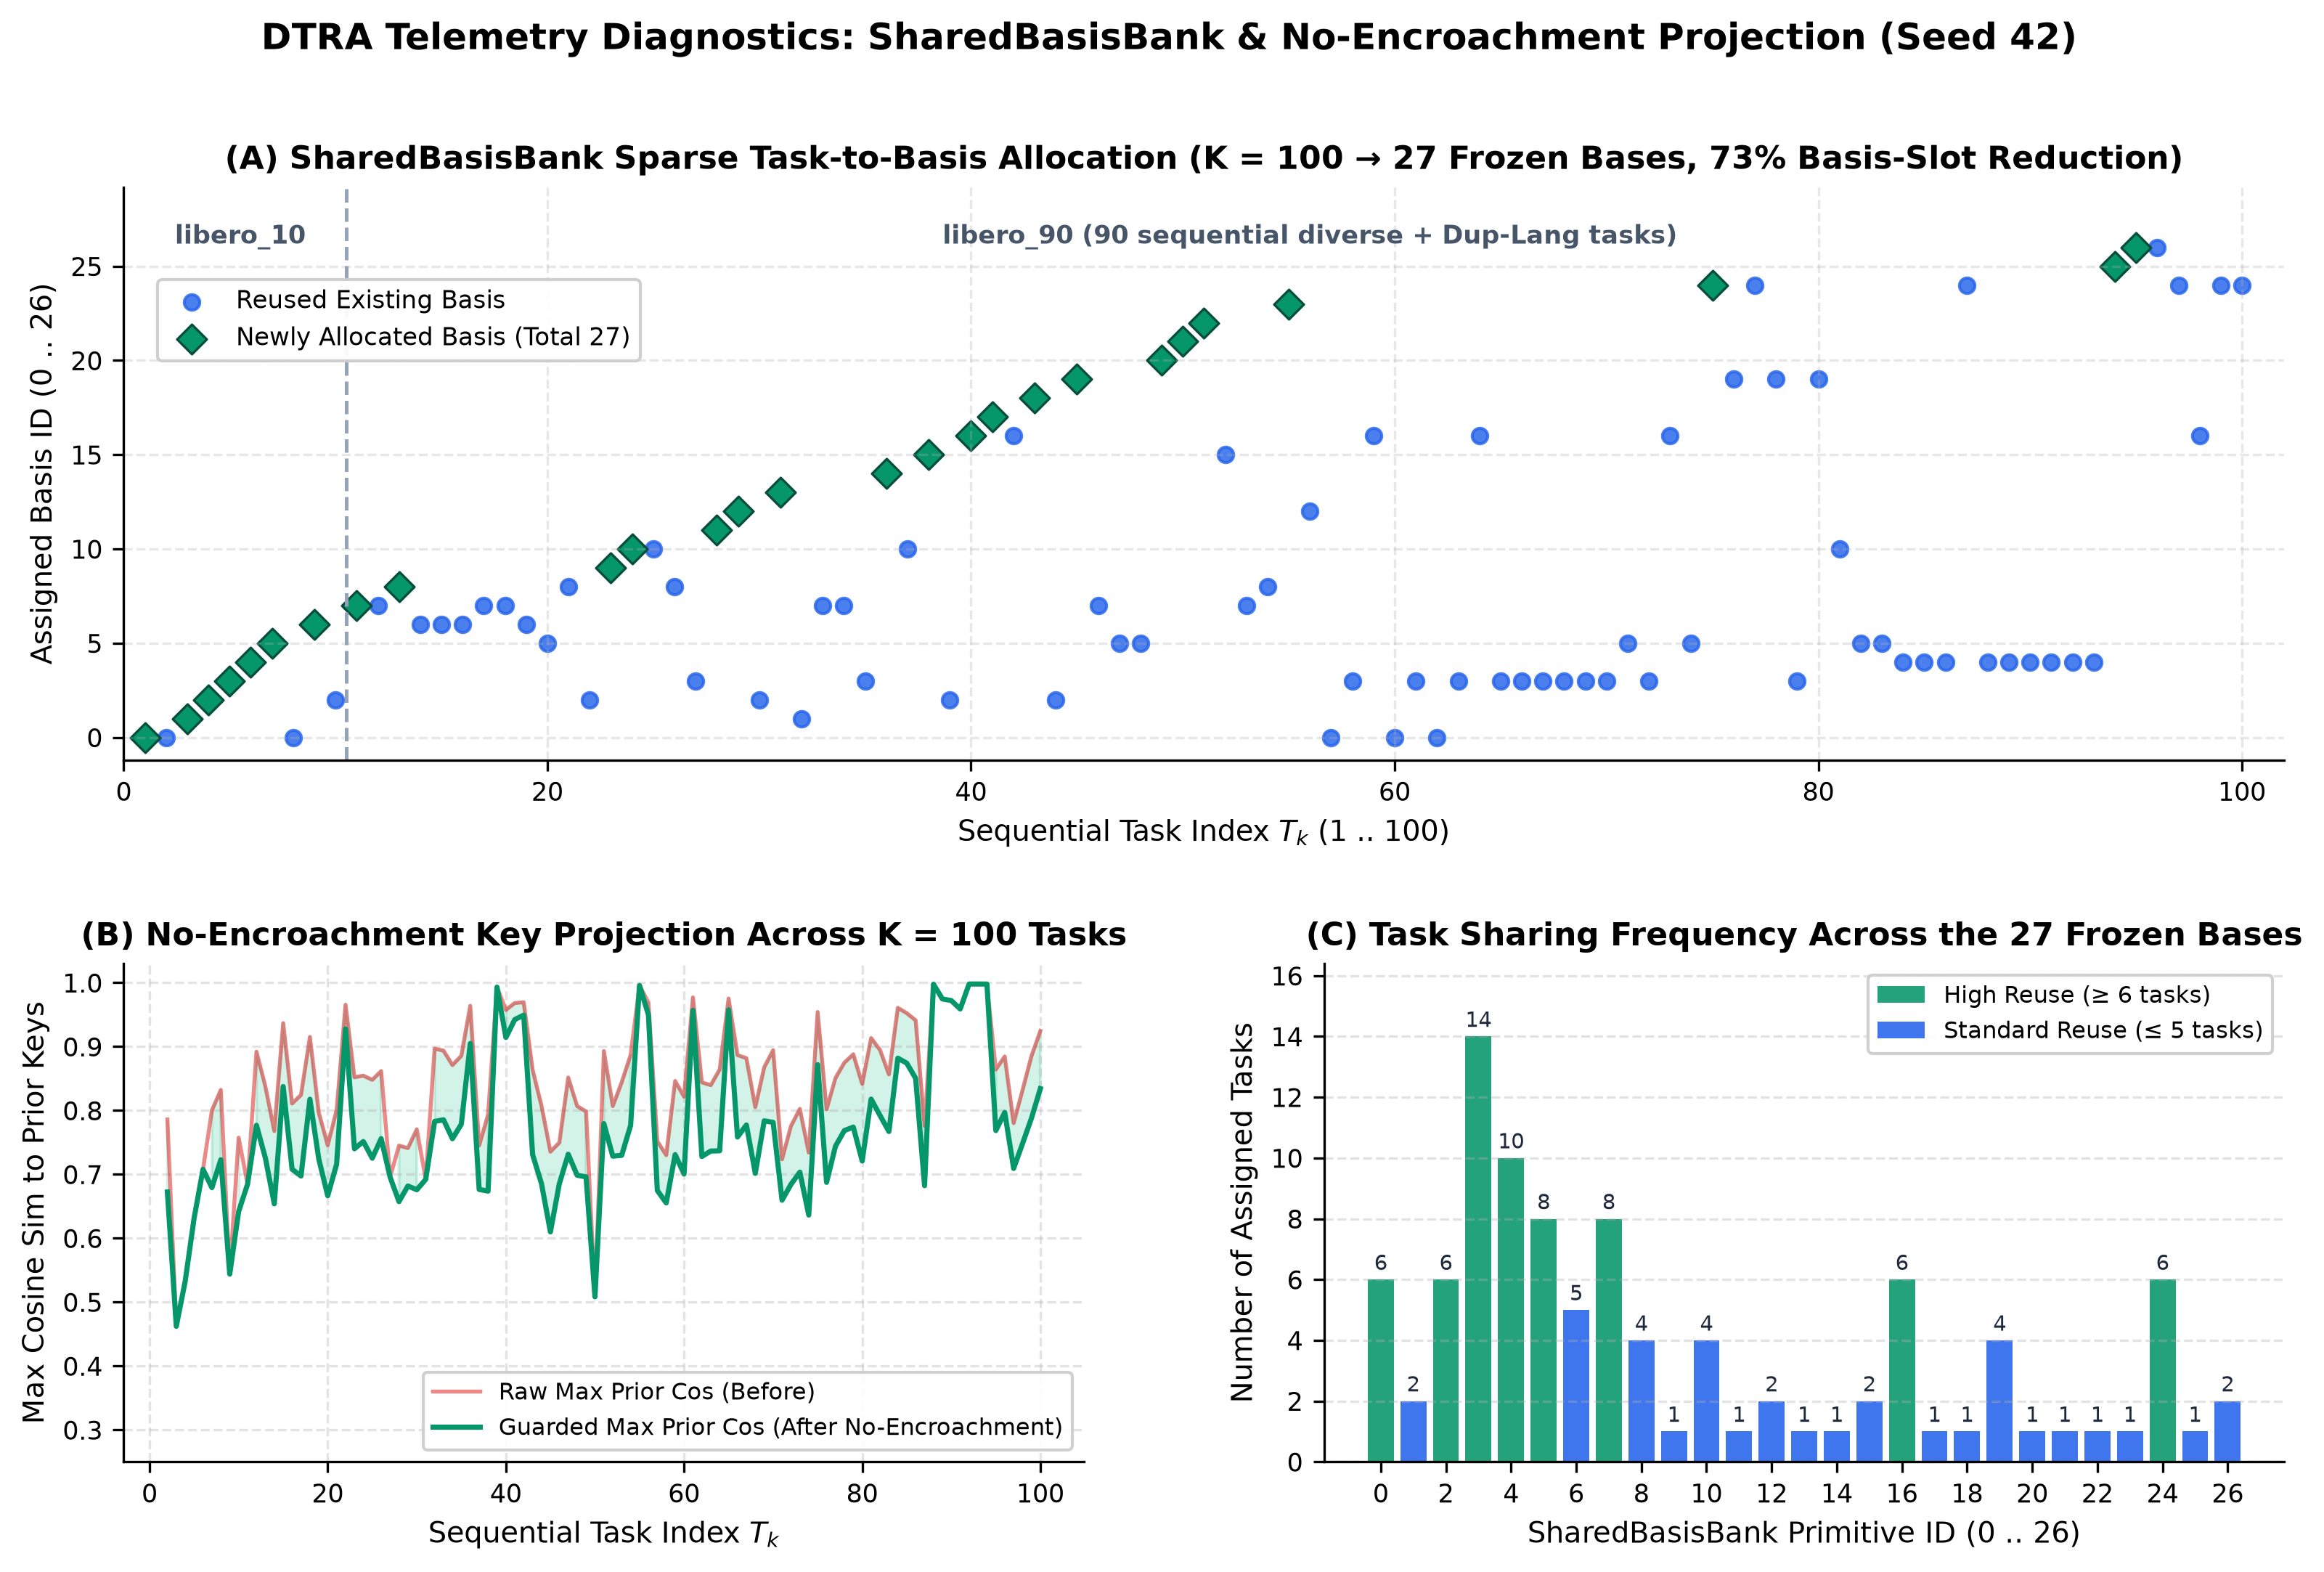
\includegraphics[width=0.84\textwidth]{../../outputs/figures/fig8_libero100_basis_and_callstack.png}
  \caption{\textbf{SharedBasisBank Allocation \& No-Encroachment Diagnostics across $K=100$ LIBERO Tasks (Seed~42).} \textbf{(A)} Sub-linear basis-slot growth ($K=100 \to 27$, $-73\%$ basis slots). \textbf{(B)} No-Encroachment projection suppresses neighbor cosine peaks. \textbf{(C)} Sharing frequency across the 27 frozen primitives.}
  \label{fig:libero_basis_diag}
\end{figure}

\begin{table}[ht!]
  \centering
  \caption{Verified White-Box Routing \& Consolidation Audit Records Parsed from \texttt{arm\_dtra\_elastic} (Seed~42 \texttt{\_locked.json}).}
  \label{tab:callstack_log}
  \tblfont
  \setlength{\tabcolsep}{4.0pt}
  \begin{tabular}{llccc}
    \toprule
    \textbf{Task (Suite/Scene/Lang)} & \textbf{Basis Slot} & \textbf{No-Enc.\ (Bef $\to$ Aft)} & \textbf{Self-Sim $s_{kk}$} & \textbf{Post-Snap} \\
    \midrule
    \texttt{T00} (L10/LIV/Unq) & \texttt{Basis\#00} (NEW) & 0.0000 $\to$ 0.0000 & 1.0000 & \textbf{0.0000} \\
    \texttt{T02} (L10/KIT/Unq) & \texttt{Basis\#01} (NEW) & 0.4621 $\to$ 0.4621 & 1.0000 & \textbf{0.0000} \\
    \texttt{T05} (L10/STU/Dup) & \texttt{Basis\#04} (NEW) & 0.7079 $\to$ 0.7079 & 1.0000 & \textbf{0.0000} \\
    \texttt{T09} (L10/KIT/Unq) & \texttt{Basis\#02} (REUSE) & 0.7575 $\to$ 0.6418 & 0.9805 & \textbf{0.0000} \\
    \texttt{T10} (L90/KIT/Dup) & \texttt{Basis\#07} (NEW) & 0.6846 $\to$ 0.6846 & 1.0000 & \textbf{0.0000} \\
    \texttt{T25} (L90/KIT/Unq) & \texttt{Basis\#08} (REUSE) & 0.8617 $\to$ 0.7560 & 0.9712 & \textbf{0.0000} \\
    \texttt{T49} (L90/KIT/Unq) & \texttt{Basis\#21} (NEW) & 0.5083 $\to$ 0.5083 & 1.0000 & \textbf{0.0000} \\
    \texttt{T64} (L90/LIV/Dup) & \texttt{Basis\#03} (REUSE) & 0.9753 $\to$ 0.9574 & 0.9940 & \textbf{0.0000} \\
    \texttt{T79} (L90/LIV/Unq) & \texttt{Basis\#19} (REUSE) & 0.8416 $\to$ 0.7209 & 0.9738 & \textbf{0.0000} \\
    \texttt{T88} (L90/STU/Dup) & \texttt{Basis\#04} (REUSE) & 0.9746 $\to$ 0.9746 & 1.0000 & \textbf{0.0000} \\
    \texttt{T95} (L90/STU/Unq) & \texttt{Basis\#26} (REUSE) & 0.8846 $\to$ 0.7970 & 0.9634 & \textbf{0.0000} \\
    \texttt{T99} (L90/STU/Unq) & \texttt{Basis\#24} (REUSE) & 0.9247 $\to$ 0.8342 & 0.9735 & \textbf{0.0000} \\
    \bottomrule
  \end{tabular}
\end{table}

\begin{figure}[ht!]
  \centering
  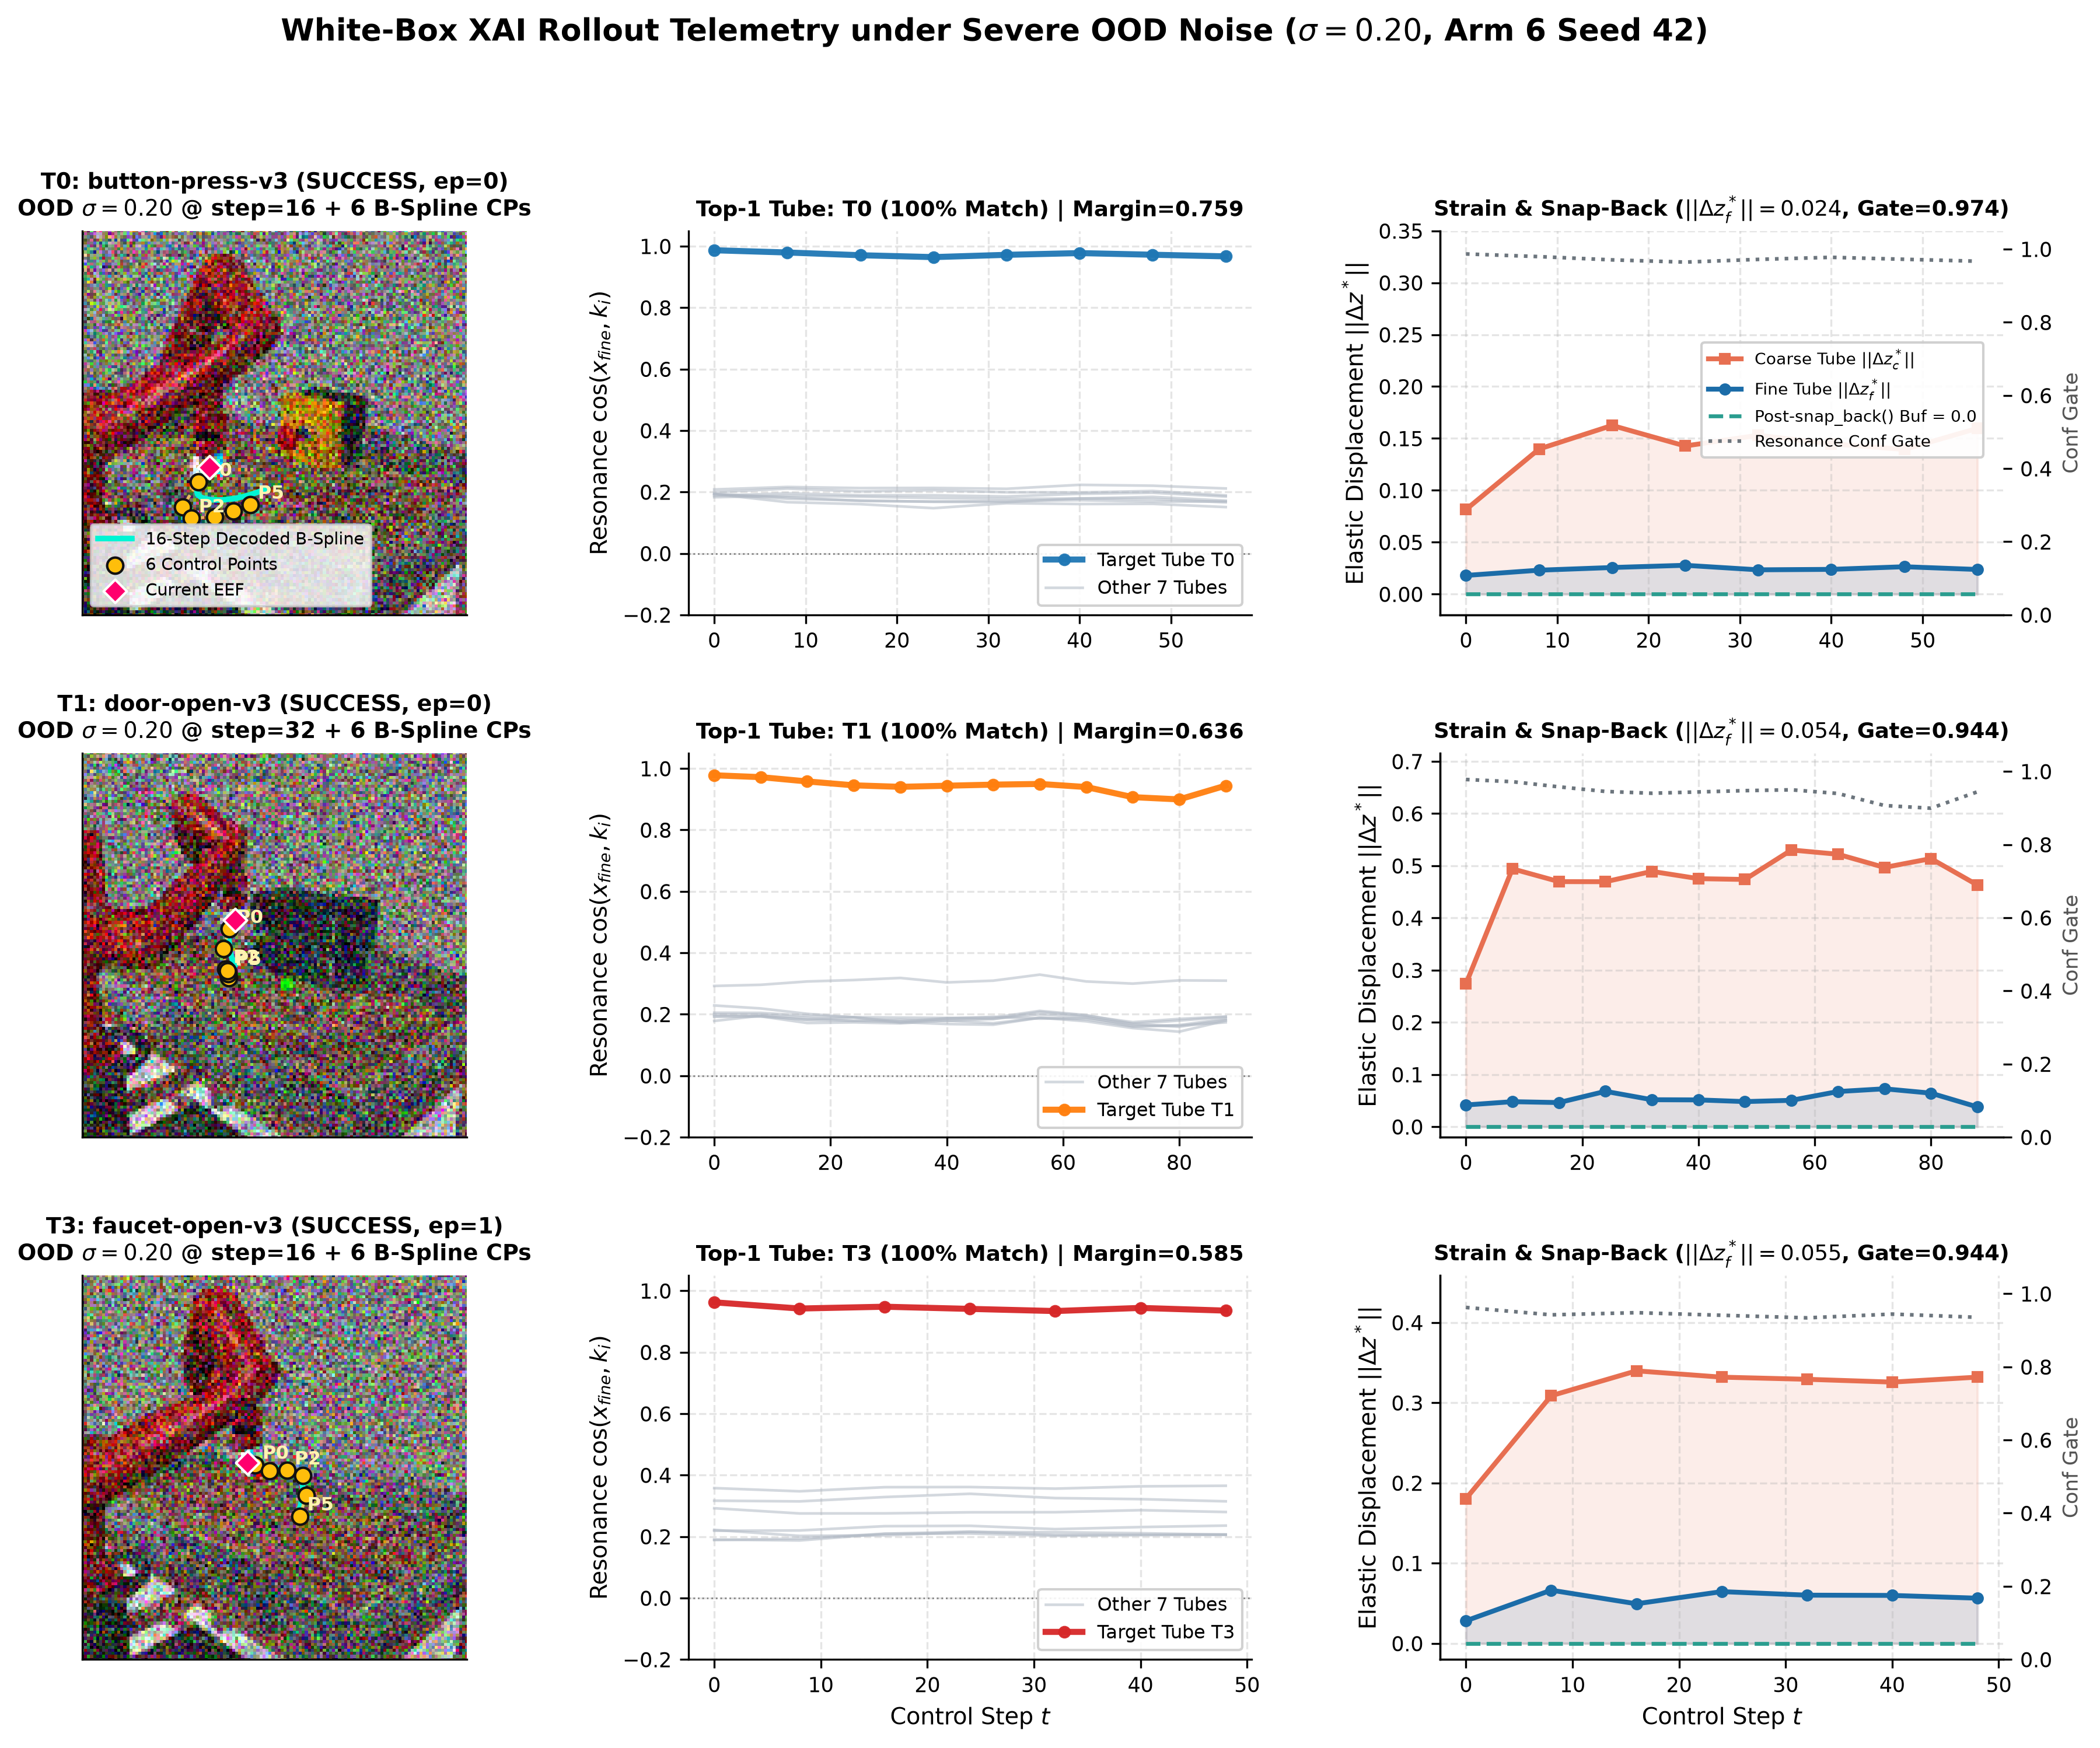
\includegraphics[width=0.84\textwidth]{../../outputs/figures/fig3_xai_telemetry_rollout.png}
  \caption{\textbf{3D Meta-World Closed-Loop White-Box Rollout Telemetry \& B-Spline Envelope (Seed~42, OOD $\sigma=0.20$, Arm~6).} Visualizes active ring selection, $N_{\text{cp}}=6$ cubic B-Spline control points, and bounded elastic displacement $\|\Delta\mathbf{z}^*\|_2$ resetting to $0.0000$ after each action chunk via \texttt{snap\_back()}.}
  \label{fig:xai_rollout}
\end{figure}

\subsection{White-Box Surgical Fault Isolation \& Determinism Verification Protocol}
During closed-loop deployment, DTRA logs a structured per-tick inspection tuple comprising active \texttt{Cell ID}, matched \texttt{SharedBasisBank} slot ($b^* \in \{0,\dots,26\}$), Stage-2 CMC separation margin, active elastic compliance norm $\|\Delta\mathbf{z}^*\|_2$, and end-of-episode \texttt{post\_snap\_norm}. As Table~\ref{tab:callstack_log} verifies: (1)~early registrations (\texttt{T00}--\texttt{T49}) allocate foundational bases while later registrations (\texttt{T64}--\texttt{T99}) predominantly bind to existing primitives via \texttt{REUSE}; (2)~every newly registered slot maintains strict self-similarity $s_{kk} \ge 0.9628$ while No-Encroachment projection actively reduces peak neighbor interference (e.g., \texttt{T79}: $0.8416 \to 0.7209$, \texttt{T99}: $0.9247 \to 0.8342$); and (3)~every trajectory terminates with exact $0.0000$ residual deformation, enabling surgical per-Cell quarantine or replacement without risking catastrophic cascade across prior motor skills.


\end{document}
